\documentclass{article}
\usepackage{graphicx}
\usepackage{geometry}
\usepackage{hyperref}
\usepackage{booktabs}
\usepackage{subcaption}
\usepackage{amsmath}

\geometry{a4paper, margin=0.65in}

\hypersetup{
    colorlinks=true,
    linkcolor=blue,
    filecolor=magenta,
    urlcolor=cyan,
}

\title{MNIST CNN ReLU Clipping Sweep Report:\\No Clip vs.\ Clip 1/2/4 vs.\ Tanh vs.\ Grad-Norm Clip 21}
\author{ByzFL SNN Benchmark}
\date{\today}

\begin{document}

\maketitle

\clearpage
\tableofcontents
\clearpage

\section{Introduction}
This report compares six MNIST CNN configurations:
\begin{enumerate}
    \item \textbf{CNN ReLU (No Clip)}: Standard CNN with ReLU, no activation clipping.
    \item \textbf{CNN ReLU (Clip $=1$)}: ReLU activations clipped elementwise to $[0, 1]$.
    \item \textbf{CNN ReLU (Clip $=2$)}: ReLU activations clipped elementwise to $[0, 2]$.
    \item \textbf{CNN ReLU (Clip $=4$)}: ReLU activations clipped elementwise to $[0, 4]$.
    \item \textbf{CNN Tanh}: CNN with Tanh activation (implicit saturation).
    \item \textbf{CNN ReLU (Grad-Norm Clip $=21$)}: ReLU network with the gradient's overall norm clipped to 21 (not a per-neuron/elementwise clip).
\end{enumerate}

\textbf{Note:} The Grad-Norm Clip $=21$ configuration only has heatmaps available for the best-aggregator (worst-case) sections and the Geometric Median sections.

\clearpage

\section{Best Overall Performance (Worst-Case Across Attacks)}
\begin{figure}[htbp]
    \centering
    \begin{subfigure}[b]{0.32\textwidth}
        \centering
        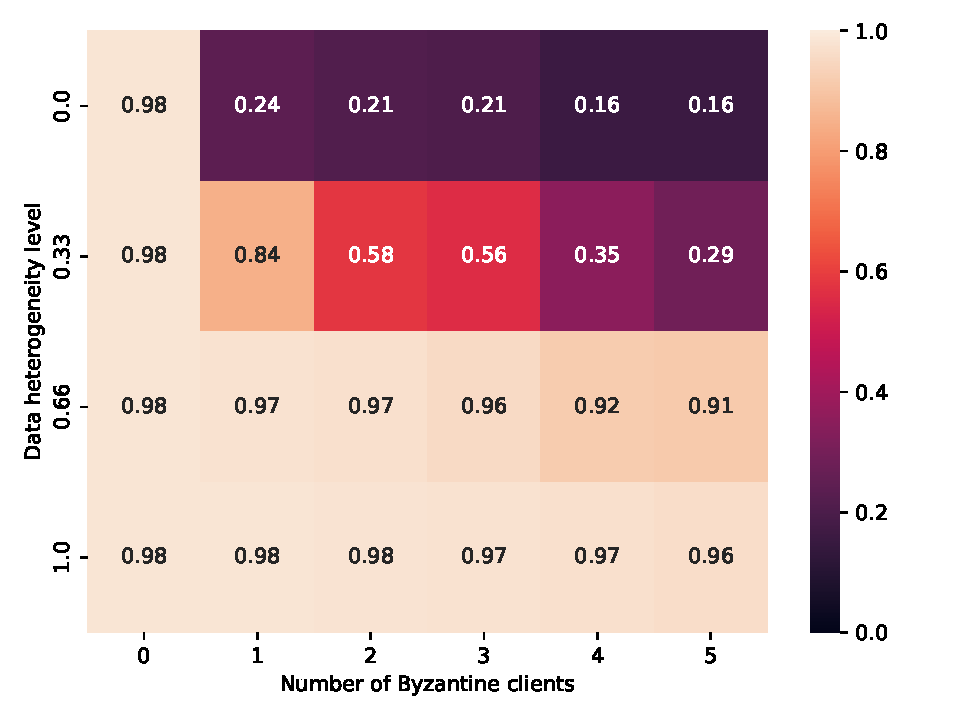
\includegraphics[width=\textwidth]{../plots/mnist_clipping_heatmaps/cnn_mnist/best_test_mnist_cnn_mnist_gamma_similarity_niid_NNM_ARC_nb_honest_clients_10_tolerated_f_equal_real.pdf}
        \caption{CNN ReLU (No Clip)}
        \label{fig:best_overall_noclip}
    \end{subfigure}
    \hfill
    \begin{subfigure}[b]{0.32\textwidth}
        \centering
        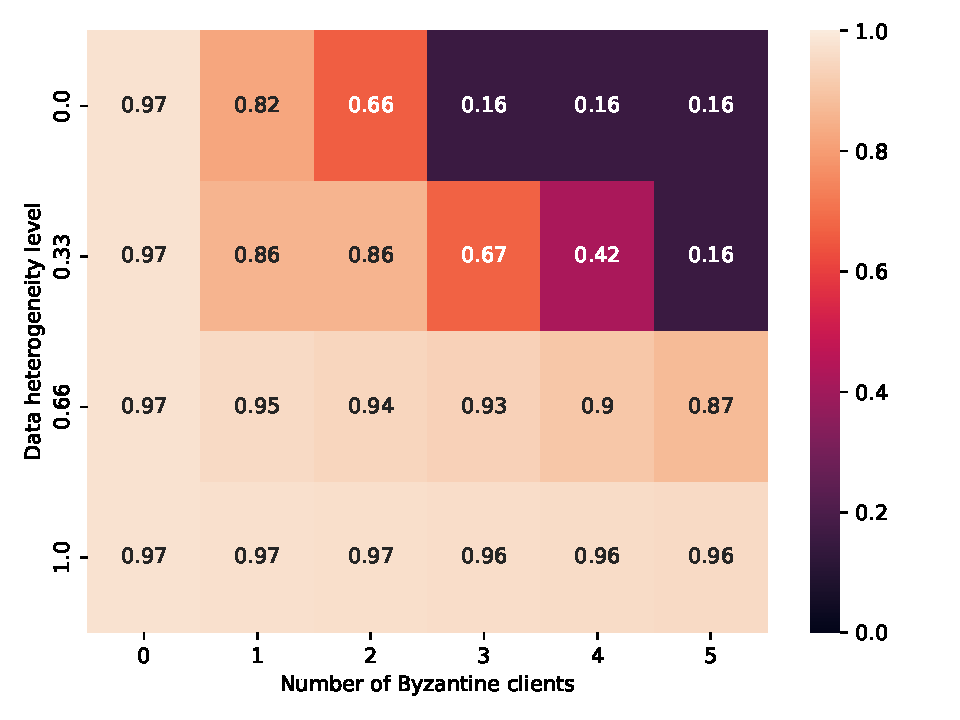
\includegraphics[width=\textwidth]{../plots/mnist_clipping_heatmaps/cnn_mnist_clipping_1/best_test_mnist_cnn_mnist_clipping_1_gamma_similarity_niid_NNM_ARC_nb_honest_clients_10_tolerated_f_equal_real.pdf}
        \caption{CNN ReLU (Clip $=1$)}
        \label{fig:best_overall_clip1}
    \end{subfigure}
    \hfill
    \begin{subfigure}[b]{0.32\textwidth}
        \centering
        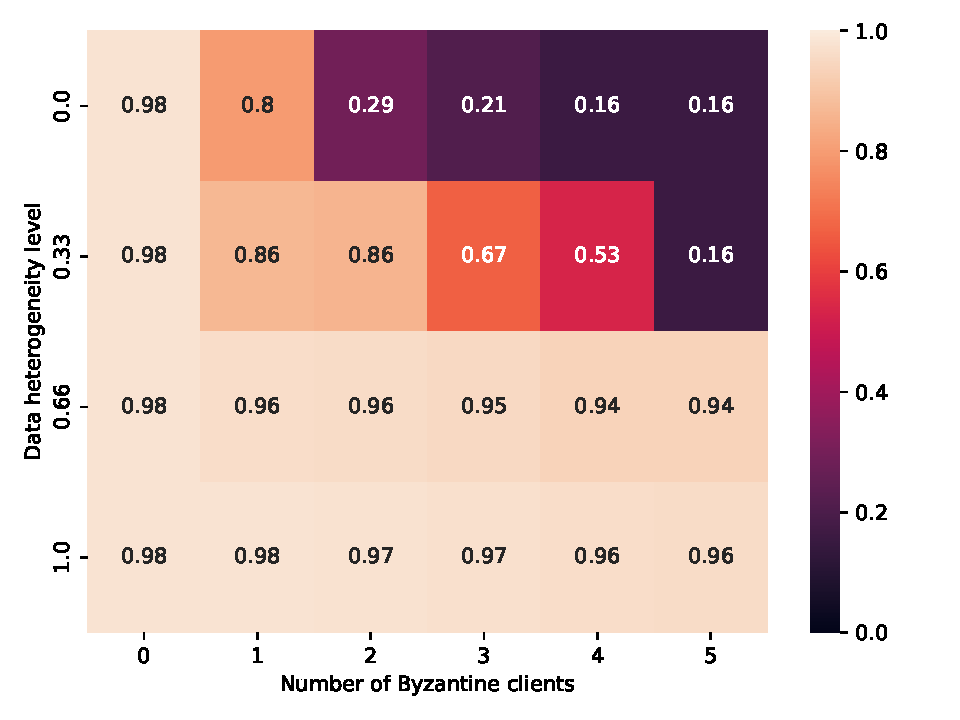
\includegraphics[width=\textwidth]{../plots/mnist_clipping_heatmaps/cnn_mnist_clipping_2/best_test_mnist_cnn_mnist_clipping_2_gamma_similarity_niid_NNM_ARC_nb_honest_clients_10_tolerated_f_equal_real.pdf}
        \caption{CNN ReLU (Clip $=2$)}
        \label{fig:best_overall_clip2}
    \end{subfigure}
    \vspace{0.3cm}
    \begin{subfigure}[b]{0.32\textwidth}
        \centering
        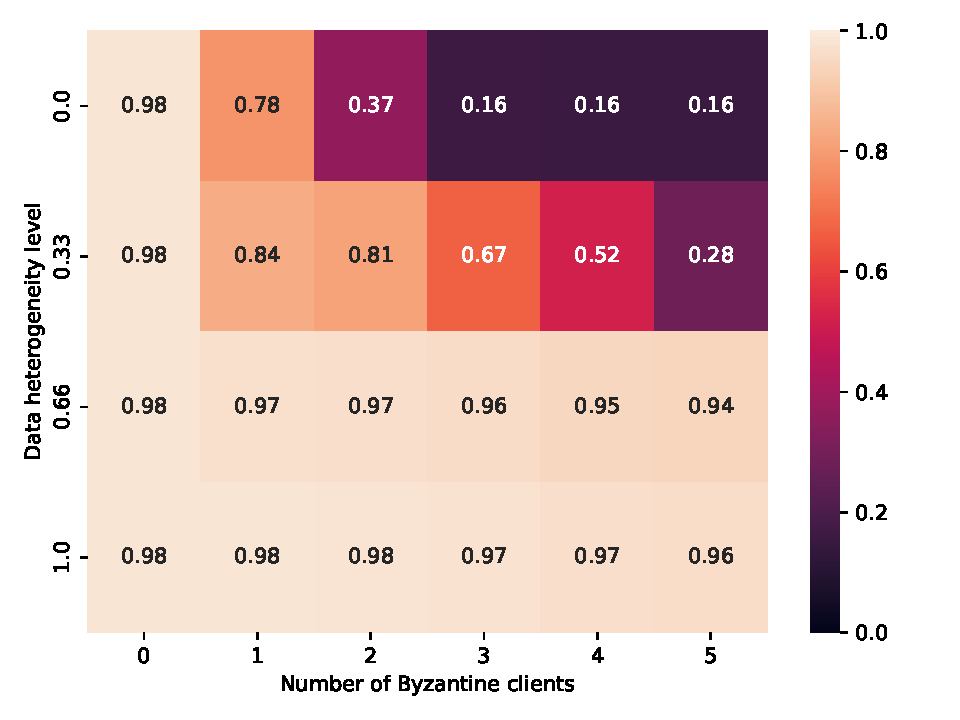
\includegraphics[width=\textwidth]{../plots/mnist_clipping_heatmaps/cnn_mnist_clipping_4/best_test_mnist_cnn_mnist_clipping_4_gamma_similarity_niid_NNM_ARC_nb_honest_clients_10_tolerated_f_equal_real.pdf}
        \caption{CNN ReLU (Clip $=4$)}
        \label{fig:best_overall_clip4}
    \end{subfigure}
    \hfill
    \begin{subfigure}[b]{0.32\textwidth}
        \centering
        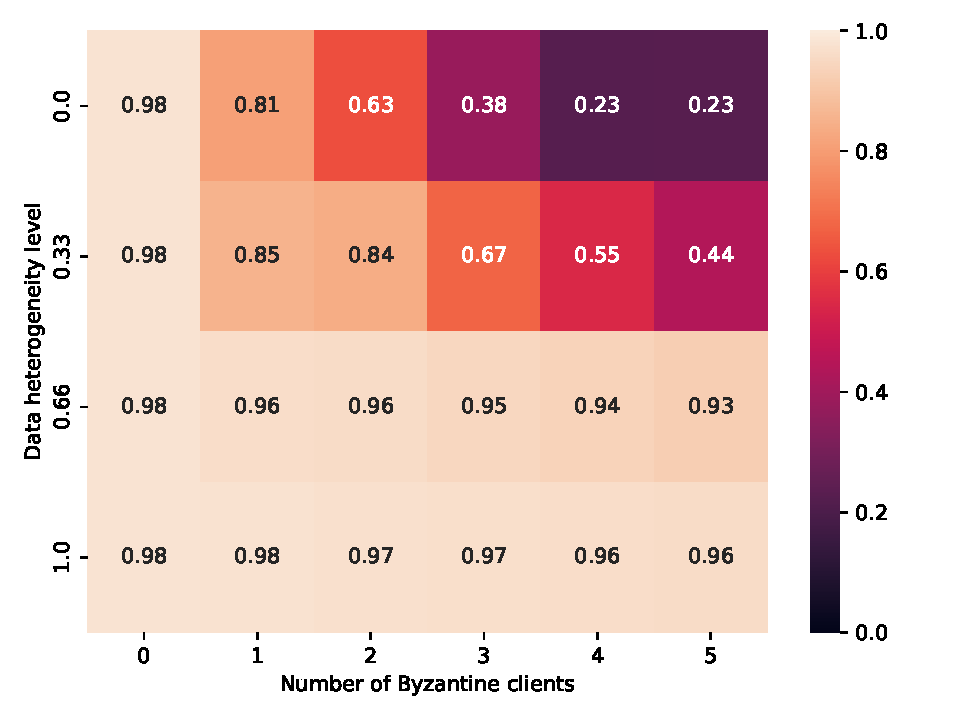
\includegraphics[width=\textwidth]{../plots/cnn_tanh_heatmaps/best_test_mnist_cnn_mnist_tanh_gamma_similarity_niid_NNM_ARC_nb_honest_clients_10_tolerated_f_equal_real.pdf}
        \caption{CNN Tanh}
        \label{fig:best_overall_tanh}
    \end{subfigure}
    \hfill
    \begin{subfigure}[b]{0.32\textwidth}
        \centering
        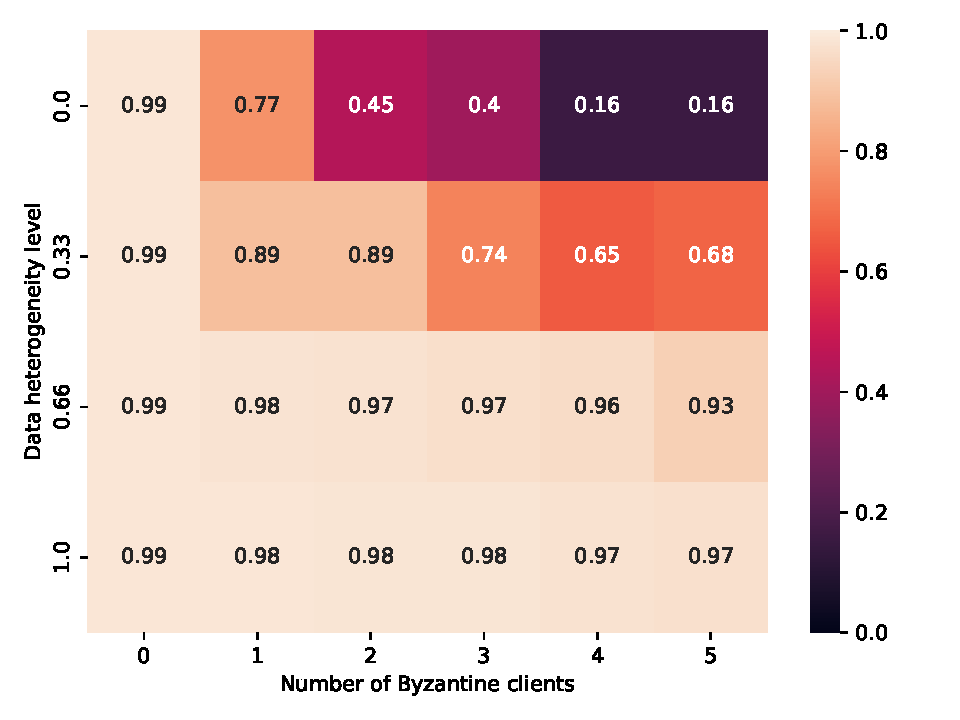
\includegraphics[width=\textwidth]{../plots/cnn_clipped_heatmaps/best_test_mnist_cnn_mnist_gamma_similarity_niid_NNM_ARC_nb_honest_clients_10_tolerated_f_equal_real.pdf}
        \caption{CNN ReLU (Grad-Norm Clip $=21$)}
        \label{fig:best_overall_gradclip21}
    \end{subfigure}
    \caption{Best overall test accuracy (worst-case across attacks).}
    \label{fig:best_overall_grid}
\end{figure}
\clearpage
\section{Best Aggregator under Specific Attacks}

\subsection{Optimal ALIE Attack}
\begin{figure}[htbp]
    \centering
    \begin{subfigure}[b]{0.32\textwidth}
        \centering
        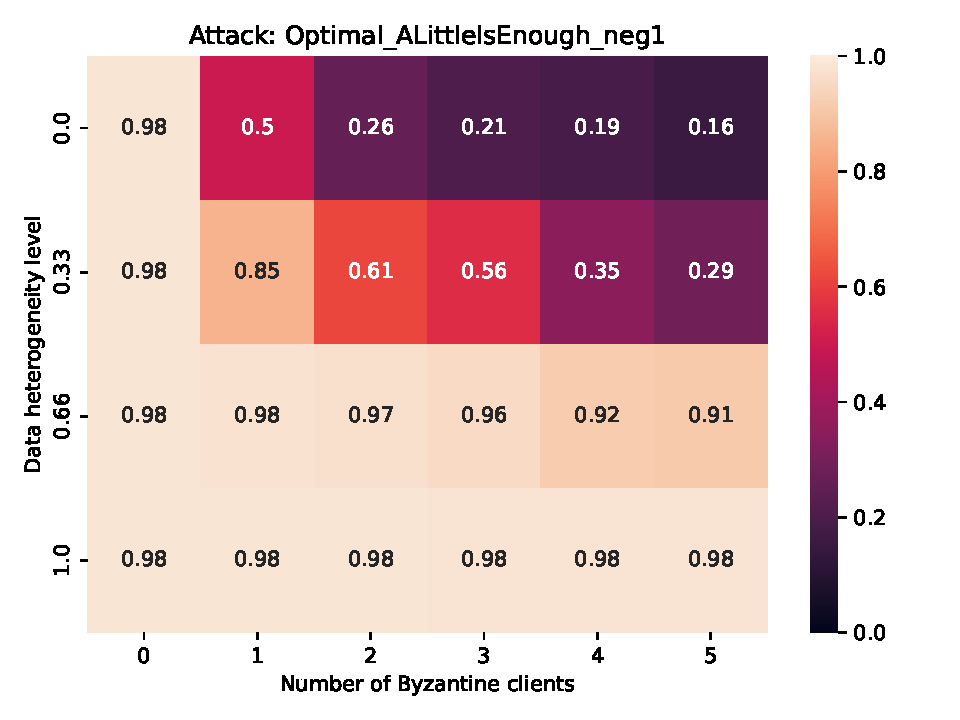
\includegraphics[width=\textwidth]{../plots/mnist_clipping_heatmaps/cnn_mnist/best_test_Optimal_ALittleIsEnough_neg1_mnist_cnn_mnist_gamma_similarity_niid_NNM_ARC_nb_honest_clients_10_tolerated_f_equal_real.pdf}
        \caption{CNN ReLU (No Clip)}
        \label{fig:best_alie_noclip}
    \end{subfigure}
    \hfill
    \begin{subfigure}[b]{0.32\textwidth}
        \centering
        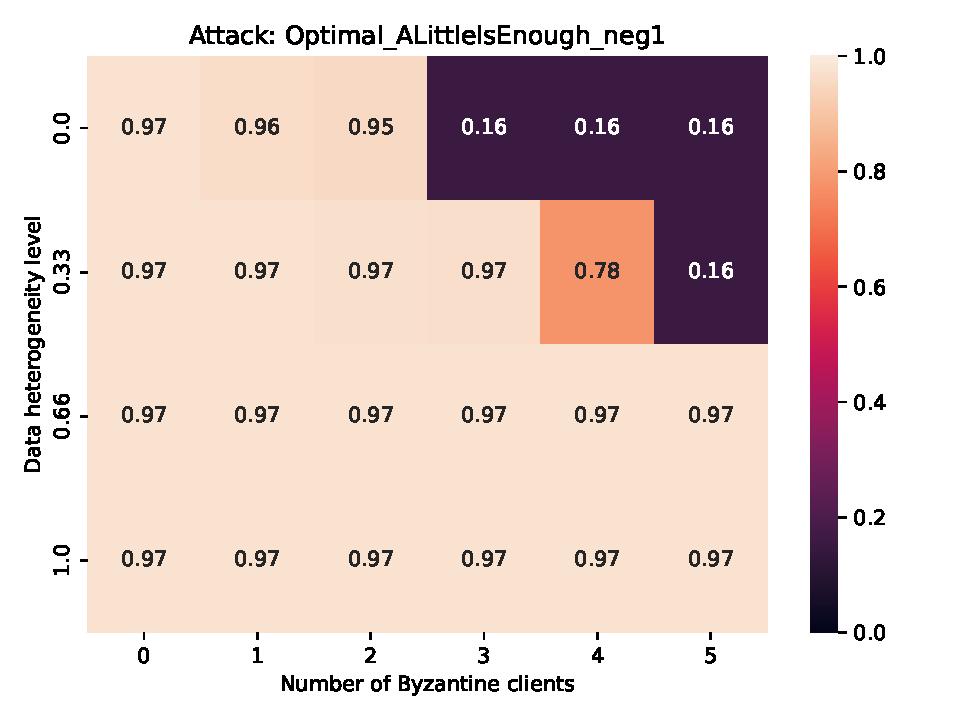
\includegraphics[width=\textwidth]{../plots/mnist_clipping_heatmaps/cnn_mnist_clipping_1/best_test_Optimal_ALittleIsEnough_neg1_mnist_cnn_mnist_clipping_1_gamma_similarity_niid_NNM_ARC_nb_honest_clients_10_tolerated_f_equal_real.pdf}
        \caption{CNN ReLU (Clip $=1$)}
        \label{fig:best_alie_clip1}
    \end{subfigure}
    \hfill
    \begin{subfigure}[b]{0.32\textwidth}
        \centering
        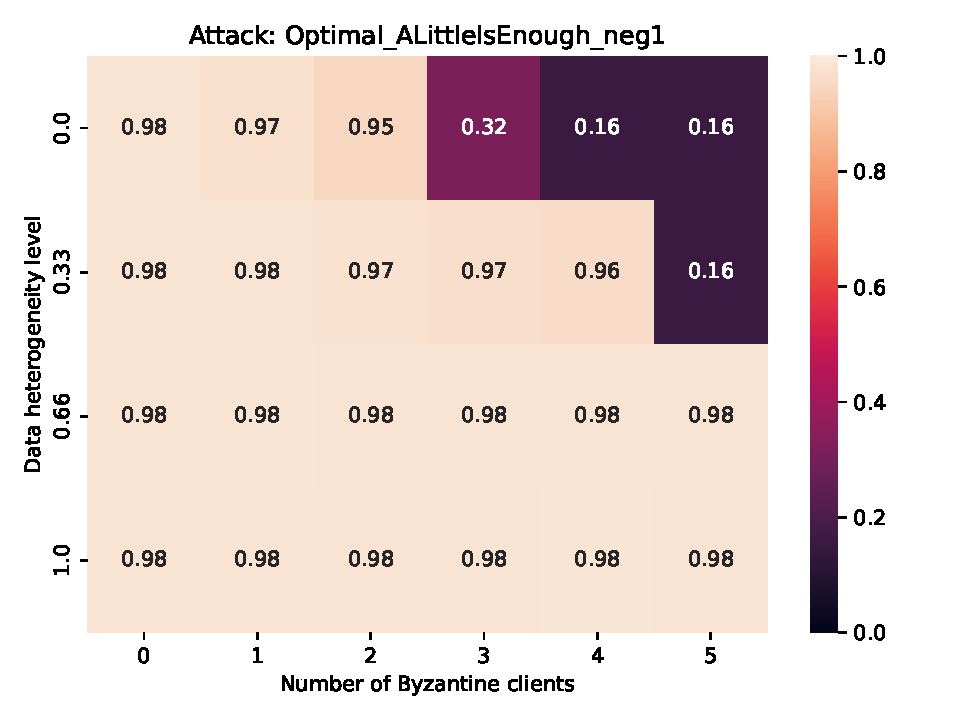
\includegraphics[width=\textwidth]{../plots/mnist_clipping_heatmaps/cnn_mnist_clipping_2/best_test_Optimal_ALittleIsEnough_neg1_mnist_cnn_mnist_clipping_2_gamma_similarity_niid_NNM_ARC_nb_honest_clients_10_tolerated_f_equal_real.pdf}
        \caption{CNN ReLU (Clip $=2$)}
        \label{fig:best_alie_clip2}
    \end{subfigure}
    \vspace{0.3cm}
    \begin{subfigure}[b]{0.32\textwidth}
        \centering
        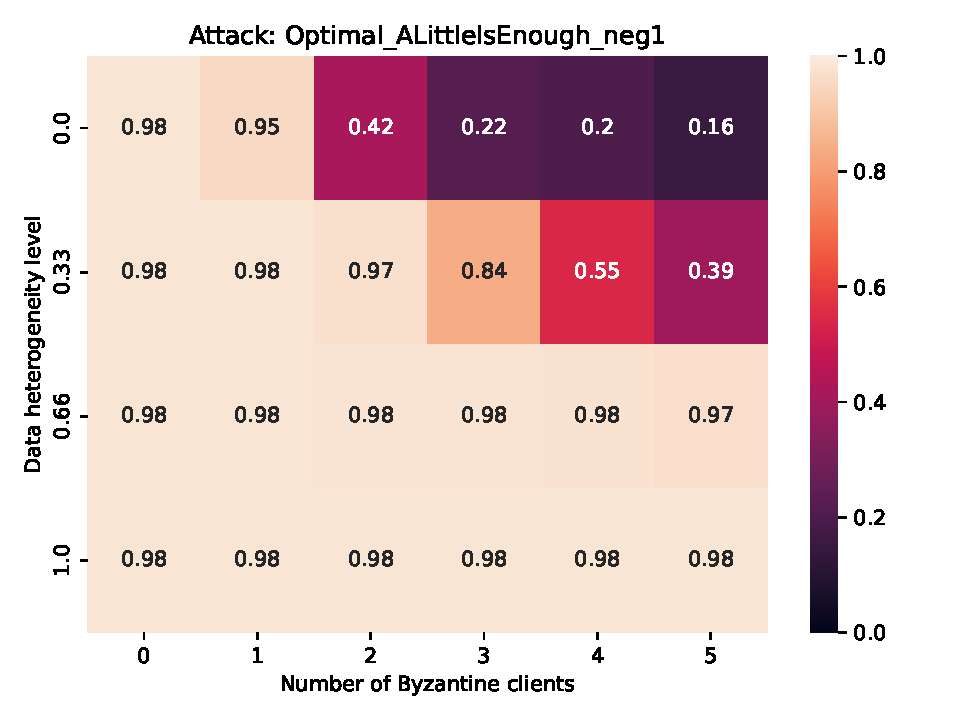
\includegraphics[width=\textwidth]{../plots/mnist_clipping_heatmaps/cnn_mnist_clipping_4/best_test_Optimal_ALittleIsEnough_neg1_mnist_cnn_mnist_clipping_4_gamma_similarity_niid_NNM_ARC_nb_honest_clients_10_tolerated_f_equal_real.pdf}
        \caption{CNN ReLU (Clip $=4$)}
        \label{fig:best_alie_clip4}
    \end{subfigure}
    \hfill
    \begin{subfigure}[b]{0.32\textwidth}
        \centering
        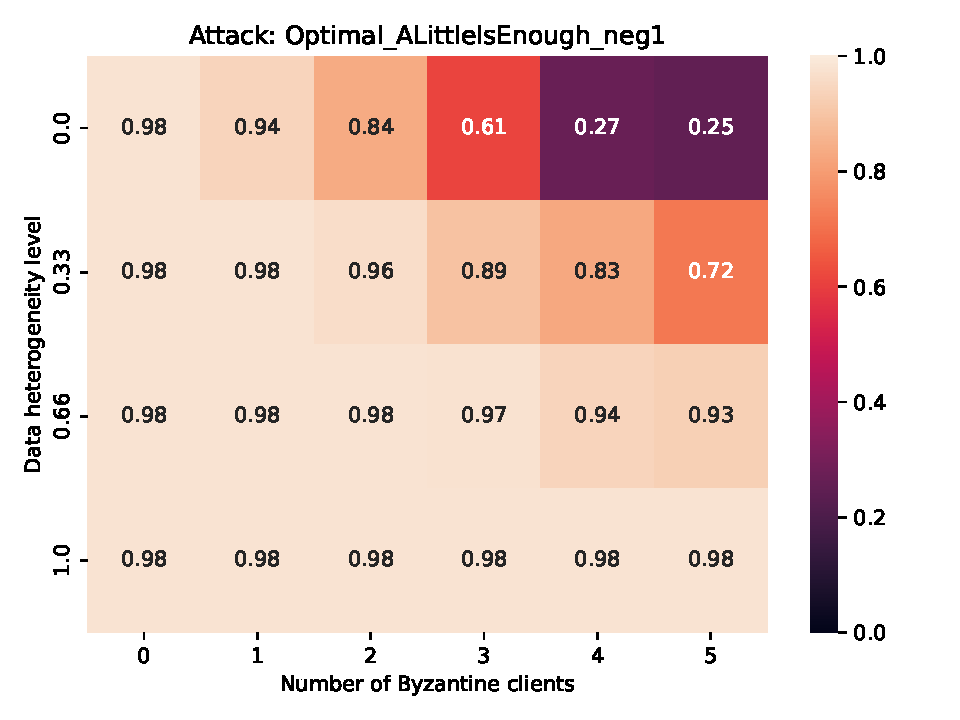
\includegraphics[width=\textwidth]{../plots/cnn_tanh_heatmaps/best_test_Optimal_ALittleIsEnough_neg1_mnist_cnn_mnist_tanh_gamma_similarity_niid_NNM_ARC_nb_honest_clients_10_tolerated_f_equal_real.pdf}
        \caption{CNN Tanh}
        \label{fig:best_alie_tanh}
    \end{subfigure}
    \hfill
    \begin{subfigure}[b]{0.32\textwidth}
        \centering
        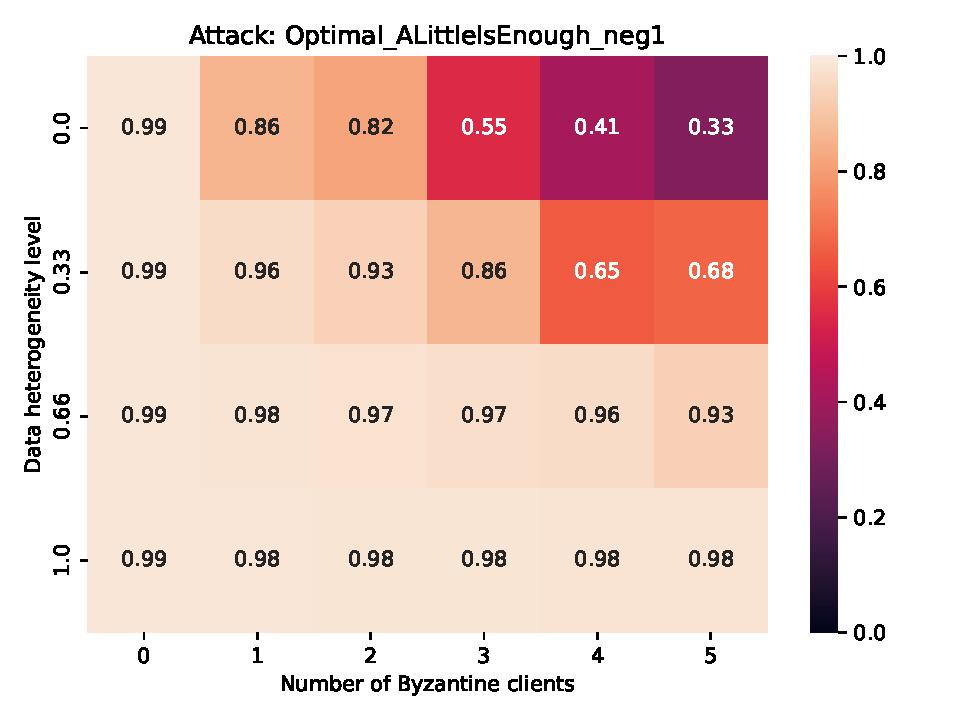
\includegraphics[width=\textwidth]{../plots/cnn_clipped_heatmaps/best_test_Optimal_ALittleIsEnough_neg1_mnist_cnn_mnist_gamma_similarity_niid_NNM_ARC_nb_honest_clients_10_tolerated_f_equal_real.pdf}
        \caption{CNN ReLU (Grad-Norm Clip $=21$)}
        \label{fig:best_alie_gradclip21}
    \end{subfigure}
    \caption{Best test accuracy under ALIE.}
    \label{fig:best_alie_grid}
\end{figure}
\clearpage
\subsection{Sign Flipping Attack}
\begin{figure}[htbp]
    \centering
    \begin{subfigure}[b]{0.32\textwidth}
        \centering
        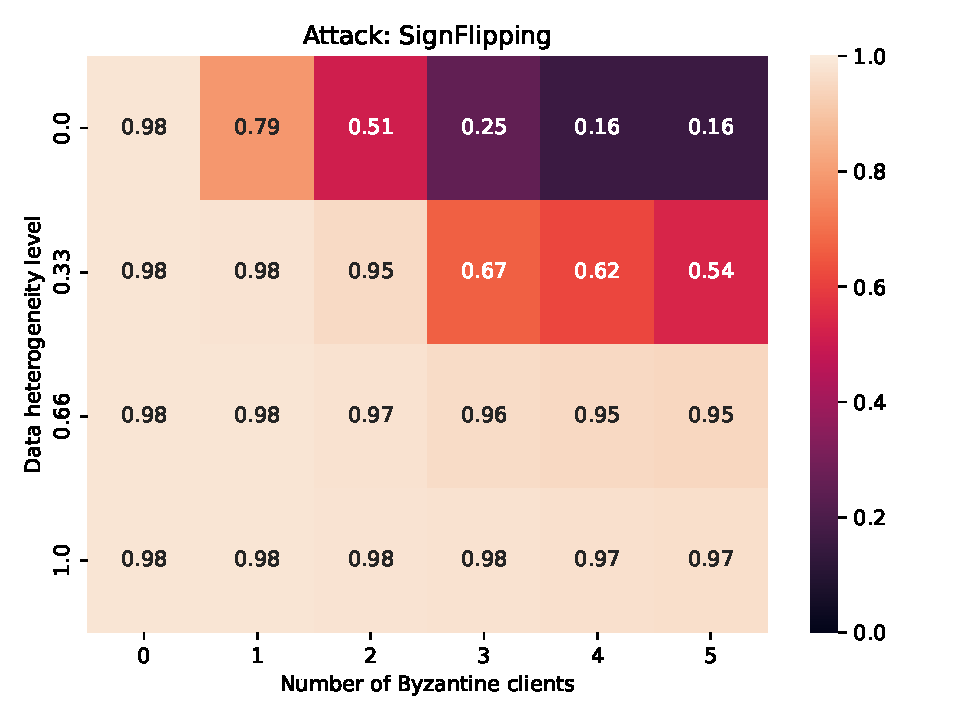
\includegraphics[width=\textwidth]{../plots/mnist_clipping_heatmaps/cnn_mnist/best_test_SignFlipping_mnist_cnn_mnist_gamma_similarity_niid_NNM_ARC_nb_honest_clients_10_tolerated_f_equal_real.pdf}
        \caption{CNN ReLU (No Clip)}
        \label{fig:best_sf_noclip}
    \end{subfigure}
    \hfill
    \begin{subfigure}[b]{0.32\textwidth}
        \centering
        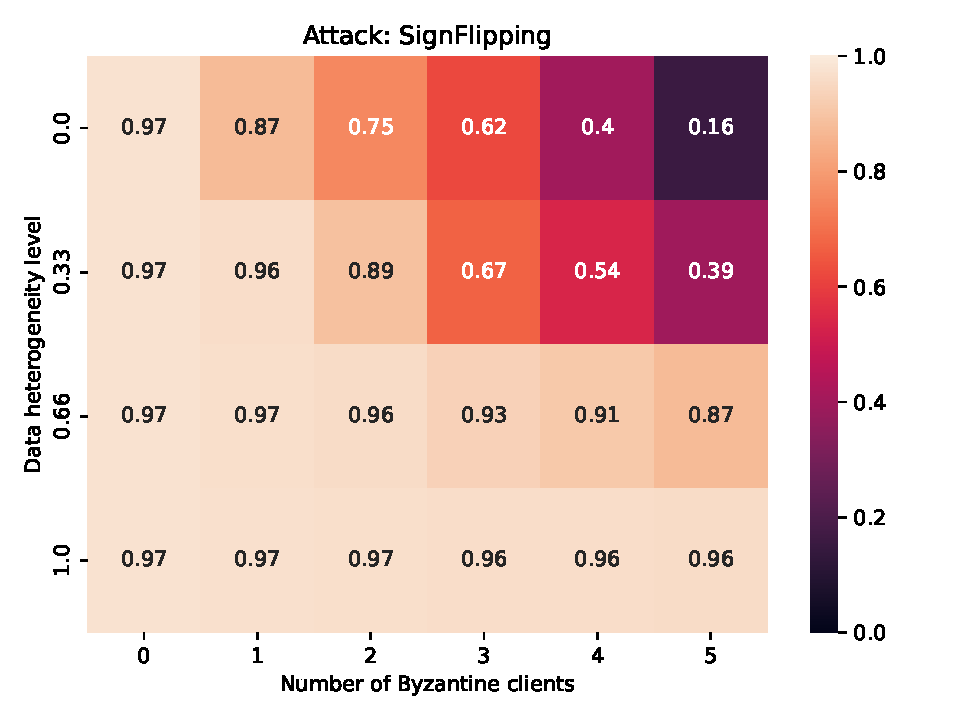
\includegraphics[width=\textwidth]{../plots/mnist_clipping_heatmaps/cnn_mnist_clipping_1/best_test_SignFlipping_mnist_cnn_mnist_clipping_1_gamma_similarity_niid_NNM_ARC_nb_honest_clients_10_tolerated_f_equal_real.pdf}
        \caption{CNN ReLU (Clip $=1$)}
        \label{fig:best_sf_clip1}
    \end{subfigure}
    \hfill
    \begin{subfigure}[b]{0.32\textwidth}
        \centering
        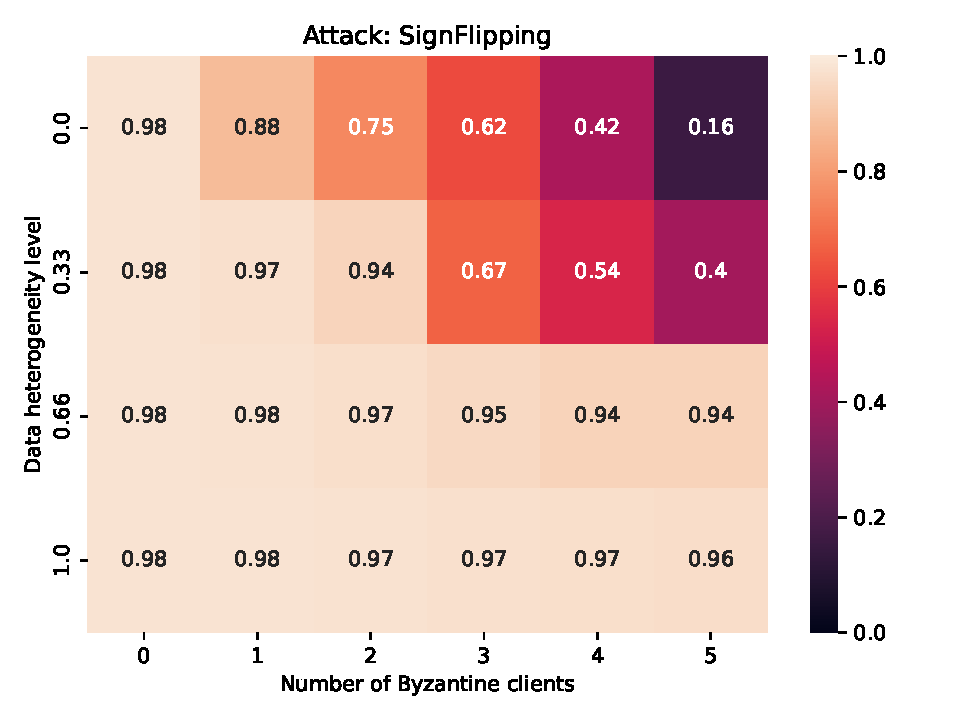
\includegraphics[width=\textwidth]{../plots/mnist_clipping_heatmaps/cnn_mnist_clipping_2/best_test_SignFlipping_mnist_cnn_mnist_clipping_2_gamma_similarity_niid_NNM_ARC_nb_honest_clients_10_tolerated_f_equal_real.pdf}
        \caption{CNN ReLU (Clip $=2$)}
        \label{fig:best_sf_clip2}
    \end{subfigure}
    \vspace{0.3cm}
    \begin{subfigure}[b]{0.32\textwidth}
        \centering
        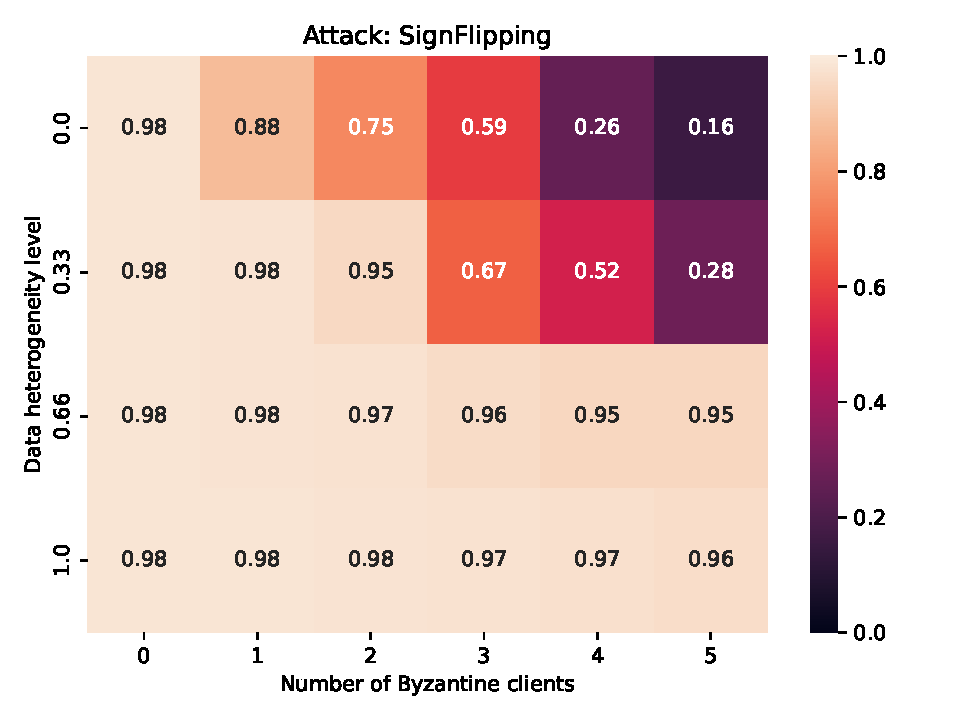
\includegraphics[width=\textwidth]{../plots/mnist_clipping_heatmaps/cnn_mnist_clipping_4/best_test_SignFlipping_mnist_cnn_mnist_clipping_4_gamma_similarity_niid_NNM_ARC_nb_honest_clients_10_tolerated_f_equal_real.pdf}
        \caption{CNN ReLU (Clip $=4$)}
        \label{fig:best_sf_clip4}
    \end{subfigure}
    \hfill
    \begin{subfigure}[b]{0.32\textwidth}
        \centering
        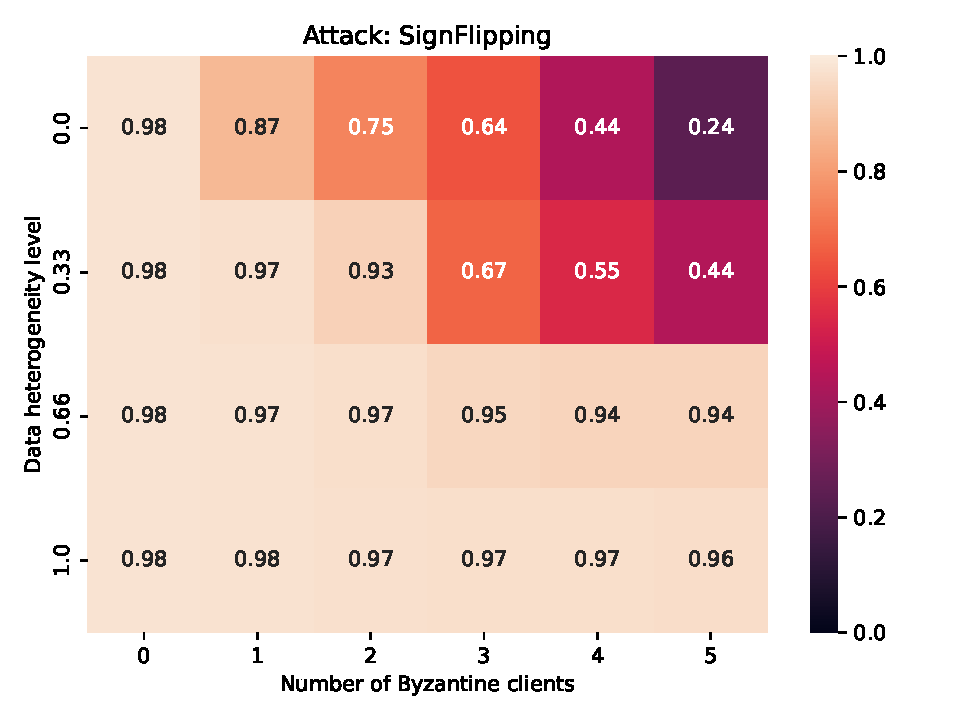
\includegraphics[width=\textwidth]{../plots/cnn_tanh_heatmaps/best_test_SignFlipping_mnist_cnn_mnist_tanh_gamma_similarity_niid_NNM_ARC_nb_honest_clients_10_tolerated_f_equal_real.pdf}
        \caption{CNN Tanh}
        \label{fig:best_sf_tanh}
    \end{subfigure}
    \hfill
    \begin{subfigure}[b]{0.32\textwidth}
        \centering
        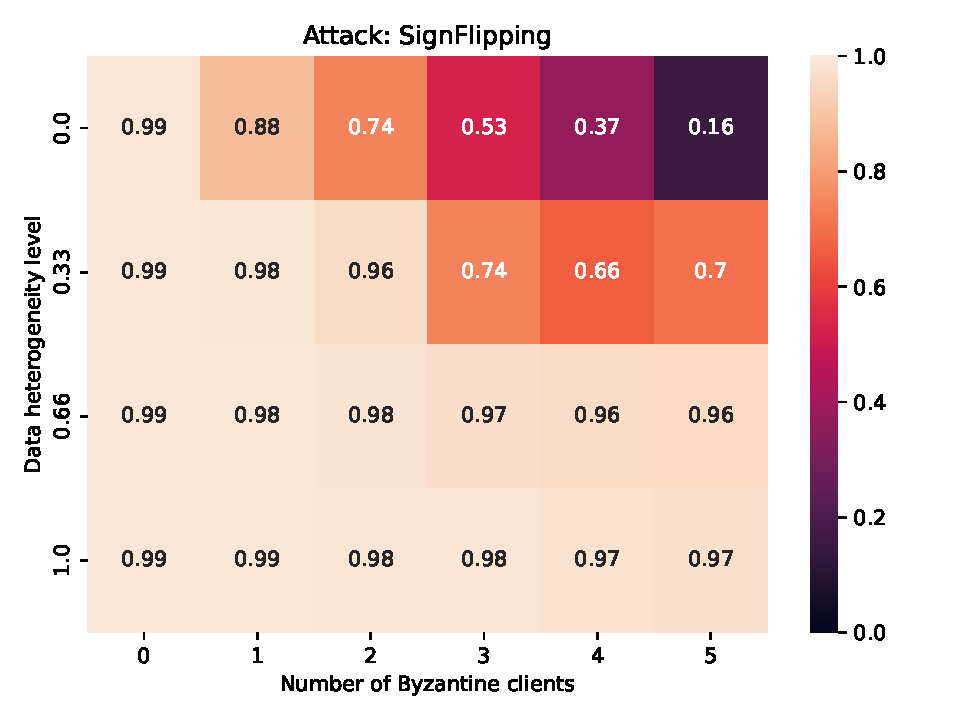
\includegraphics[width=\textwidth]{../plots/cnn_clipped_heatmaps/best_test_SignFlipping_mnist_cnn_mnist_gamma_similarity_niid_NNM_ARC_nb_honest_clients_10_tolerated_f_equal_real.pdf}
        \caption{CNN ReLU (Grad-Norm Clip $=21$)}
        \label{fig:best_sf_gradclip21}
    \end{subfigure}
    \caption{Best test accuracy under SF.}
    \label{fig:best_sf_grid}
\end{figure}
\clearpage
\subsection{Optimal IPM Attack}
\begin{figure}[htbp]
    \centering
    \begin{subfigure}[b]{0.32\textwidth}
        \centering
        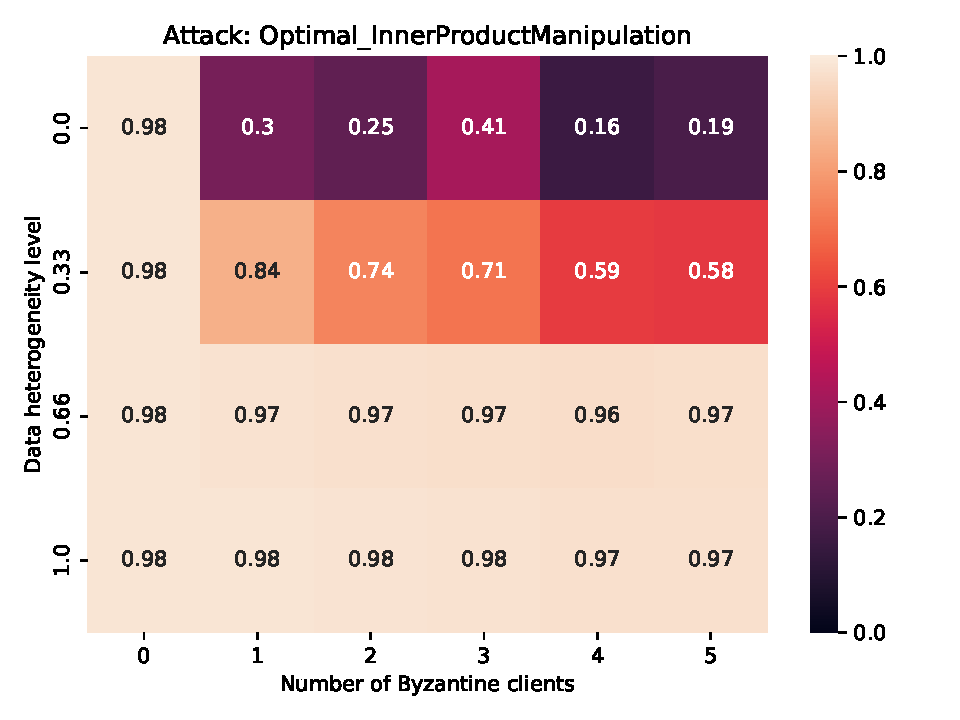
\includegraphics[width=\textwidth]{../plots/mnist_clipping_heatmaps/cnn_mnist/best_test_Optimal_InnerProductManipulation_mnist_cnn_mnist_gamma_similarity_niid_NNM_ARC_nb_honest_clients_10_tolerated_f_equal_real.pdf}
        \caption{CNN ReLU (No Clip)}
        \label{fig:best_ipm_noclip}
    \end{subfigure}
    \hfill
    \begin{subfigure}[b]{0.32\textwidth}
        \centering
        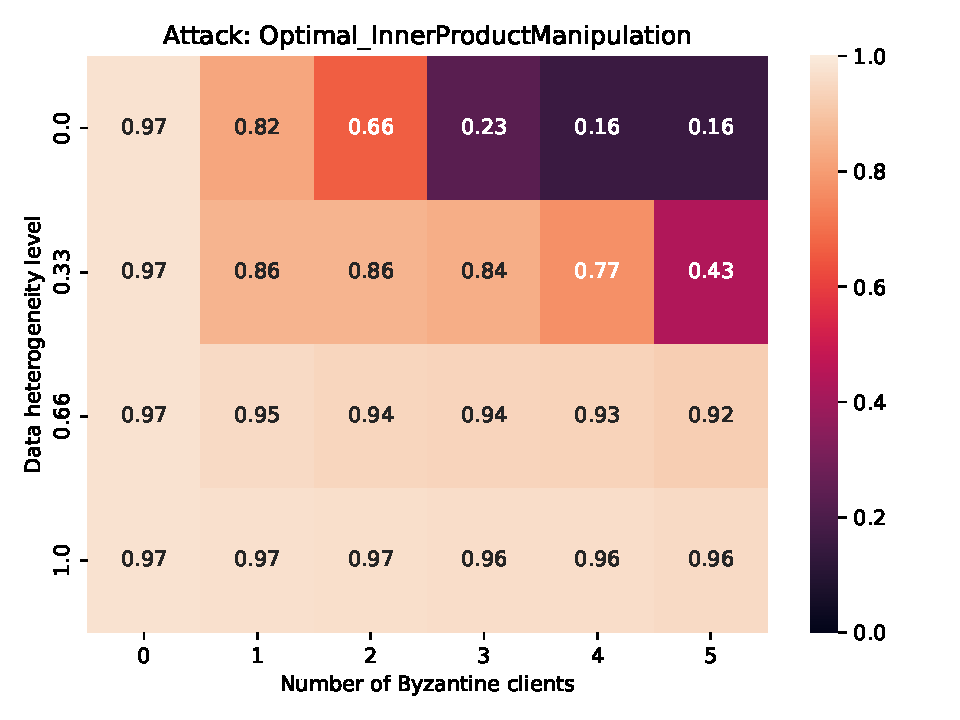
\includegraphics[width=\textwidth]{../plots/mnist_clipping_heatmaps/cnn_mnist_clipping_1/best_test_Optimal_InnerProductManipulation_mnist_cnn_mnist_clipping_1_gamma_similarity_niid_NNM_ARC_nb_honest_clients_10_tolerated_f_equal_real.pdf}
        \caption{CNN ReLU (Clip $=1$)}
        \label{fig:best_ipm_clip1}
    \end{subfigure}
    \hfill
    \begin{subfigure}[b]{0.32\textwidth}
        \centering
        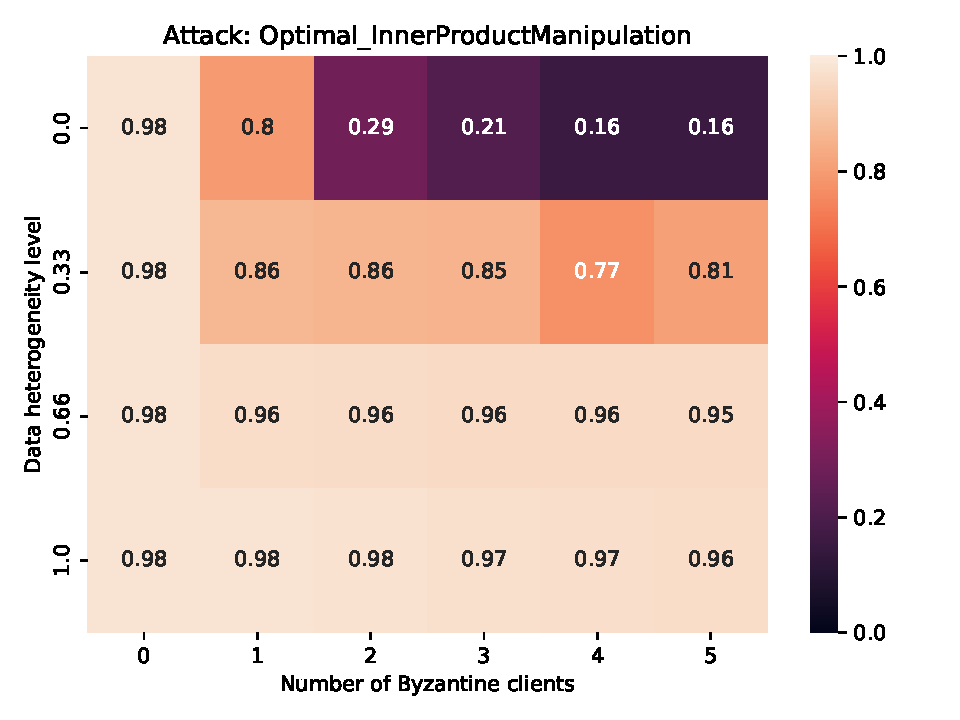
\includegraphics[width=\textwidth]{../plots/mnist_clipping_heatmaps/cnn_mnist_clipping_2/best_test_Optimal_InnerProductManipulation_mnist_cnn_mnist_clipping_2_gamma_similarity_niid_NNM_ARC_nb_honest_clients_10_tolerated_f_equal_real.pdf}
        \caption{CNN ReLU (Clip $=2$)}
        \label{fig:best_ipm_clip2}
    \end{subfigure}
    \vspace{0.3cm}
    \begin{subfigure}[b]{0.32\textwidth}
        \centering
        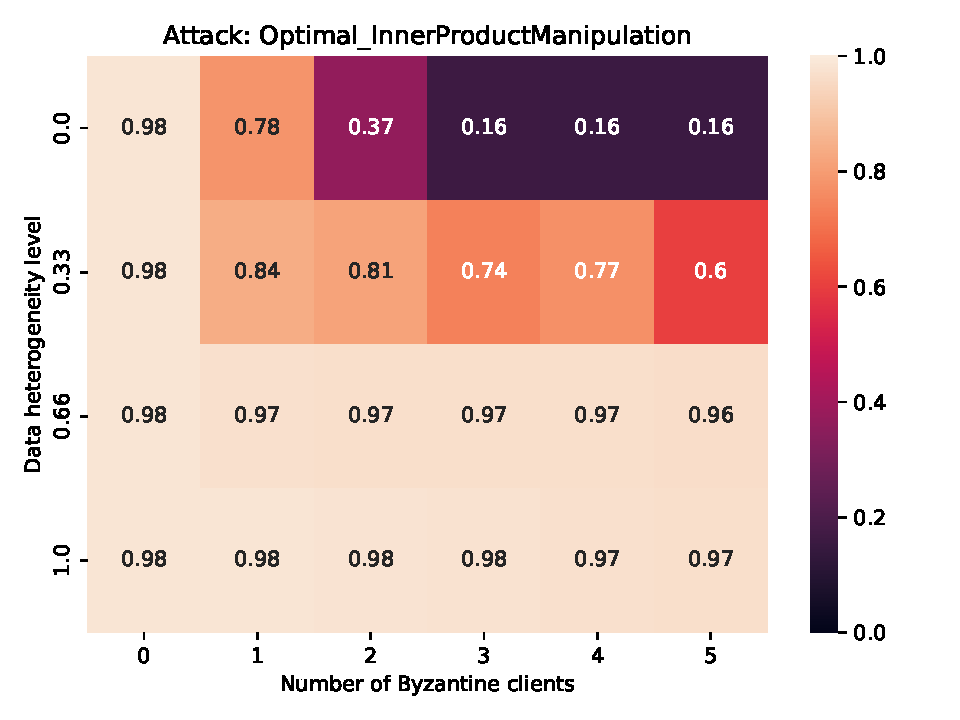
\includegraphics[width=\textwidth]{../plots/mnist_clipping_heatmaps/cnn_mnist_clipping_4/best_test_Optimal_InnerProductManipulation_mnist_cnn_mnist_clipping_4_gamma_similarity_niid_NNM_ARC_nb_honest_clients_10_tolerated_f_equal_real.pdf}
        \caption{CNN ReLU (Clip $=4$)}
        \label{fig:best_ipm_clip4}
    \end{subfigure}
    \hfill
    \begin{subfigure}[b]{0.32\textwidth}
        \centering
        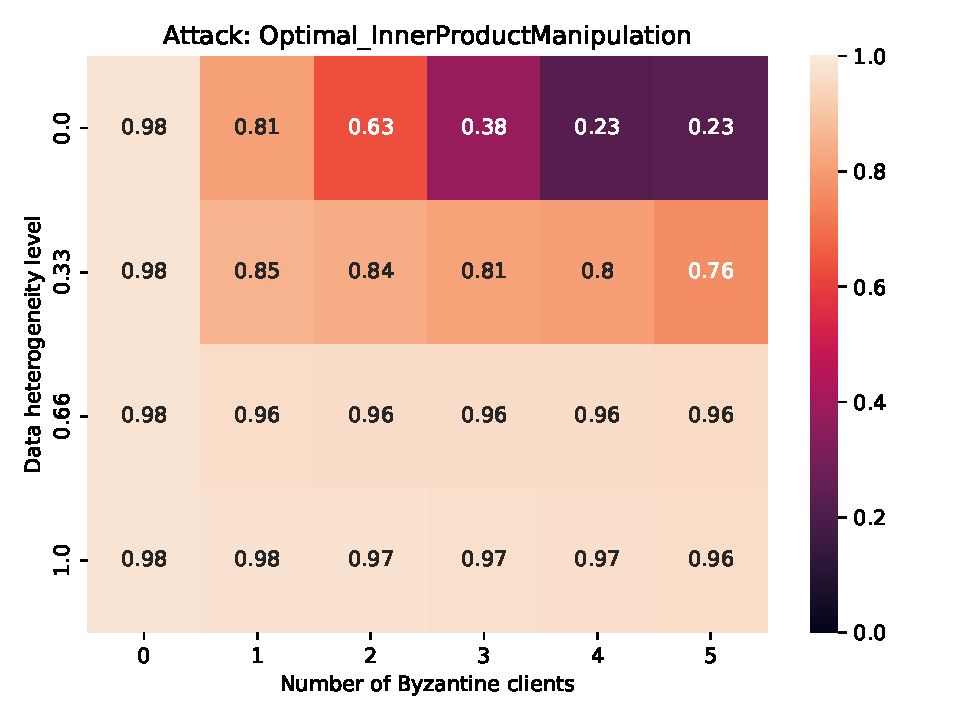
\includegraphics[width=\textwidth]{../plots/cnn_tanh_heatmaps/best_test_Optimal_InnerProductManipulation_mnist_cnn_mnist_tanh_gamma_similarity_niid_NNM_ARC_nb_honest_clients_10_tolerated_f_equal_real.pdf}
        \caption{CNN Tanh}
        \label{fig:best_ipm_tanh}
    \end{subfigure}
    \hfill
    \begin{subfigure}[b]{0.32\textwidth}
        \centering
        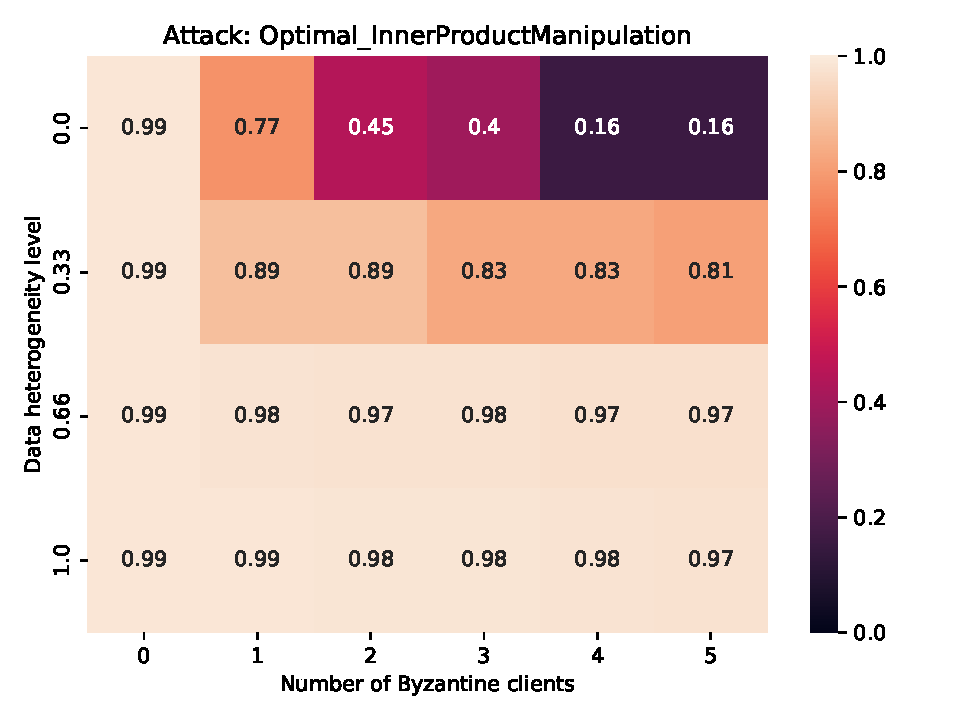
\includegraphics[width=\textwidth]{../plots/cnn_clipped_heatmaps/best_test_Optimal_InnerProductManipulation_mnist_cnn_mnist_gamma_similarity_niid_NNM_ARC_nb_honest_clients_10_tolerated_f_equal_real.pdf}
        \caption{CNN ReLU (Grad-Norm Clip $=21$)}
        \label{fig:best_ipm_gradclip21}
    \end{subfigure}
    \caption{Best test accuracy under IPM.}
    \label{fig:best_ipm_grid}
\end{figure}
\clearpage
\subsection{Centered Clipping (CC)}
\subsubsection{CC under Worst-Case across all Attacks}
\begin{figure}[htbp]
    \centering
    \begin{subfigure}[b]{0.24\textwidth}
        \centering
        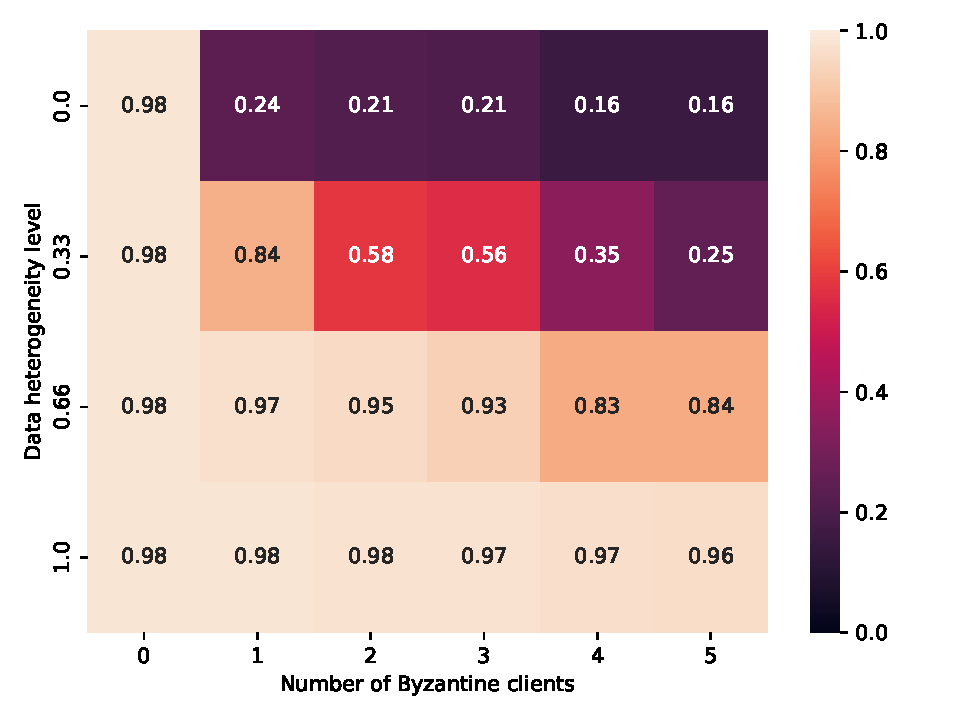
\includegraphics[width=\textwidth]{../plots/mnist_clipping_heatmaps/cnn_mnist/test_mnist_cnn_mnist_gamma_similarity_niid_NNM_ARC_CenteredClipping_nb_honest_clients_10_tolerated_f_equal_real.pdf}
        \caption{CNN ReLU (No Clip)}
        \label{fig:cc_worst_case_noclip}
    \end{subfigure}
    \hfill
    \begin{subfigure}[b]{0.24\textwidth}
        \centering
        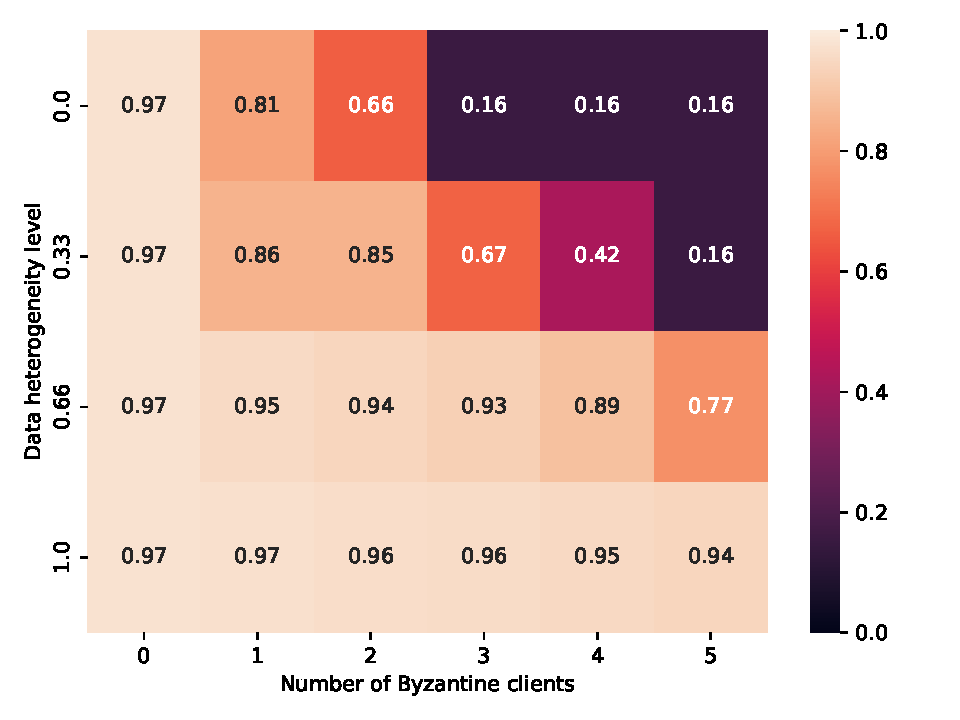
\includegraphics[width=\textwidth]{../plots/mnist_clipping_heatmaps/cnn_mnist_clipping_1/test_mnist_cnn_mnist_clipping_1_gamma_similarity_niid_NNM_ARC_CenteredClipping_nb_honest_clients_10_tolerated_f_equal_real.pdf}
        \caption{CNN ReLU (Clip $=1$)}
        \label{fig:cc_worst_case_clip1}
    \end{subfigure}
    \hfill
    \begin{subfigure}[b]{0.24\textwidth}
        \centering
        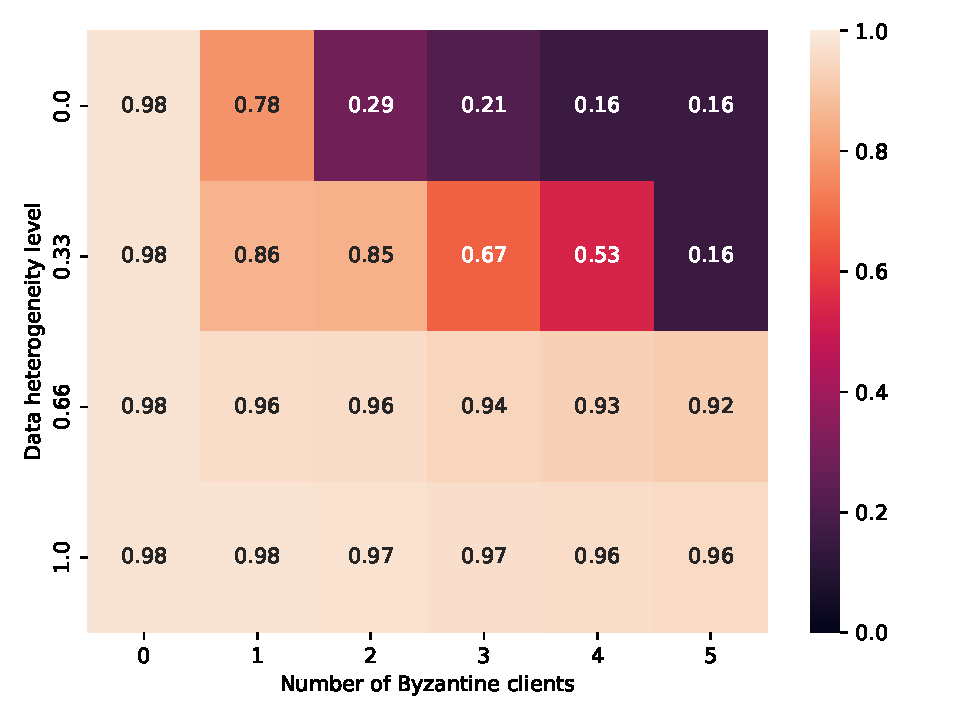
\includegraphics[width=\textwidth]{../plots/mnist_clipping_heatmaps/cnn_mnist_clipping_2/test_mnist_cnn_mnist_clipping_2_gamma_similarity_niid_NNM_ARC_CenteredClipping_nb_honest_clients_10_tolerated_f_equal_real.pdf}
        \caption{CNN ReLU (Clip $=2$)}
        \label{fig:cc_worst_case_clip2}
    \end{subfigure}
    \vspace{0.3cm}
    \begin{subfigure}[b]{0.24\textwidth}
        \centering
        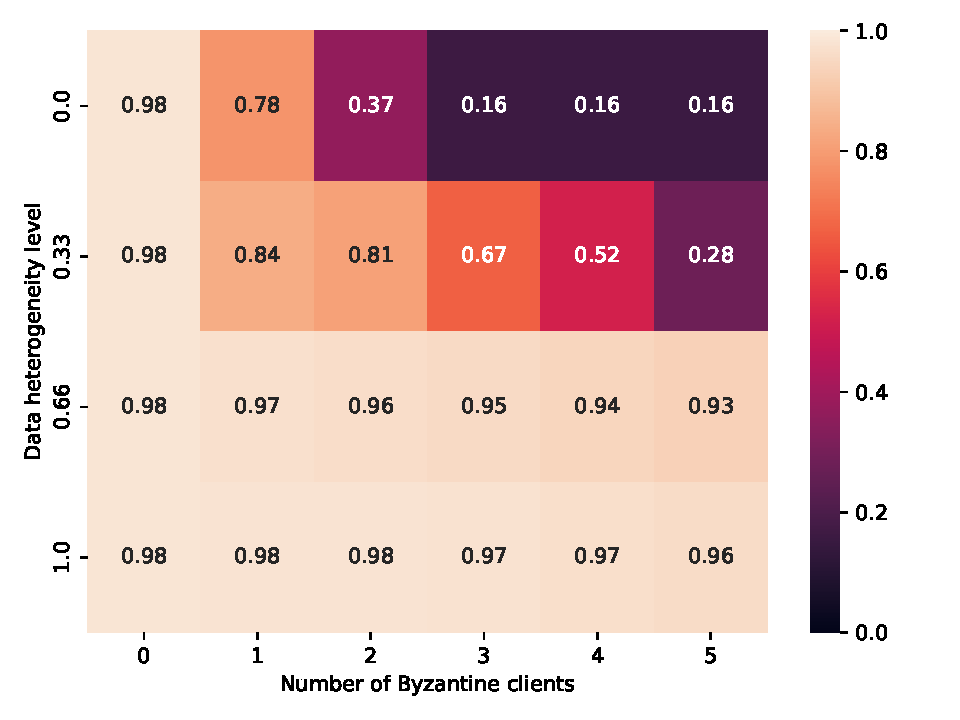
\includegraphics[width=\textwidth]{../plots/mnist_clipping_heatmaps/cnn_mnist_clipping_4/test_mnist_cnn_mnist_clipping_4_gamma_similarity_niid_NNM_ARC_CenteredClipping_nb_honest_clients_10_tolerated_f_equal_real.pdf}
        \caption{CNN ReLU (Clip $=4$)}
        \label{fig:cc_worst_case_clip4}
    \end{subfigure}
    \hfill
    \begin{subfigure}[b]{0.24\textwidth}
        \centering
        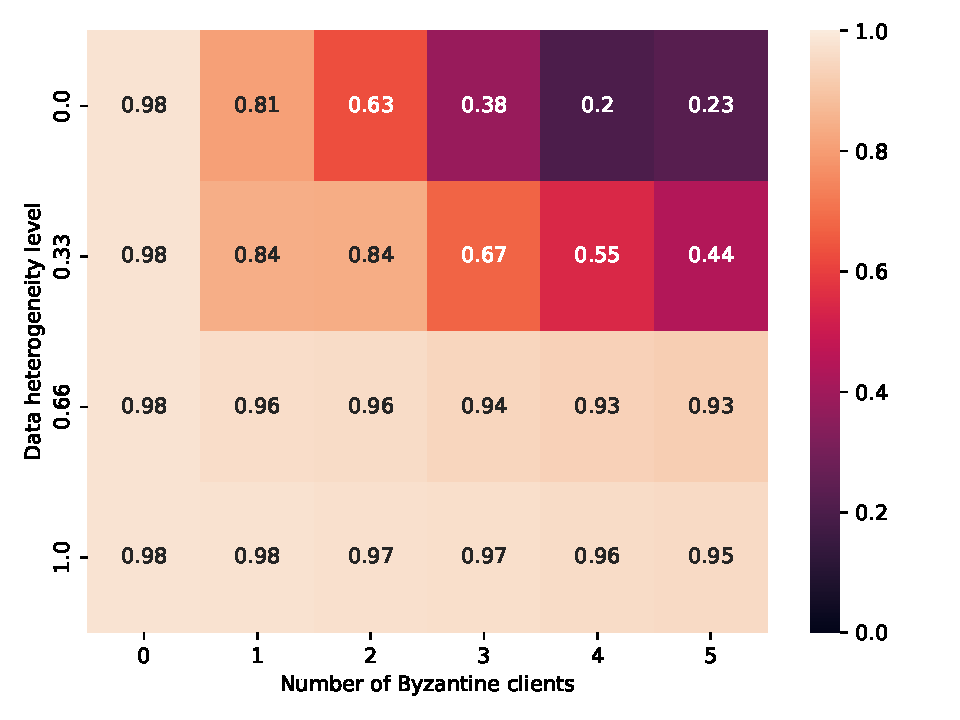
\includegraphics[width=\textwidth]{../plots/cnn_tanh_heatmaps/test_mnist_cnn_mnist_tanh_gamma_similarity_niid_NNM_ARC_CenteredClipping_nb_honest_clients_10_tolerated_f_equal_real.pdf}
        \caption{CNN Tanh}
        \label{fig:cc_worst_case_tanh}
    \end{subfigure}
    \caption{Centered Clipping (CC) under Worst-Case across all Attacks.}
    \label{fig:cc_worst_case_grid}
\end{figure}
\clearpage
\subsubsection{CC under ALIE}
\begin{figure}[htbp]
    \centering
    \begin{subfigure}[b]{0.24\textwidth}
        \centering
        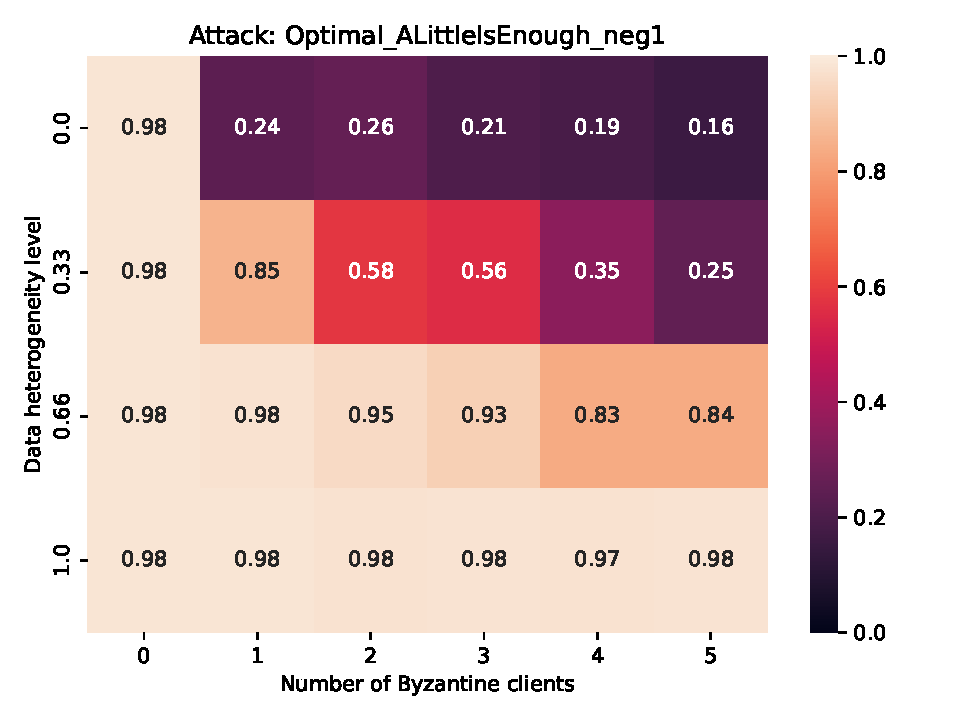
\includegraphics[width=\textwidth]{../plots/mnist_clipping_heatmaps/cnn_mnist/test_Optimal_ALittleIsEnough_neg1_mnist_cnn_mnist_gamma_similarity_niid_NNM_ARC_CenteredClipping_nb_honest_clients_10_tolerated_f_equal_real.pdf}
        \caption{CNN ReLU (No Clip)}
        \label{fig:cc_alie_noclip}
    \end{subfigure}
    \hfill
    \begin{subfigure}[b]{0.24\textwidth}
        \centering
        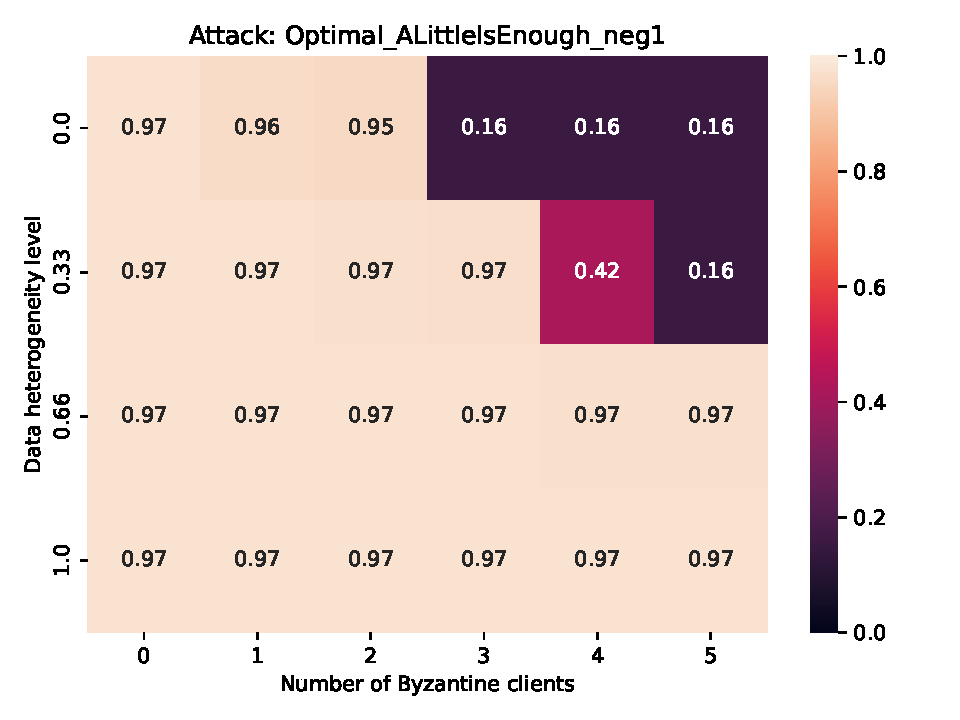
\includegraphics[width=\textwidth]{../plots/mnist_clipping_heatmaps/cnn_mnist_clipping_1/test_Optimal_ALittleIsEnough_neg1_mnist_cnn_mnist_clipping_1_gamma_similarity_niid_NNM_ARC_CenteredClipping_nb_honest_clients_10_tolerated_f_equal_real.pdf}
        \caption{CNN ReLU (Clip $=1$)}
        \label{fig:cc_alie_clip1}
    \end{subfigure}
    \hfill
    \begin{subfigure}[b]{0.24\textwidth}
        \centering
        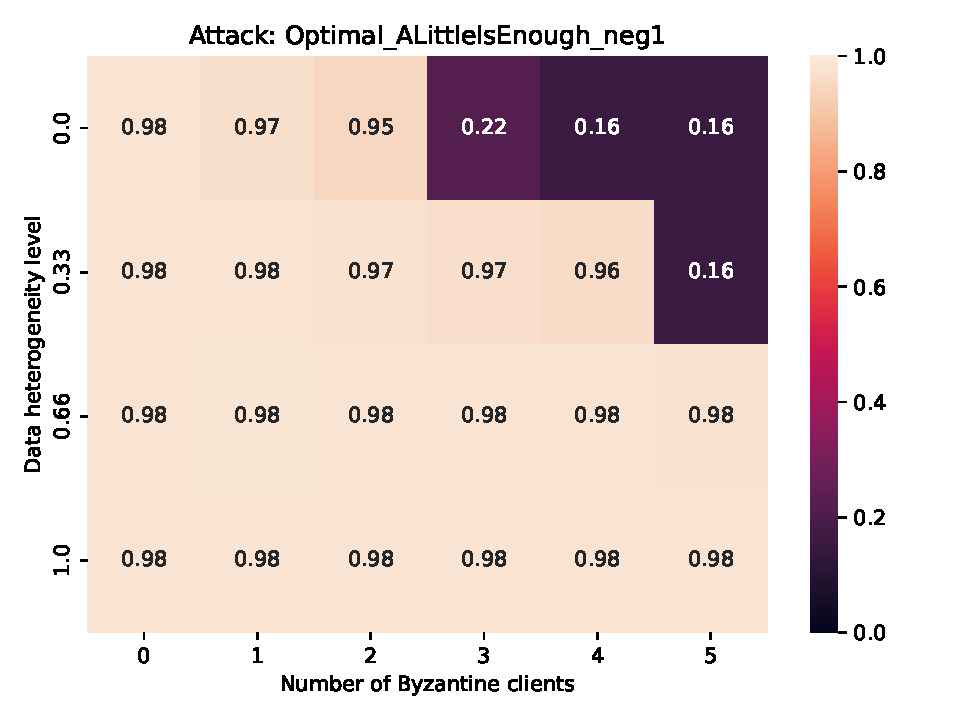
\includegraphics[width=\textwidth]{../plots/mnist_clipping_heatmaps/cnn_mnist_clipping_2/test_Optimal_ALittleIsEnough_neg1_mnist_cnn_mnist_clipping_2_gamma_similarity_niid_NNM_ARC_CenteredClipping_nb_honest_clients_10_tolerated_f_equal_real.pdf}
        \caption{CNN ReLU (Clip $=2$)}
        \label{fig:cc_alie_clip2}
    \end{subfigure}
    \vspace{0.3cm}
    \begin{subfigure}[b]{0.24\textwidth}
        \centering
        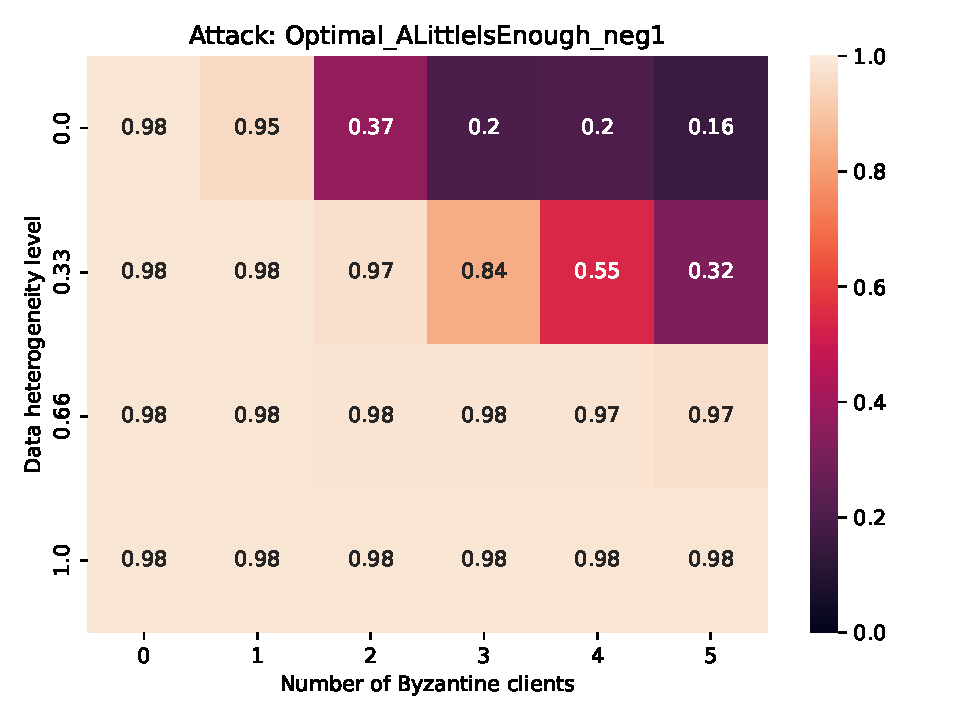
\includegraphics[width=\textwidth]{../plots/mnist_clipping_heatmaps/cnn_mnist_clipping_4/test_Optimal_ALittleIsEnough_neg1_mnist_cnn_mnist_clipping_4_gamma_similarity_niid_NNM_ARC_CenteredClipping_nb_honest_clients_10_tolerated_f_equal_real.pdf}
        \caption{CNN ReLU (Clip $=4$)}
        \label{fig:cc_alie_clip4}
    \end{subfigure}
    \hfill
    \begin{subfigure}[b]{0.24\textwidth}
        \centering
        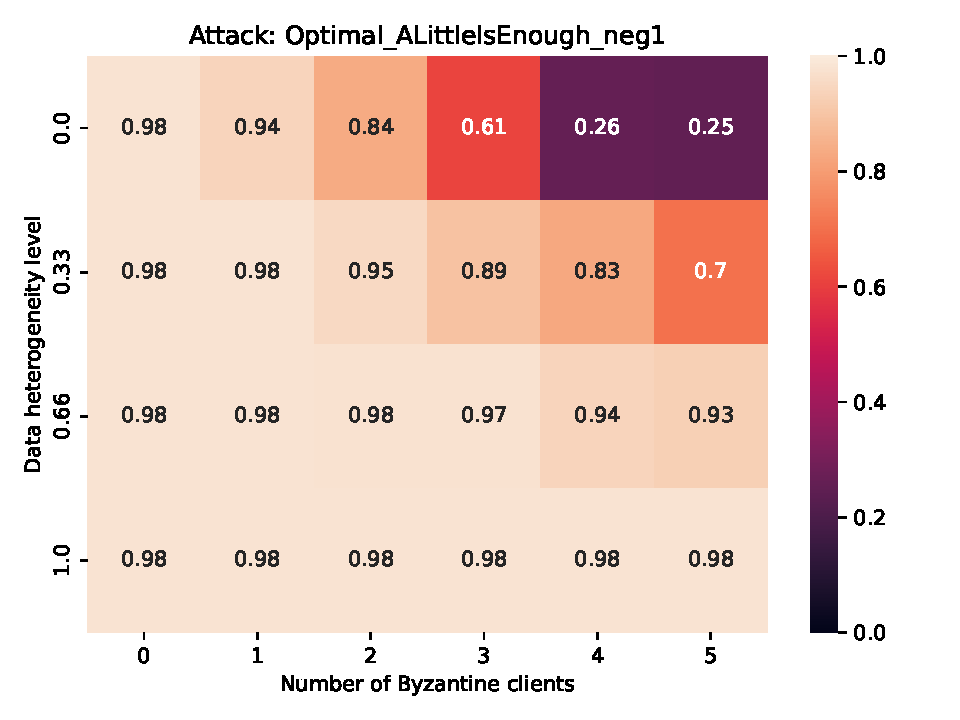
\includegraphics[width=\textwidth]{../plots/cnn_tanh_heatmaps/test_Optimal_ALittleIsEnough_neg1_mnist_cnn_mnist_tanh_gamma_similarity_niid_NNM_ARC_CenteredClipping_nb_honest_clients_10_tolerated_f_equal_real.pdf}
        \caption{CNN Tanh}
        \label{fig:cc_alie_tanh}
    \end{subfigure}
    \caption{Centered Clipping (CC) under Optimal ALIE Attack.}
    \label{fig:cc_alie_grid}
\end{figure}
\clearpage
\subsubsection{CC under SF}
\begin{figure}[htbp]
    \centering
    \begin{subfigure}[b]{0.24\textwidth}
        \centering
        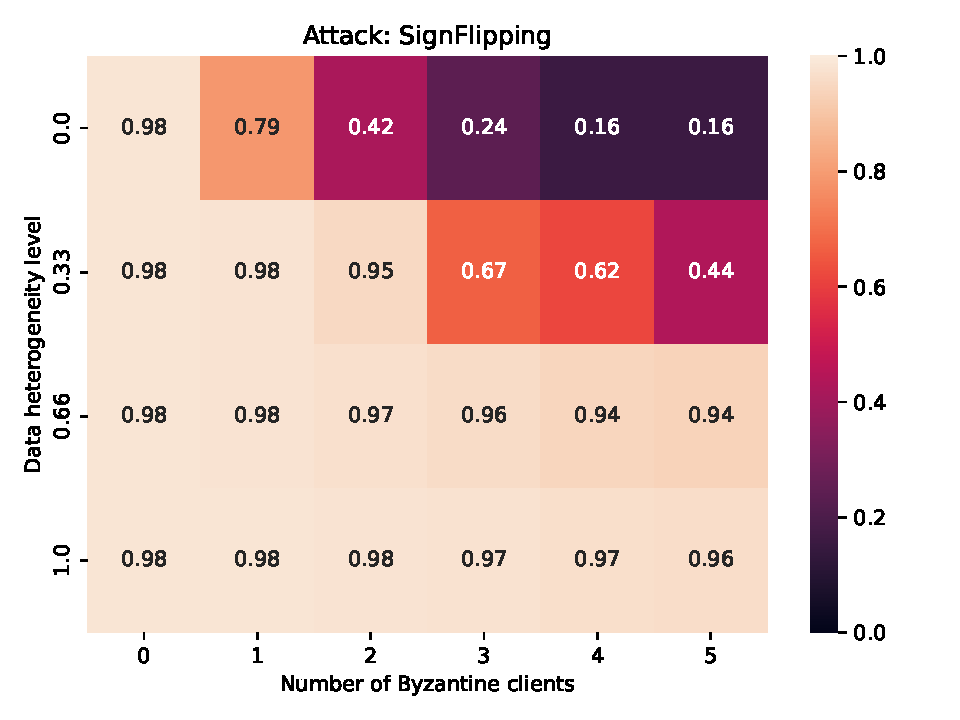
\includegraphics[width=\textwidth]{../plots/mnist_clipping_heatmaps/cnn_mnist/test_SignFlipping_mnist_cnn_mnist_gamma_similarity_niid_NNM_ARC_CenteredClipping_nb_honest_clients_10_tolerated_f_equal_real.pdf}
        \caption{CNN ReLU (No Clip)}
        \label{fig:cc_sf_noclip}
    \end{subfigure}
    \hfill
    \begin{subfigure}[b]{0.24\textwidth}
        \centering
        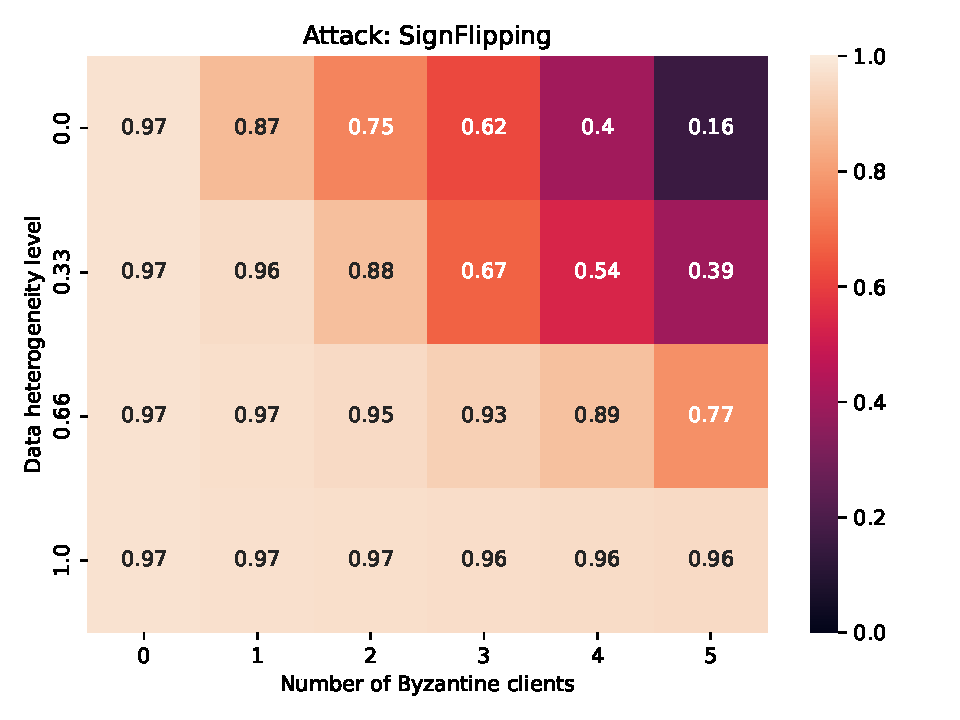
\includegraphics[width=\textwidth]{../plots/mnist_clipping_heatmaps/cnn_mnist_clipping_1/test_SignFlipping_mnist_cnn_mnist_clipping_1_gamma_similarity_niid_NNM_ARC_CenteredClipping_nb_honest_clients_10_tolerated_f_equal_real.pdf}
        \caption{CNN ReLU (Clip $=1$)}
        \label{fig:cc_sf_clip1}
    \end{subfigure}
    \hfill
    \begin{subfigure}[b]{0.24\textwidth}
        \centering
        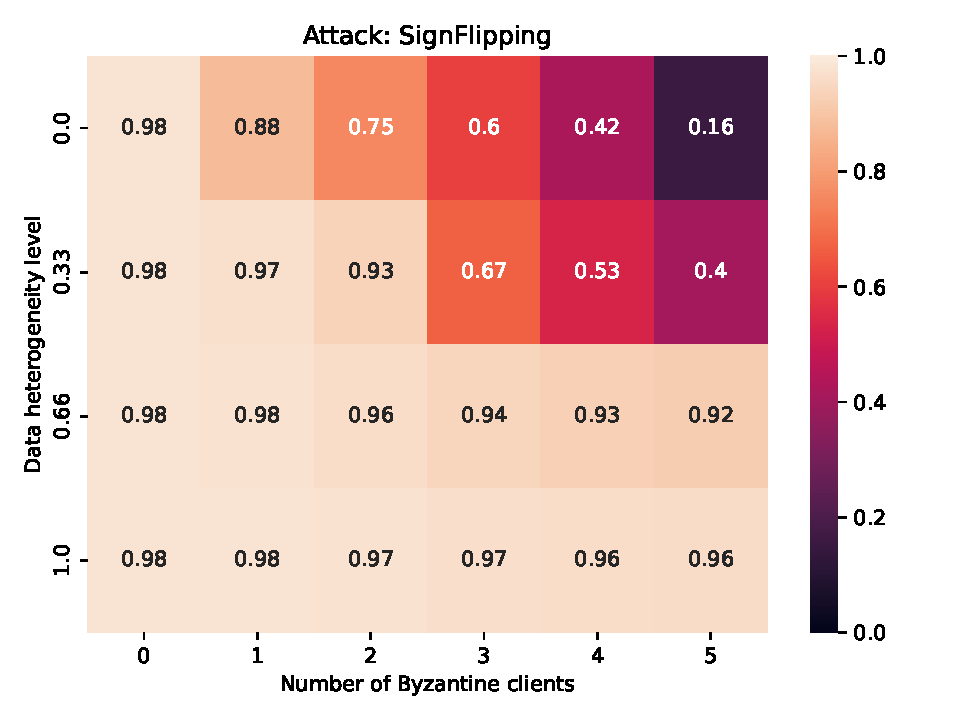
\includegraphics[width=\textwidth]{../plots/mnist_clipping_heatmaps/cnn_mnist_clipping_2/test_SignFlipping_mnist_cnn_mnist_clipping_2_gamma_similarity_niid_NNM_ARC_CenteredClipping_nb_honest_clients_10_tolerated_f_equal_real.pdf}
        \caption{CNN ReLU (Clip $=2$)}
        \label{fig:cc_sf_clip2}
    \end{subfigure}
    \vspace{0.3cm}
    \begin{subfigure}[b]{0.24\textwidth}
        \centering
        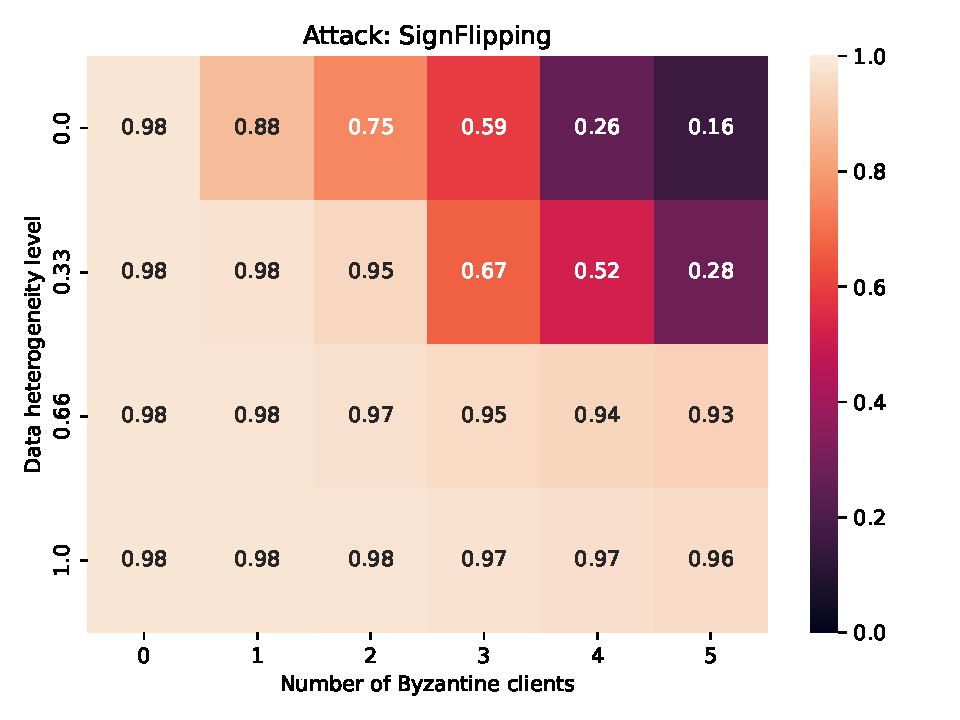
\includegraphics[width=\textwidth]{../plots/mnist_clipping_heatmaps/cnn_mnist_clipping_4/test_SignFlipping_mnist_cnn_mnist_clipping_4_gamma_similarity_niid_NNM_ARC_CenteredClipping_nb_honest_clients_10_tolerated_f_equal_real.pdf}
        \caption{CNN ReLU (Clip $=4$)}
        \label{fig:cc_sf_clip4}
    \end{subfigure}
    \hfill
    \begin{subfigure}[b]{0.24\textwidth}
        \centering
        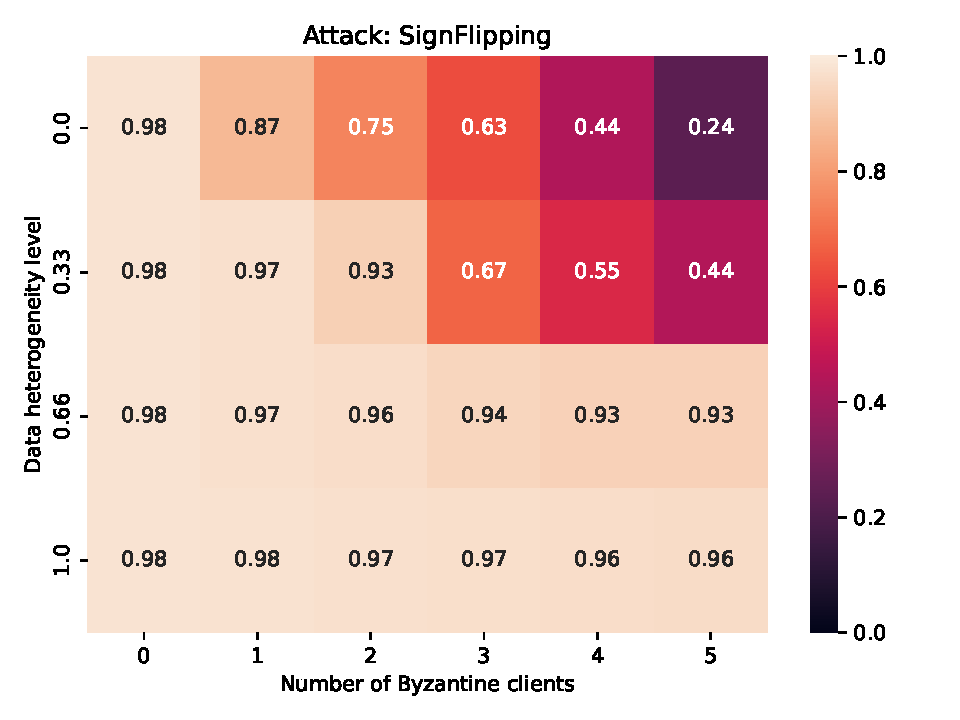
\includegraphics[width=\textwidth]{../plots/cnn_tanh_heatmaps/test_SignFlipping_mnist_cnn_mnist_tanh_gamma_similarity_niid_NNM_ARC_CenteredClipping_nb_honest_clients_10_tolerated_f_equal_real.pdf}
        \caption{CNN Tanh}
        \label{fig:cc_sf_tanh}
    \end{subfigure}
    \caption{Centered Clipping (CC) under Sign Flipping Attack.}
    \label{fig:cc_sf_grid}
\end{figure}
\clearpage
\subsubsection{CC under IPM}
\begin{figure}[htbp]
    \centering
    \begin{subfigure}[b]{0.24\textwidth}
        \centering
        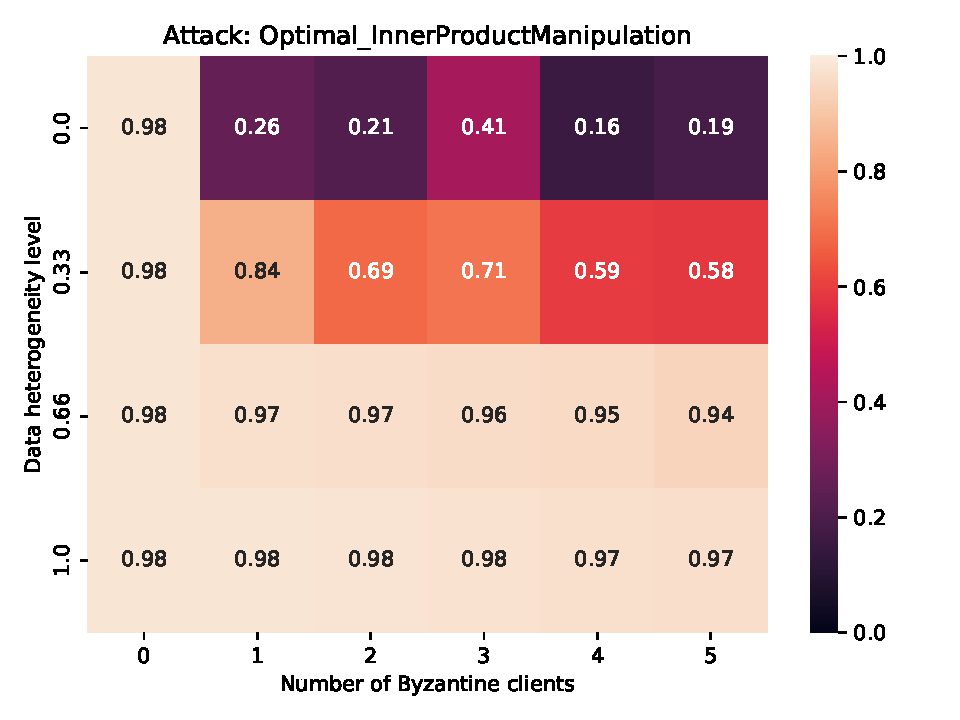
\includegraphics[width=\textwidth]{../plots/mnist_clipping_heatmaps/cnn_mnist/test_Optimal_InnerProductManipulation_mnist_cnn_mnist_gamma_similarity_niid_NNM_ARC_CenteredClipping_nb_honest_clients_10_tolerated_f_equal_real.pdf}
        \caption{CNN ReLU (No Clip)}
        \label{fig:cc_ipm_noclip}
    \end{subfigure}
    \hfill
    \begin{subfigure}[b]{0.24\textwidth}
        \centering
        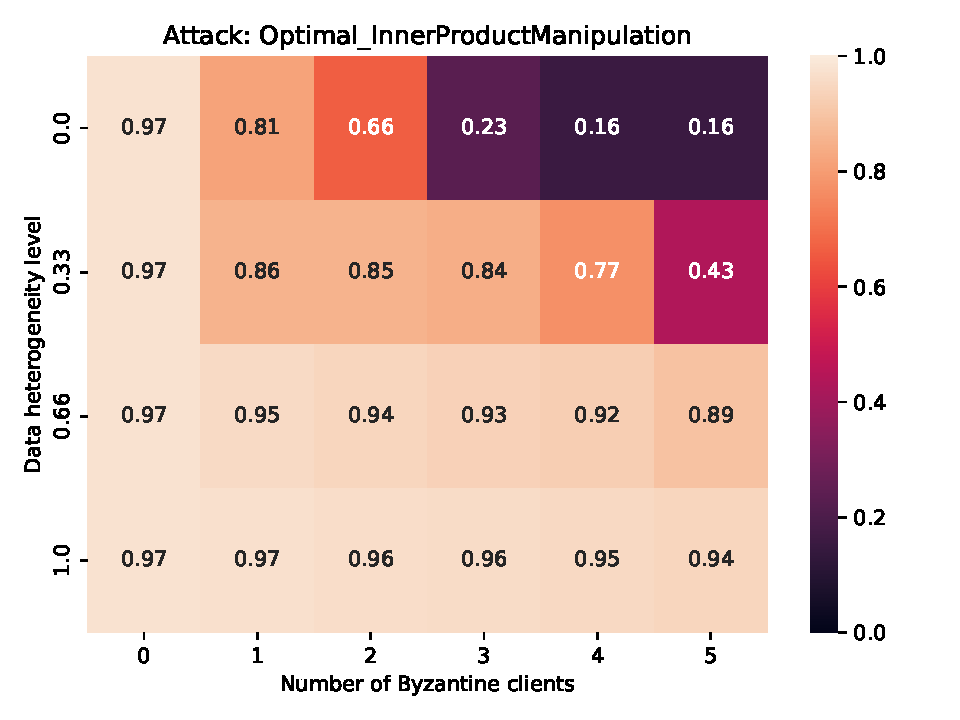
\includegraphics[width=\textwidth]{../plots/mnist_clipping_heatmaps/cnn_mnist_clipping_1/test_Optimal_InnerProductManipulation_mnist_cnn_mnist_clipping_1_gamma_similarity_niid_NNM_ARC_CenteredClipping_nb_honest_clients_10_tolerated_f_equal_real.pdf}
        \caption{CNN ReLU (Clip $=1$)}
        \label{fig:cc_ipm_clip1}
    \end{subfigure}
    \hfill
    \begin{subfigure}[b]{0.24\textwidth}
        \centering
        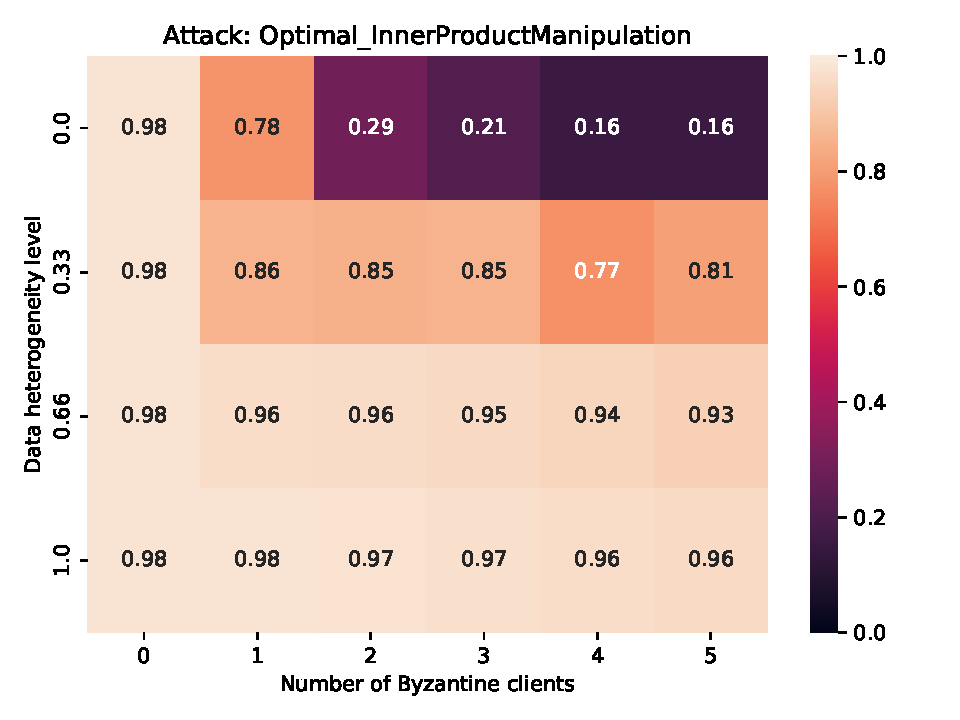
\includegraphics[width=\textwidth]{../plots/mnist_clipping_heatmaps/cnn_mnist_clipping_2/test_Optimal_InnerProductManipulation_mnist_cnn_mnist_clipping_2_gamma_similarity_niid_NNM_ARC_CenteredClipping_nb_honest_clients_10_tolerated_f_equal_real.pdf}
        \caption{CNN ReLU (Clip $=2$)}
        \label{fig:cc_ipm_clip2}
    \end{subfigure}
    \vspace{0.3cm}
    \begin{subfigure}[b]{0.24\textwidth}
        \centering
        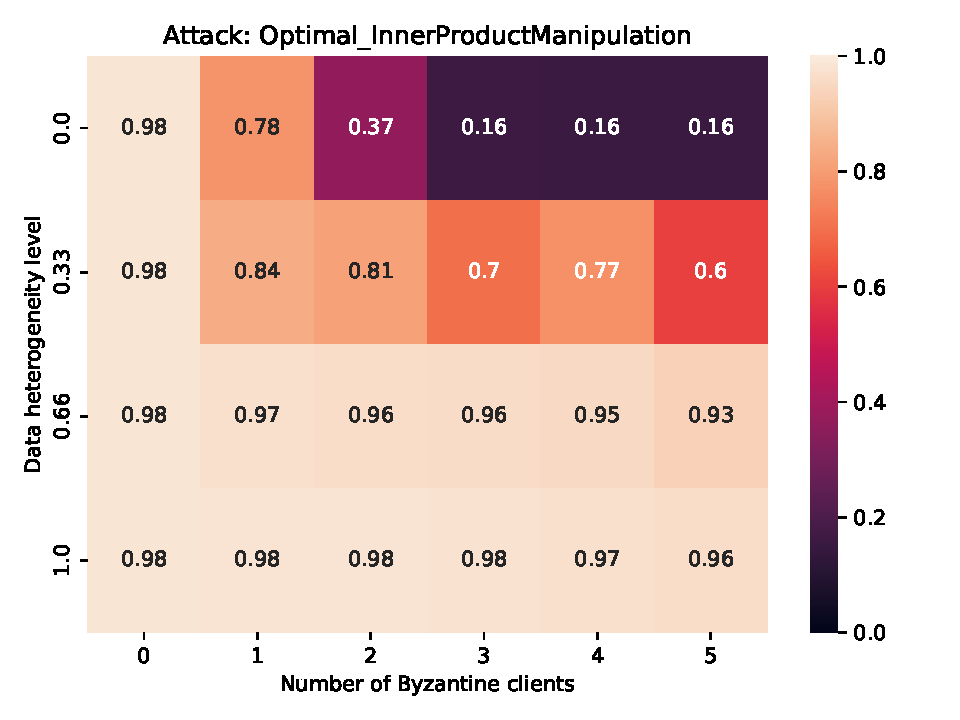
\includegraphics[width=\textwidth]{../plots/mnist_clipping_heatmaps/cnn_mnist_clipping_4/test_Optimal_InnerProductManipulation_mnist_cnn_mnist_clipping_4_gamma_similarity_niid_NNM_ARC_CenteredClipping_nb_honest_clients_10_tolerated_f_equal_real.pdf}
        \caption{CNN ReLU (Clip $=4$)}
        \label{fig:cc_ipm_clip4}
    \end{subfigure}
    \hfill
    \begin{subfigure}[b]{0.24\textwidth}
        \centering
        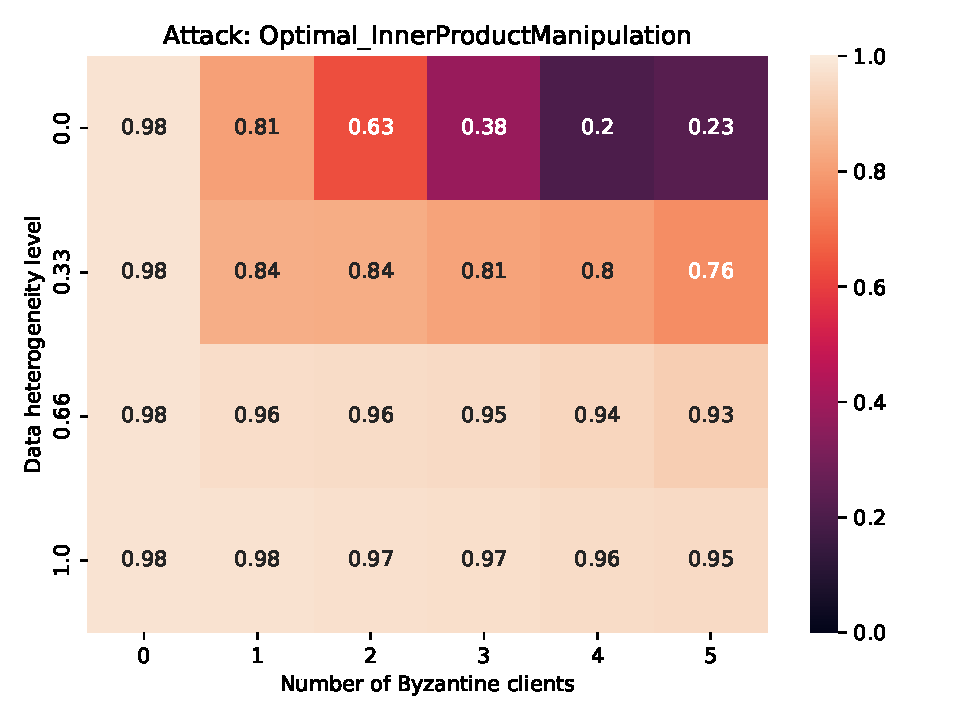
\includegraphics[width=\textwidth]{../plots/cnn_tanh_heatmaps/test_Optimal_InnerProductManipulation_mnist_cnn_mnist_tanh_gamma_similarity_niid_NNM_ARC_CenteredClipping_nb_honest_clients_10_tolerated_f_equal_real.pdf}
        \caption{CNN Tanh}
        \label{fig:cc_ipm_tanh}
    \end{subfigure}
    \caption{Centered Clipping (CC) under Optimal IPM Attack.}
    \label{fig:cc_ipm_grid}
\end{figure}
\clearpage
\subsection{Geometric Median (GM)}
\subsubsection{GM under Worst-Case across all Attacks}
\begin{figure}[htbp]
    \centering
    \begin{subfigure}[b]{0.24\textwidth}
        \centering
        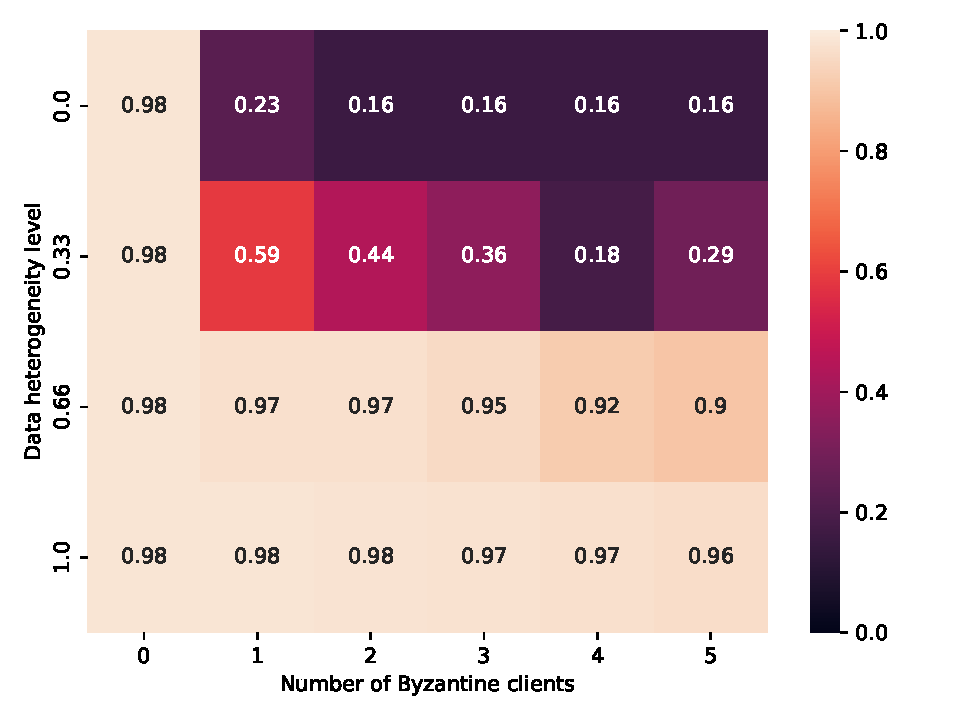
\includegraphics[width=\textwidth]{../plots/mnist_clipping_heatmaps/cnn_mnist/test_mnist_cnn_mnist_gamma_similarity_niid_NNM_ARC_GeometricMedian_nb_honest_clients_10_tolerated_f_equal_real.pdf}
        \caption{CNN ReLU (No Clip)}
        \label{fig:gm_worst_case_noclip}
    \end{subfigure}
    \hfill
    \begin{subfigure}[b]{0.24\textwidth}
        \centering
        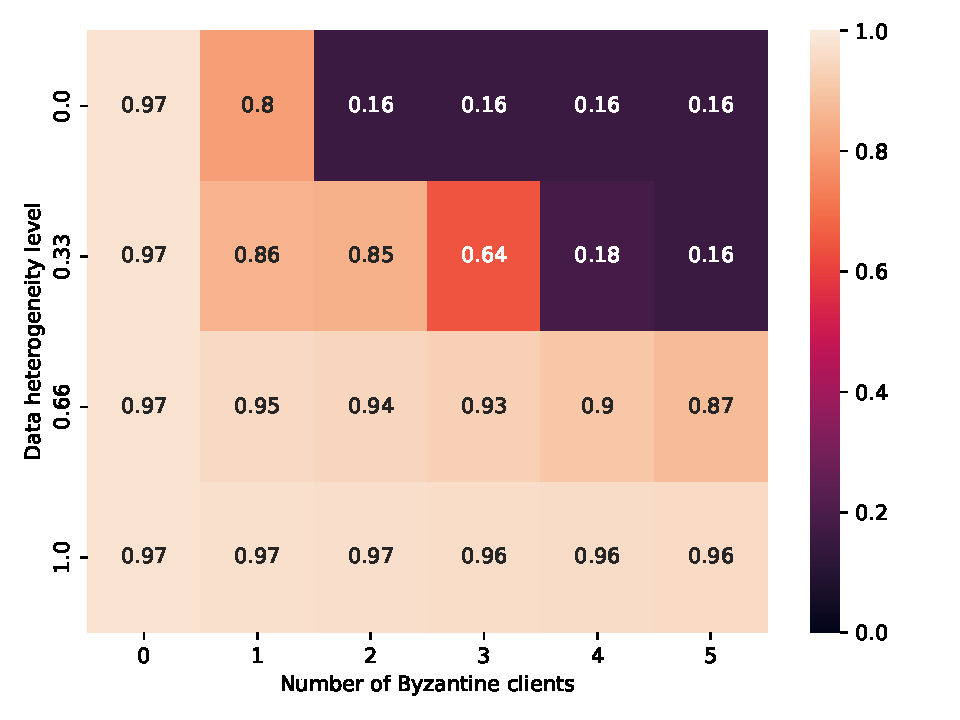
\includegraphics[width=\textwidth]{../plots/mnist_clipping_heatmaps/cnn_mnist_clipping_1/test_mnist_cnn_mnist_clipping_1_gamma_similarity_niid_NNM_ARC_GeometricMedian_nb_honest_clients_10_tolerated_f_equal_real.pdf}
        \caption{CNN ReLU (Clip $=1$)}
        \label{fig:gm_worst_case_clip1}
    \end{subfigure}
    \hfill
    \begin{subfigure}[b]{0.24\textwidth}
        \centering
        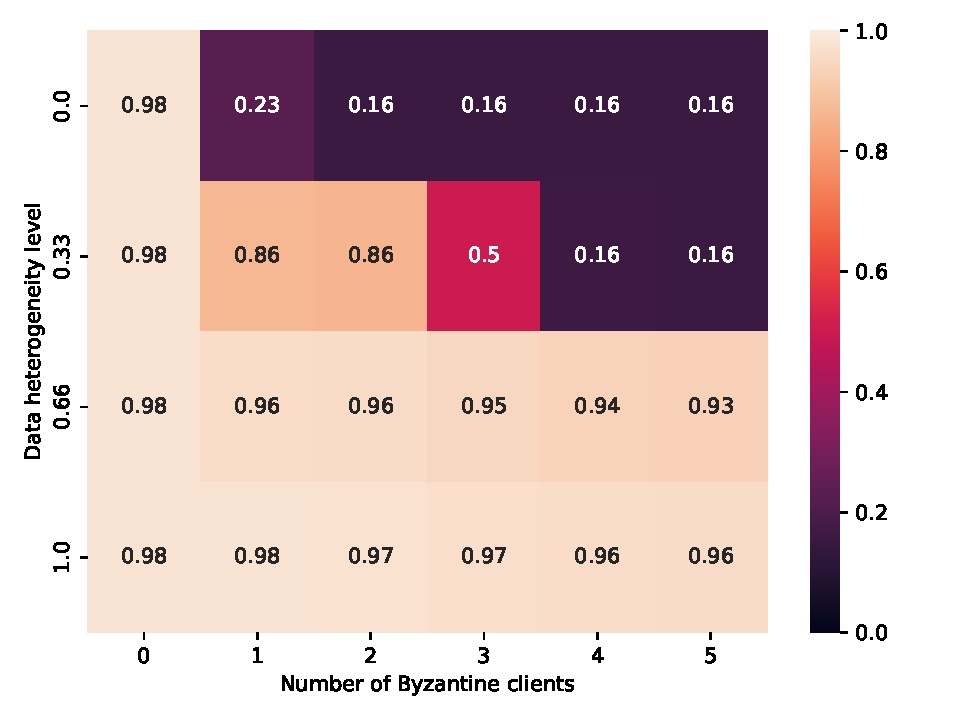
\includegraphics[width=\textwidth]{../plots/mnist_clipping_heatmaps/cnn_mnist_clipping_2/test_mnist_cnn_mnist_clipping_2_gamma_similarity_niid_NNM_ARC_GeometricMedian_nb_honest_clients_10_tolerated_f_equal_real.pdf}
        \caption{CNN ReLU (Clip $=2$)}
        \label{fig:gm_worst_case_clip2}
    \end{subfigure}
    \vspace{0.3cm}
    \begin{subfigure}[b]{0.24\textwidth}
        \centering
        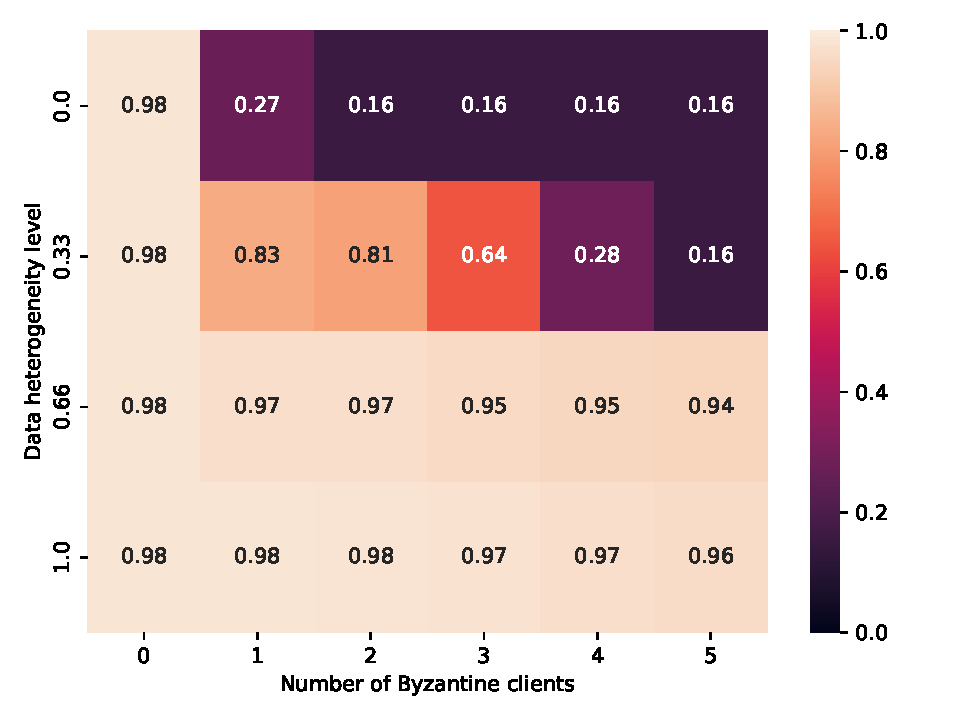
\includegraphics[width=\textwidth]{../plots/mnist_clipping_heatmaps/cnn_mnist_clipping_4/test_mnist_cnn_mnist_clipping_4_gamma_similarity_niid_NNM_ARC_GeometricMedian_nb_honest_clients_10_tolerated_f_equal_real.pdf}
        \caption{CNN ReLU (Clip $=4$)}
        \label{fig:gm_worst_case_clip4}
    \end{subfigure}
    \hfill
    \begin{subfigure}[b]{0.24\textwidth}
        \centering
        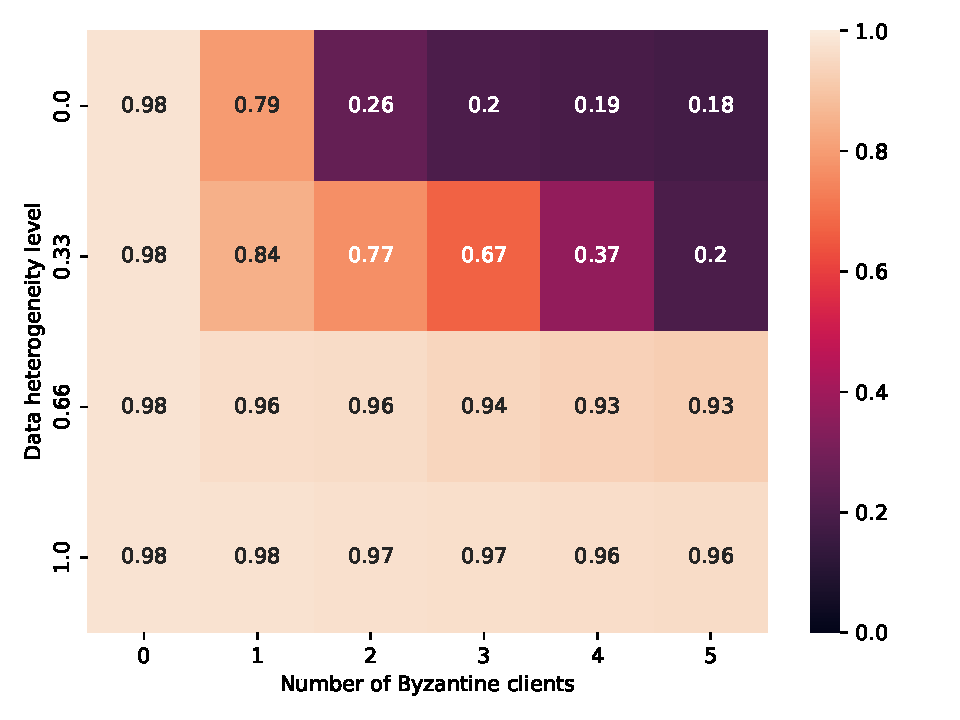
\includegraphics[width=\textwidth]{../plots/cnn_tanh_heatmaps/test_mnist_cnn_mnist_tanh_gamma_similarity_niid_NNM_ARC_GeometricMedian_nb_honest_clients_10_tolerated_f_equal_real.pdf}
        \caption{CNN Tanh}
        \label{fig:gm_worst_case_tanh}
    \end{subfigure}
    \hfill
    \begin{subfigure}[b]{0.24\textwidth}
        \centering
        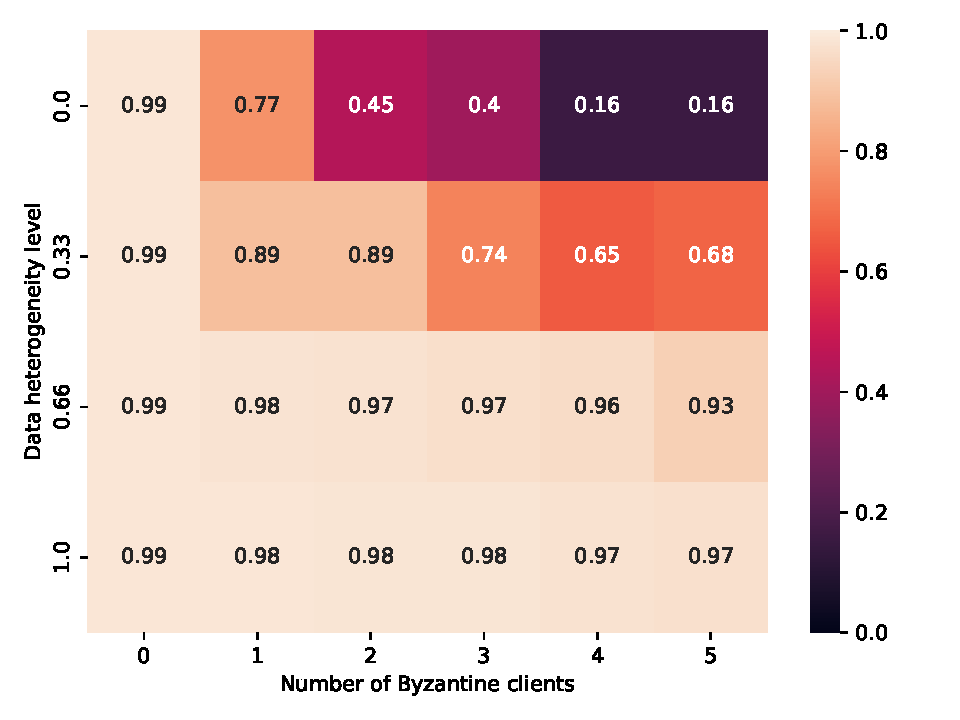
\includegraphics[width=\textwidth]{../plots/cnn_clipped_heatmaps/test_mnist_cnn_mnist_gamma_similarity_niid_NNM_ARC_GeometricMedian_nb_honest_clients_10_tolerated_f_equal_real.pdf}
        \caption{CNN ReLU (Grad-Norm Clip $=21$)}
        \label{fig:gm_worst_case_gradclip21}
    \end{subfigure}
    \caption{Geometric Median (GM) under Worst-Case across all Attacks.}
    \label{fig:gm_worst_case_grid}
\end{figure}
\clearpage
\subsubsection{GM under ALIE}
\begin{figure}[htbp]
    \centering
    \begin{subfigure}[b]{0.24\textwidth}
        \centering
        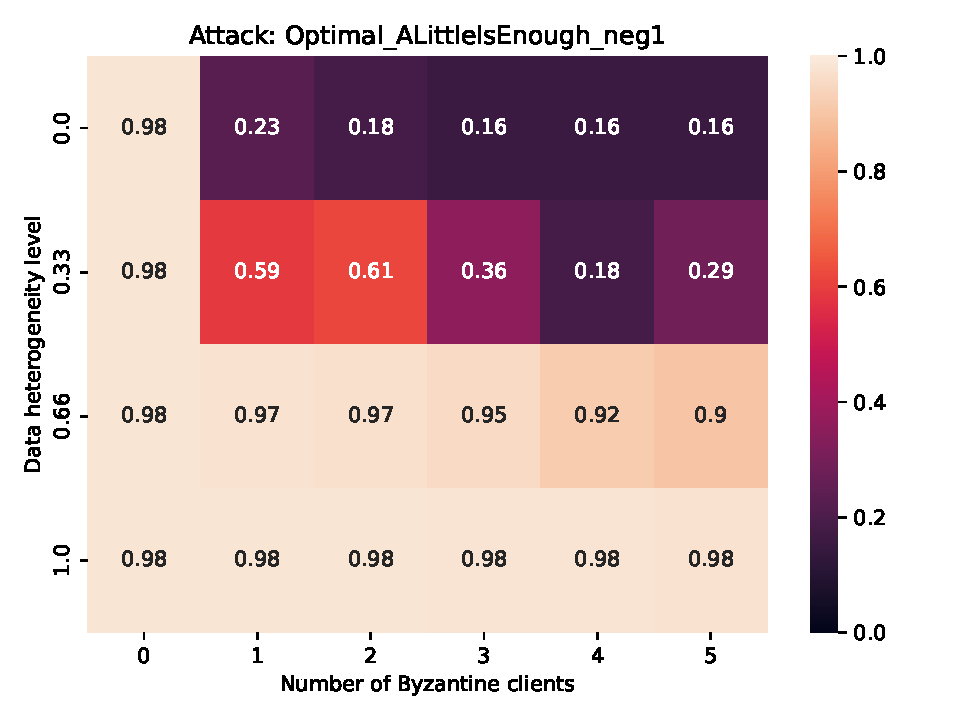
\includegraphics[width=\textwidth]{../plots/mnist_clipping_heatmaps/cnn_mnist/test_Optimal_ALittleIsEnough_neg1_mnist_cnn_mnist_gamma_similarity_niid_NNM_ARC_GeometricMedian_nb_honest_clients_10_tolerated_f_equal_real.pdf}
        \caption{CNN ReLU (No Clip)}
        \label{fig:gm_alie_noclip}
    \end{subfigure}
    \hfill
    \begin{subfigure}[b]{0.24\textwidth}
        \centering
        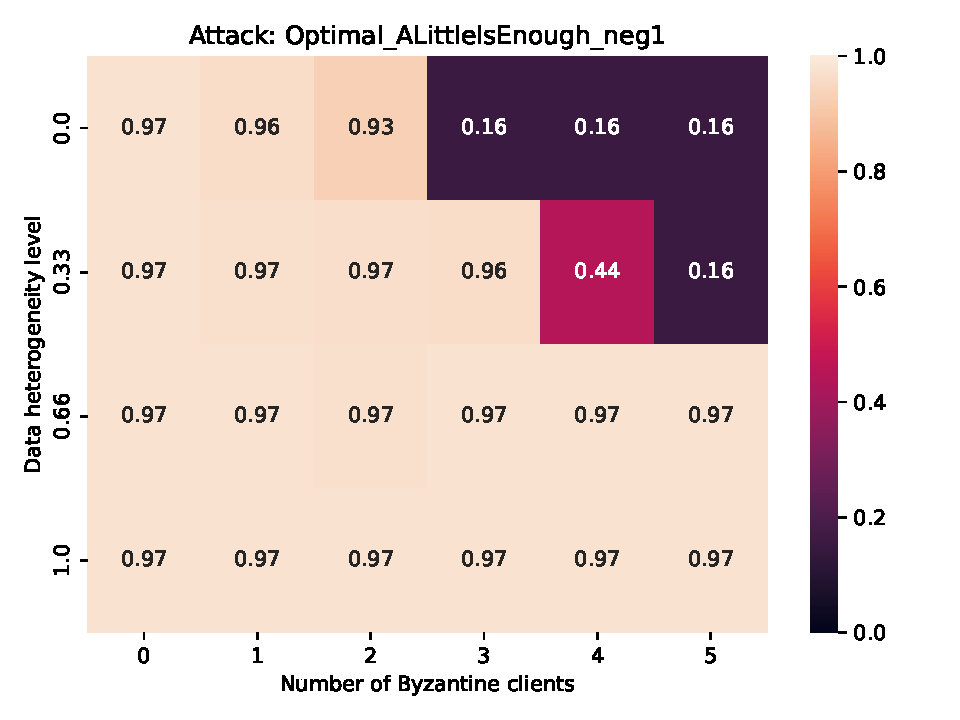
\includegraphics[width=\textwidth]{../plots/mnist_clipping_heatmaps/cnn_mnist_clipping_1/test_Optimal_ALittleIsEnough_neg1_mnist_cnn_mnist_clipping_1_gamma_similarity_niid_NNM_ARC_GeometricMedian_nb_honest_clients_10_tolerated_f_equal_real.pdf}
        \caption{CNN ReLU (Clip $=1$)}
        \label{fig:gm_alie_clip1}
    \end{subfigure}
    \hfill
    \begin{subfigure}[b]{0.24\textwidth}
        \centering
        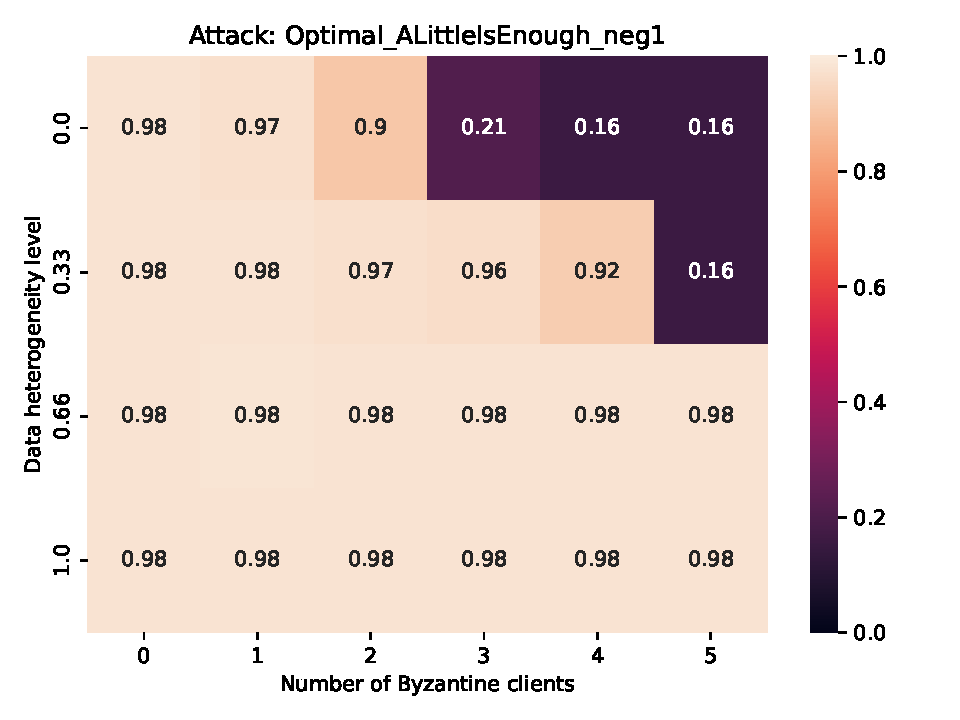
\includegraphics[width=\textwidth]{../plots/mnist_clipping_heatmaps/cnn_mnist_clipping_2/test_Optimal_ALittleIsEnough_neg1_mnist_cnn_mnist_clipping_2_gamma_similarity_niid_NNM_ARC_GeometricMedian_nb_honest_clients_10_tolerated_f_equal_real.pdf}
        \caption{CNN ReLU (Clip $=2$)}
        \label{fig:gm_alie_clip2}
    \end{subfigure}
    \vspace{0.3cm}
    \begin{subfigure}[b]{0.24\textwidth}
        \centering
        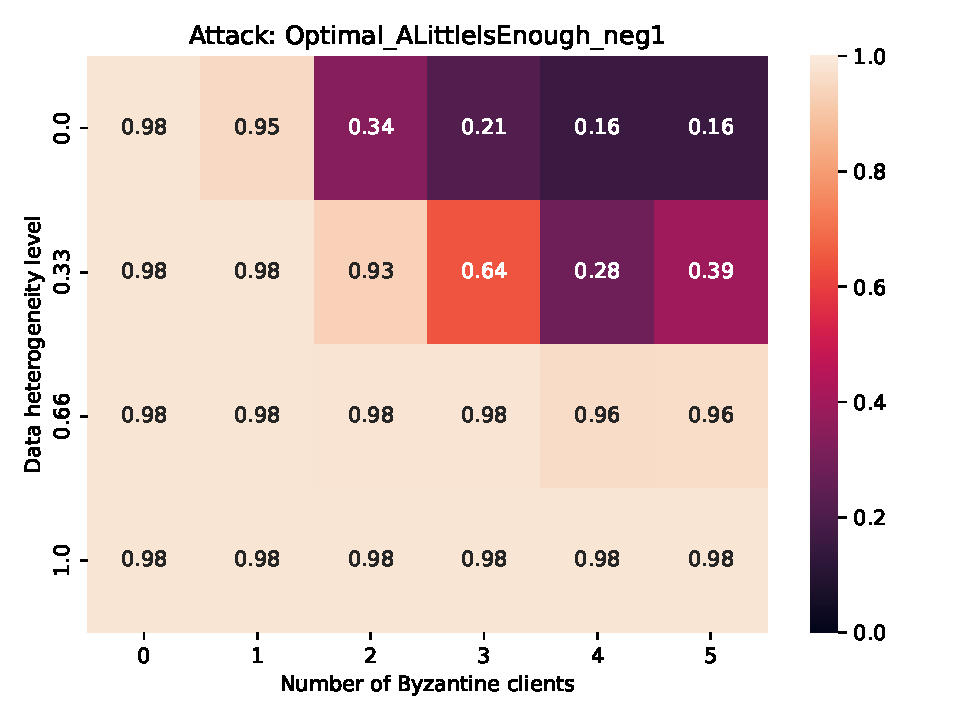
\includegraphics[width=\textwidth]{../plots/mnist_clipping_heatmaps/cnn_mnist_clipping_4/test_Optimal_ALittleIsEnough_neg1_mnist_cnn_mnist_clipping_4_gamma_similarity_niid_NNM_ARC_GeometricMedian_nb_honest_clients_10_tolerated_f_equal_real.pdf}
        \caption{CNN ReLU (Clip $=4$)}
        \label{fig:gm_alie_clip4}
    \end{subfigure}
    \hfill
    \begin{subfigure}[b]{0.24\textwidth}
        \centering
        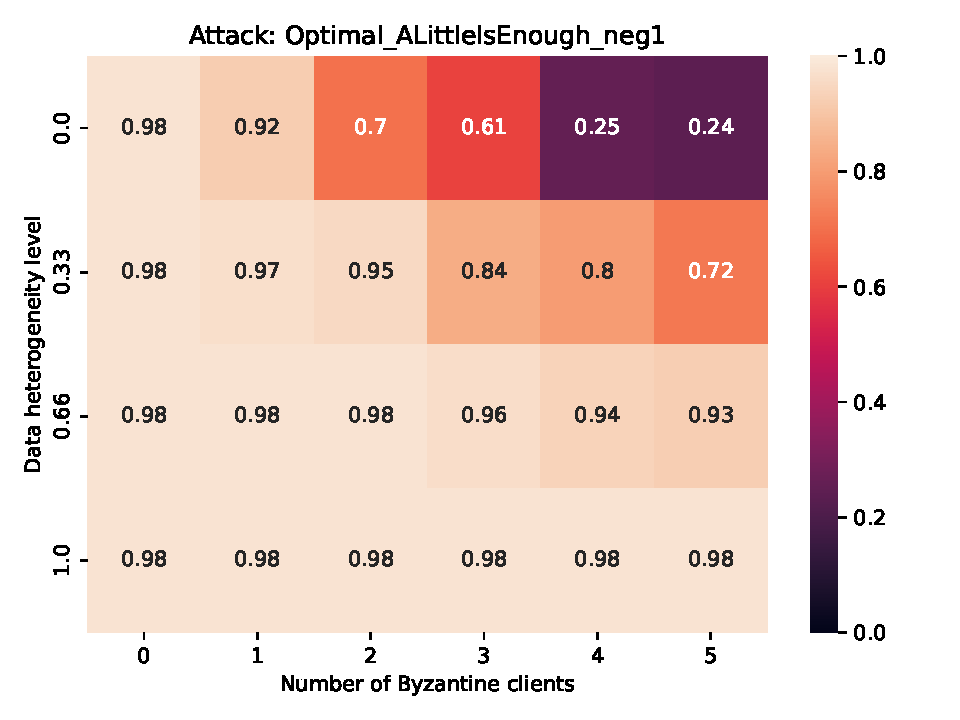
\includegraphics[width=\textwidth]{../plots/cnn_tanh_heatmaps/test_Optimal_ALittleIsEnough_neg1_mnist_cnn_mnist_tanh_gamma_similarity_niid_NNM_ARC_GeometricMedian_nb_honest_clients_10_tolerated_f_equal_real.pdf}
        \caption{CNN Tanh}
        \label{fig:gm_alie_tanh}
    \end{subfigure}
    \hfill
    \begin{subfigure}[b]{0.24\textwidth}
        \centering
        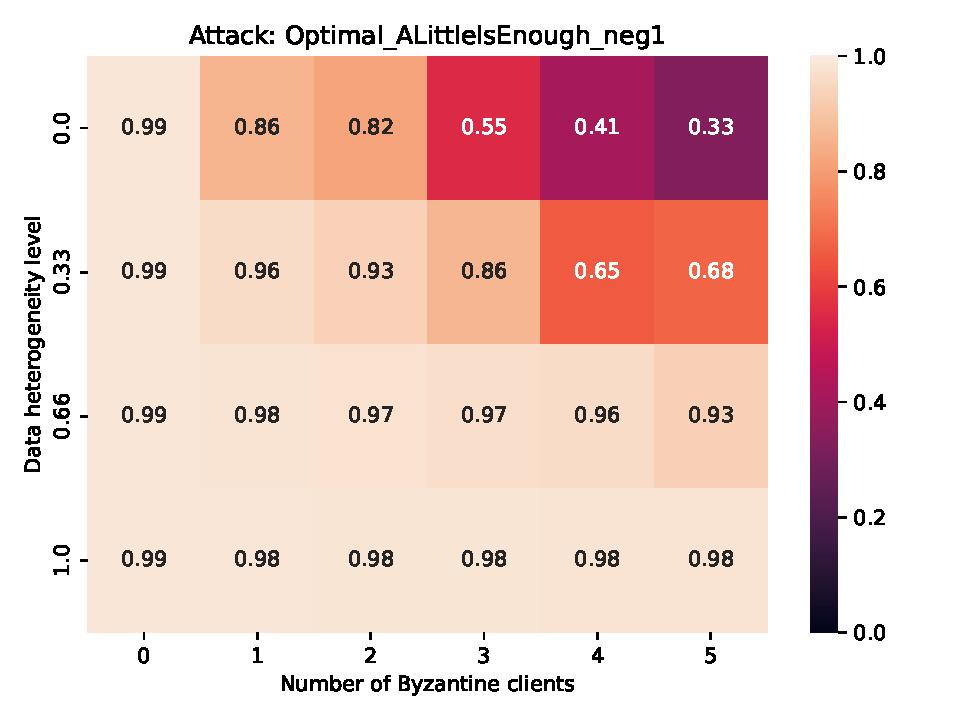
\includegraphics[width=\textwidth]{../plots/cnn_clipped_heatmaps/test_Optimal_ALittleIsEnough_neg1_mnist_cnn_mnist_gamma_similarity_niid_NNM_ARC_GeometricMedian_nb_honest_clients_10_tolerated_f_equal_real.pdf}
        \caption{CNN ReLU (Grad-Norm Clip $=21$)}
        \label{fig:gm_alie_gradclip21}
    \end{subfigure}
    \caption{Geometric Median (GM) under Optimal ALIE Attack.}
    \label{fig:gm_alie_grid}
\end{figure}
\clearpage
\subsubsection{GM under SF}
\begin{figure}[htbp]
    \centering
    \begin{subfigure}[b]{0.24\textwidth}
        \centering
        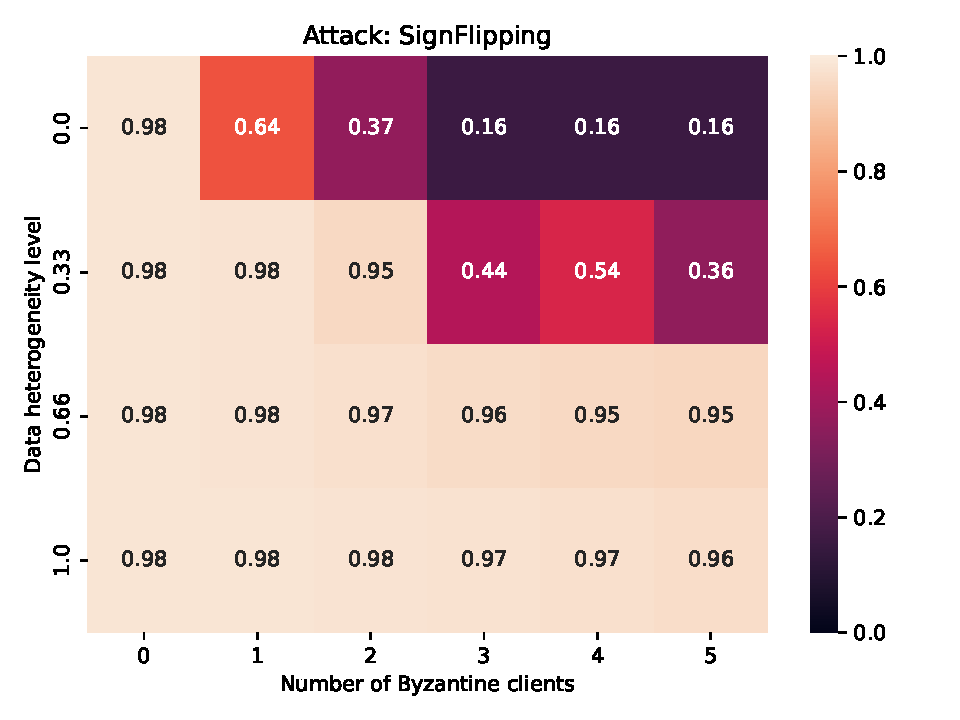
\includegraphics[width=\textwidth]{../plots/mnist_clipping_heatmaps/cnn_mnist/test_SignFlipping_mnist_cnn_mnist_gamma_similarity_niid_NNM_ARC_GeometricMedian_nb_honest_clients_10_tolerated_f_equal_real.pdf}
        \caption{CNN ReLU (No Clip)}
        \label{fig:gm_sf_noclip}
    \end{subfigure}
    \hfill
    \begin{subfigure}[b]{0.24\textwidth}
        \centering
        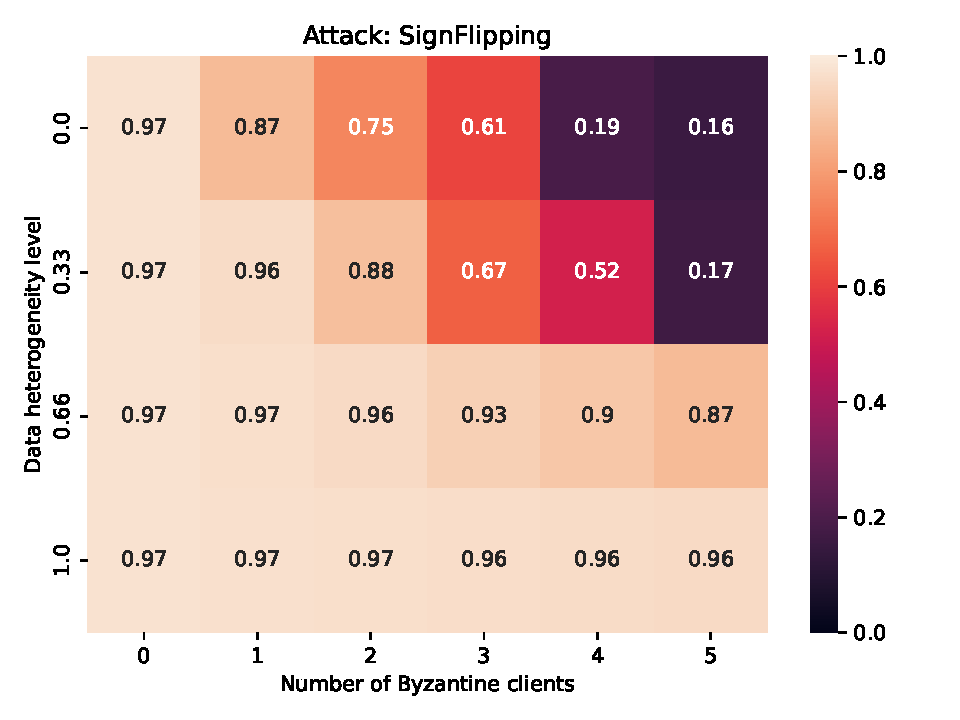
\includegraphics[width=\textwidth]{../plots/mnist_clipping_heatmaps/cnn_mnist_clipping_1/test_SignFlipping_mnist_cnn_mnist_clipping_1_gamma_similarity_niid_NNM_ARC_GeometricMedian_nb_honest_clients_10_tolerated_f_equal_real.pdf}
        \caption{CNN ReLU (Clip $=1$)}
        \label{fig:gm_sf_clip1}
    \end{subfigure}
    \hfill
    \begin{subfigure}[b]{0.24\textwidth}
        \centering
        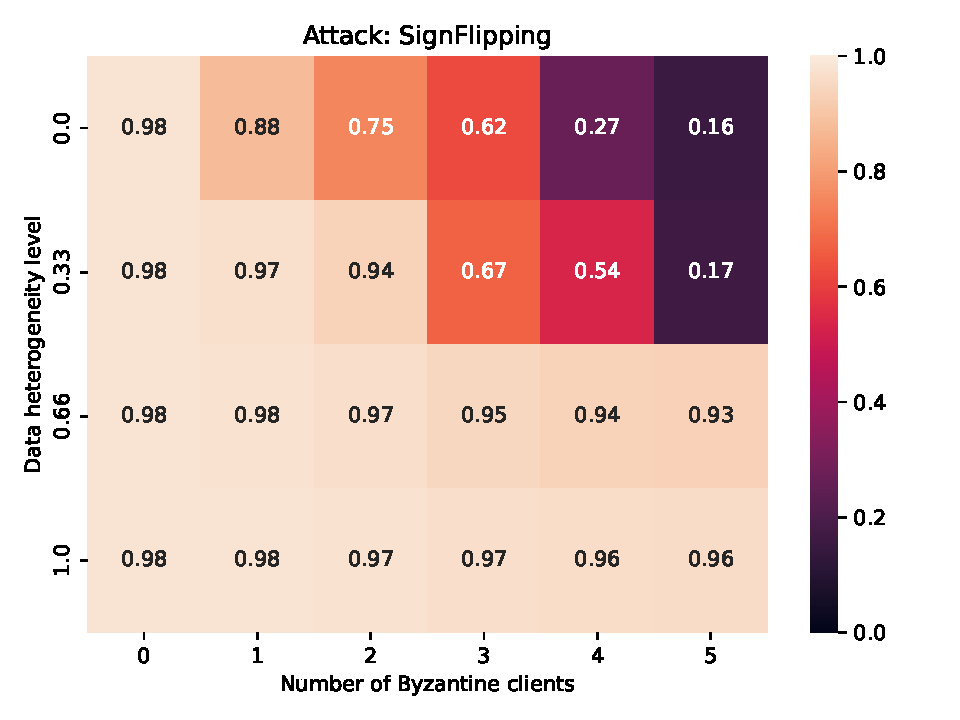
\includegraphics[width=\textwidth]{../plots/mnist_clipping_heatmaps/cnn_mnist_clipping_2/test_SignFlipping_mnist_cnn_mnist_clipping_2_gamma_similarity_niid_NNM_ARC_GeometricMedian_nb_honest_clients_10_tolerated_f_equal_real.pdf}
        \caption{CNN ReLU (Clip $=2$)}
        \label{fig:gm_sf_clip2}
    \end{subfigure}
    \vspace{0.3cm}
    \begin{subfigure}[b]{0.24\textwidth}
        \centering
        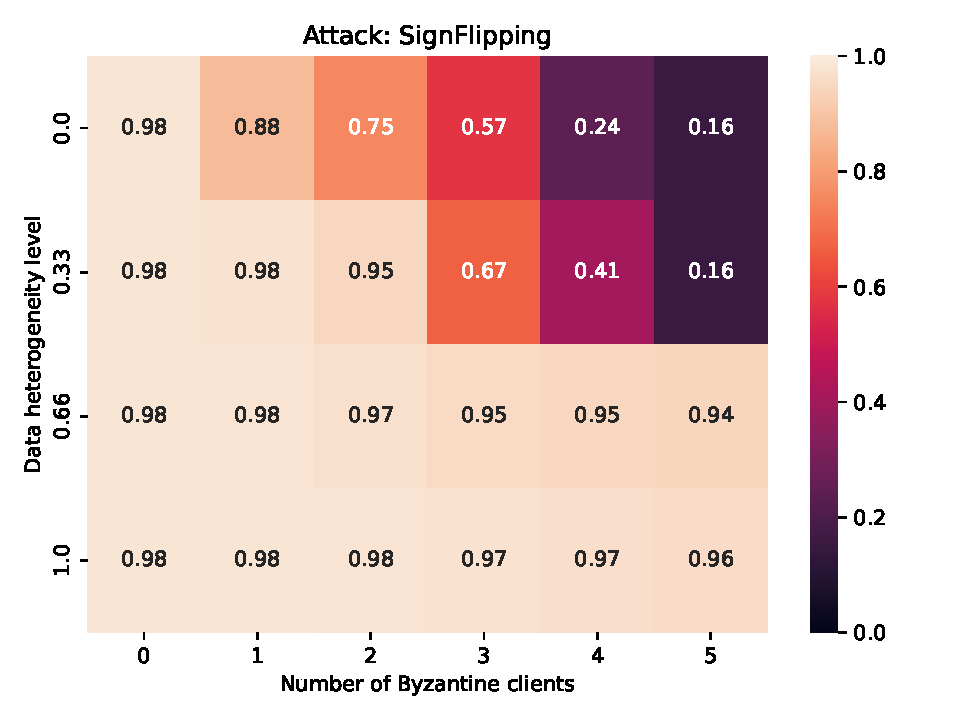
\includegraphics[width=\textwidth]{../plots/mnist_clipping_heatmaps/cnn_mnist_clipping_4/test_SignFlipping_mnist_cnn_mnist_clipping_4_gamma_similarity_niid_NNM_ARC_GeometricMedian_nb_honest_clients_10_tolerated_f_equal_real.pdf}
        \caption{CNN ReLU (Clip $=4$)}
        \label{fig:gm_sf_clip4}
    \end{subfigure}
    \hfill
    \begin{subfigure}[b]{0.24\textwidth}
        \centering
        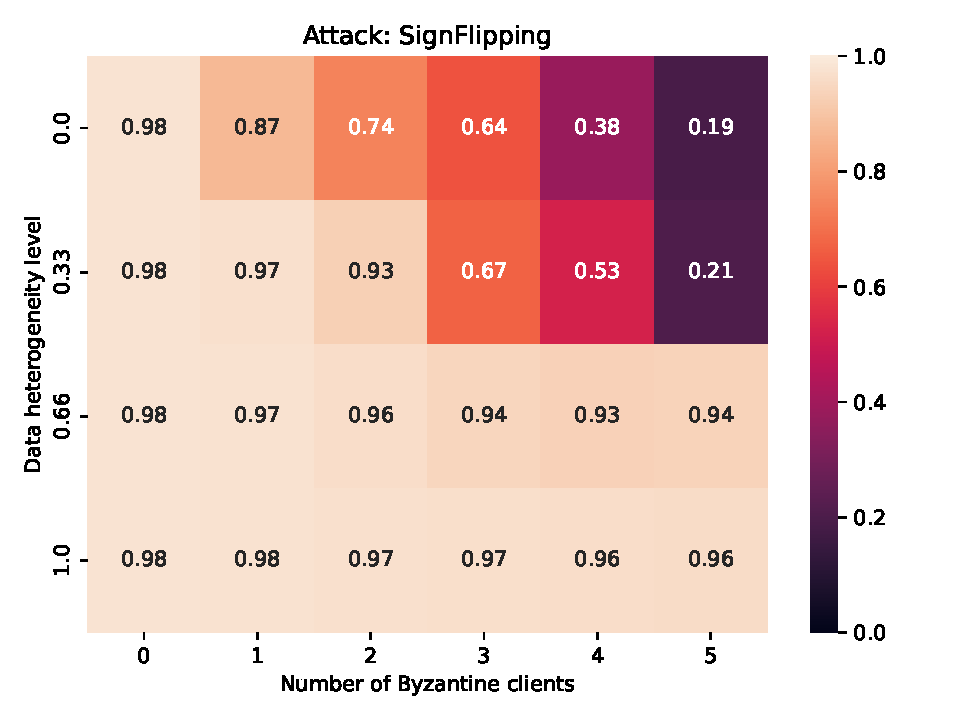
\includegraphics[width=\textwidth]{../plots/cnn_tanh_heatmaps/test_SignFlipping_mnist_cnn_mnist_tanh_gamma_similarity_niid_NNM_ARC_GeometricMedian_nb_honest_clients_10_tolerated_f_equal_real.pdf}
        \caption{CNN Tanh}
        \label{fig:gm_sf_tanh}
    \end{subfigure}
    \hfill
    \begin{subfigure}[b]{0.24\textwidth}
        \centering
        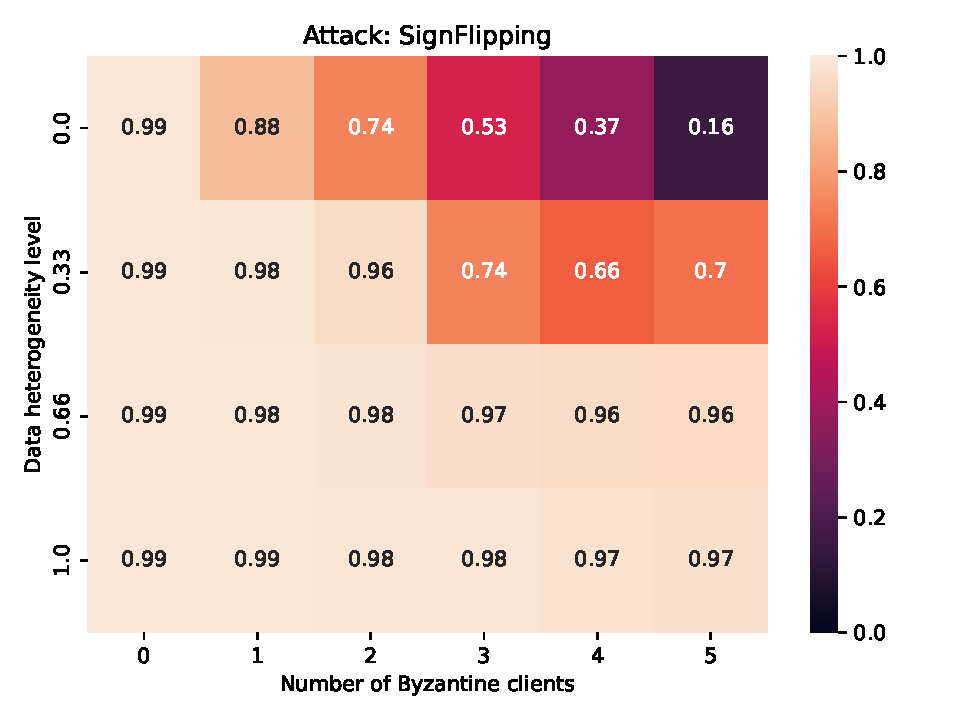
\includegraphics[width=\textwidth]{../plots/cnn_clipped_heatmaps/test_SignFlipping_mnist_cnn_mnist_gamma_similarity_niid_NNM_ARC_GeometricMedian_nb_honest_clients_10_tolerated_f_equal_real.pdf}
        \caption{CNN ReLU (Grad-Norm Clip $=21$)}
        \label{fig:gm_sf_gradclip21}
    \end{subfigure}
    \caption{Geometric Median (GM) under Sign Flipping Attack.}
    \label{fig:gm_sf_grid}
\end{figure}
\clearpage
\subsubsection{GM under IPM}
\begin{figure}[htbp]
    \centering
    \begin{subfigure}[b]{0.24\textwidth}
        \centering
        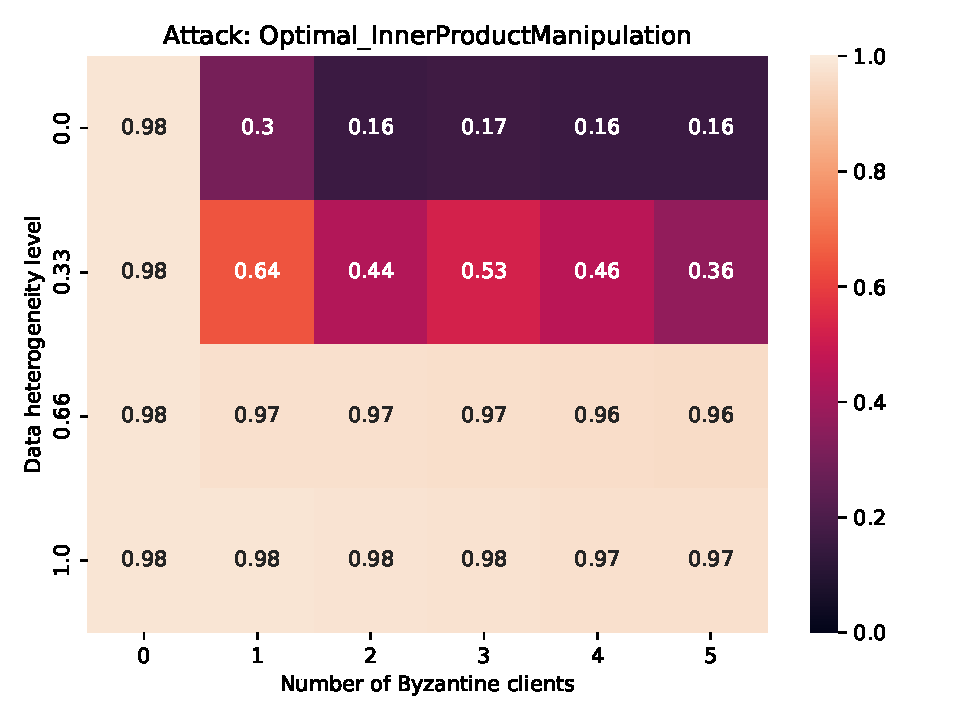
\includegraphics[width=\textwidth]{../plots/mnist_clipping_heatmaps/cnn_mnist/test_Optimal_InnerProductManipulation_mnist_cnn_mnist_gamma_similarity_niid_NNM_ARC_GeometricMedian_nb_honest_clients_10_tolerated_f_equal_real.pdf}
        \caption{CNN ReLU (No Clip)}
        \label{fig:gm_ipm_noclip}
    \end{subfigure}
    \hfill
    \begin{subfigure}[b]{0.24\textwidth}
        \centering
        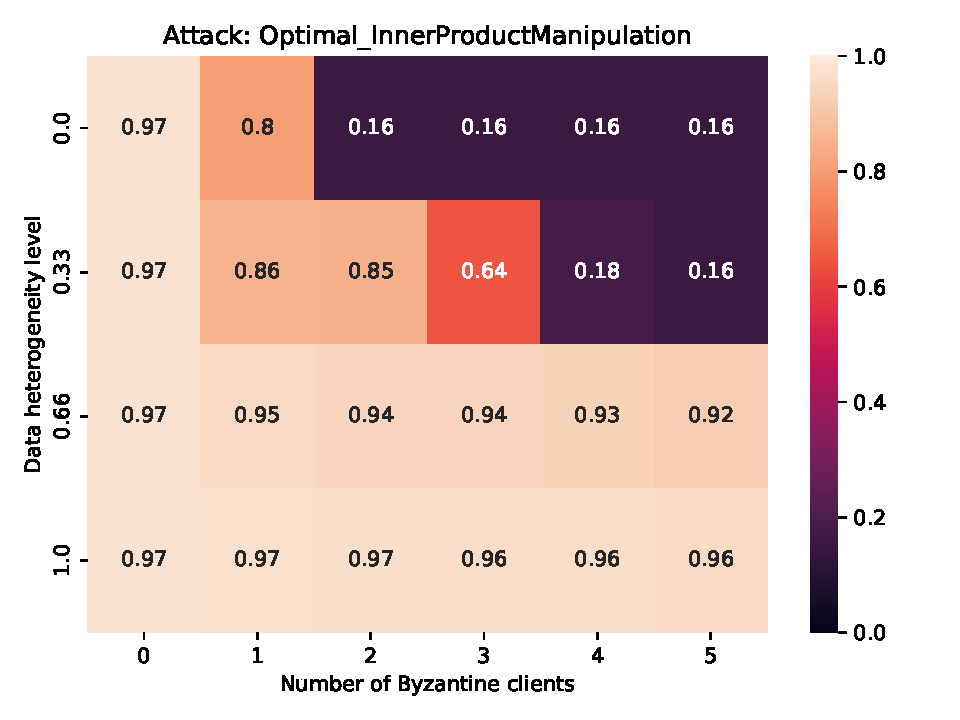
\includegraphics[width=\textwidth]{../plots/mnist_clipping_heatmaps/cnn_mnist_clipping_1/test_Optimal_InnerProductManipulation_mnist_cnn_mnist_clipping_1_gamma_similarity_niid_NNM_ARC_GeometricMedian_nb_honest_clients_10_tolerated_f_equal_real.pdf}
        \caption{CNN ReLU (Clip $=1$)}
        \label{fig:gm_ipm_clip1}
    \end{subfigure}
    \hfill
    \begin{subfigure}[b]{0.24\textwidth}
        \centering
        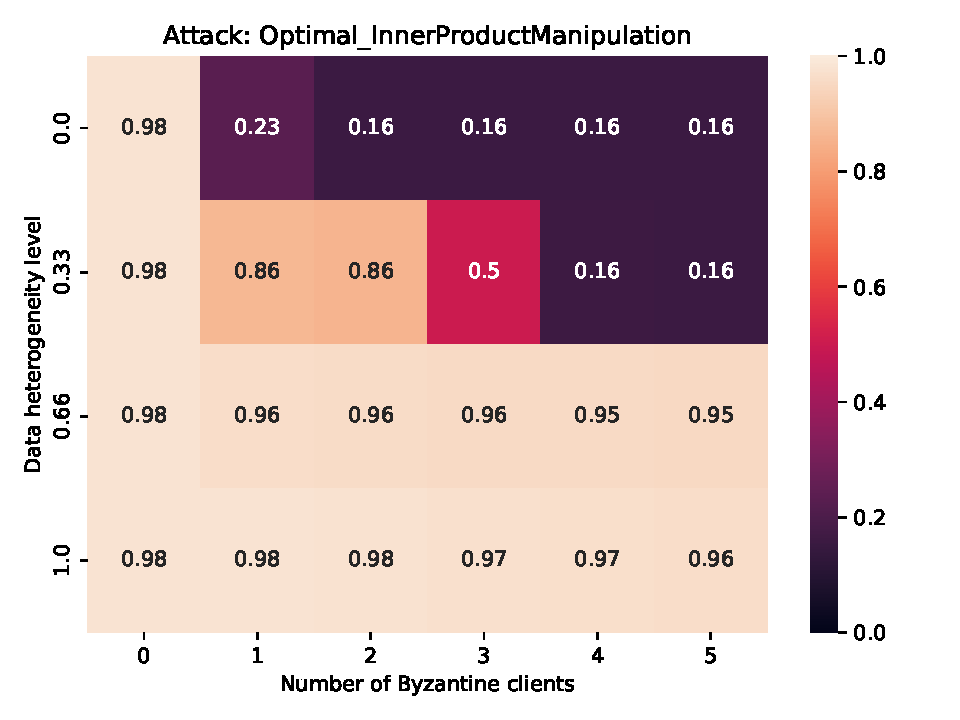
\includegraphics[width=\textwidth]{../plots/mnist_clipping_heatmaps/cnn_mnist_clipping_2/test_Optimal_InnerProductManipulation_mnist_cnn_mnist_clipping_2_gamma_similarity_niid_NNM_ARC_GeometricMedian_nb_honest_clients_10_tolerated_f_equal_real.pdf}
        \caption{CNN ReLU (Clip $=2$)}
        \label{fig:gm_ipm_clip2}
    \end{subfigure}
    \vspace{0.3cm}
    \begin{subfigure}[b]{0.24\textwidth}
        \centering
        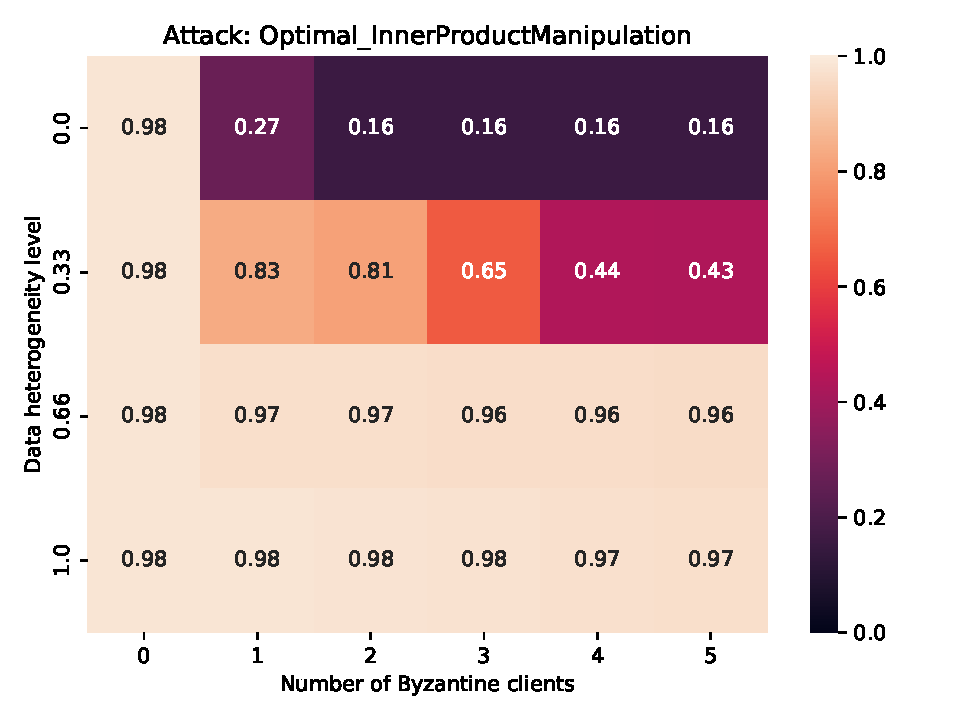
\includegraphics[width=\textwidth]{../plots/mnist_clipping_heatmaps/cnn_mnist_clipping_4/test_Optimal_InnerProductManipulation_mnist_cnn_mnist_clipping_4_gamma_similarity_niid_NNM_ARC_GeometricMedian_nb_honest_clients_10_tolerated_f_equal_real.pdf}
        \caption{CNN ReLU (Clip $=4$)}
        \label{fig:gm_ipm_clip4}
    \end{subfigure}
    \hfill
    \begin{subfigure}[b]{0.24\textwidth}
        \centering
        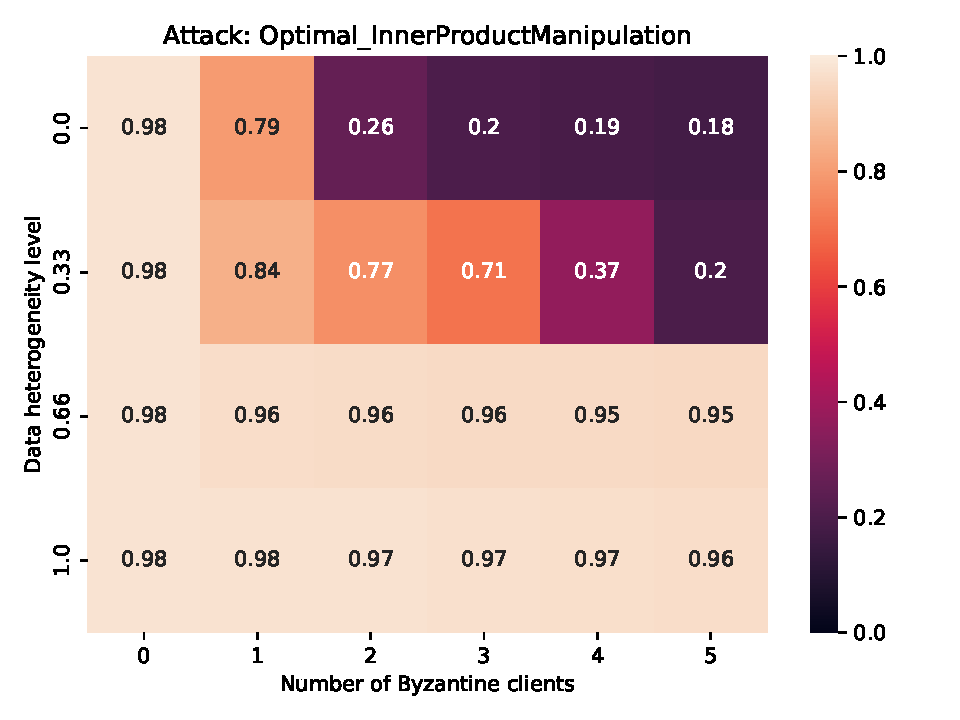
\includegraphics[width=\textwidth]{../plots/cnn_tanh_heatmaps/test_Optimal_InnerProductManipulation_mnist_cnn_mnist_tanh_gamma_similarity_niid_NNM_ARC_GeometricMedian_nb_honest_clients_10_tolerated_f_equal_real.pdf}
        \caption{CNN Tanh}
        \label{fig:gm_ipm_tanh}
    \end{subfigure}
    \hfill
    \begin{subfigure}[b]{0.24\textwidth}
        \centering
        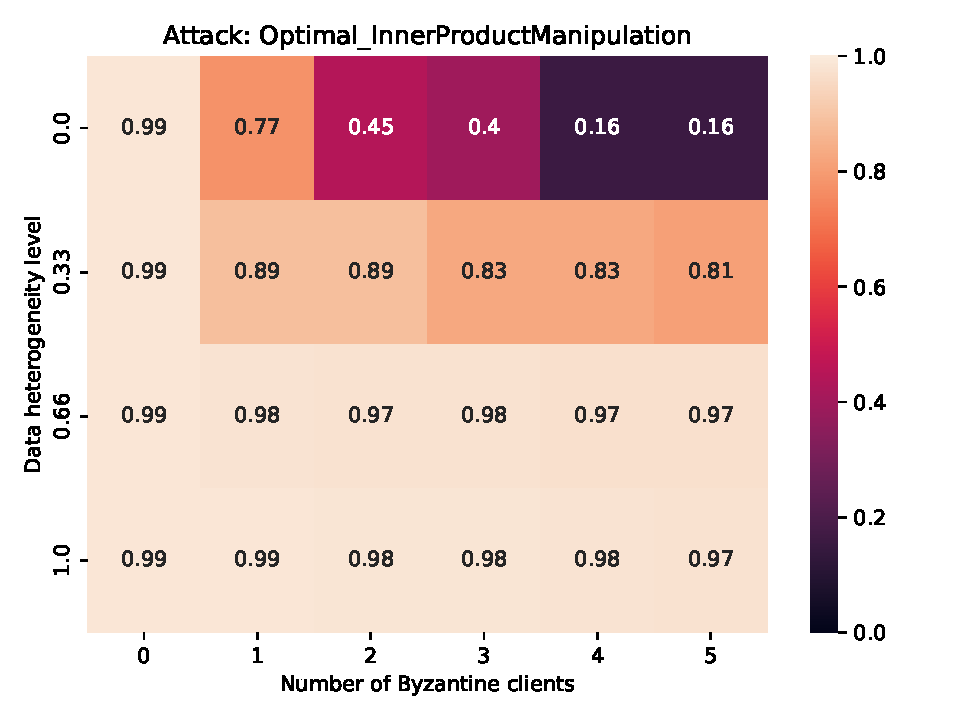
\includegraphics[width=\textwidth]{../plots/cnn_clipped_heatmaps/test_Optimal_InnerProductManipulation_mnist_cnn_mnist_gamma_similarity_niid_NNM_ARC_GeometricMedian_nb_honest_clients_10_tolerated_f_equal_real.pdf}
        \caption{CNN ReLU (Grad-Norm Clip $=21$)}
        \label{fig:gm_ipm_gradclip21}
    \end{subfigure}
    \caption{Geometric Median (GM) under Optimal IPM Attack.}
    \label{fig:gm_ipm_grid}
\end{figure}
\clearpage
\subsection{Multi-Krum (MK)}
\subsubsection{MK under Worst-Case across all Attacks}
\begin{figure}[htbp]
    \centering
    \begin{subfigure}[b]{0.24\textwidth}
        \centering
        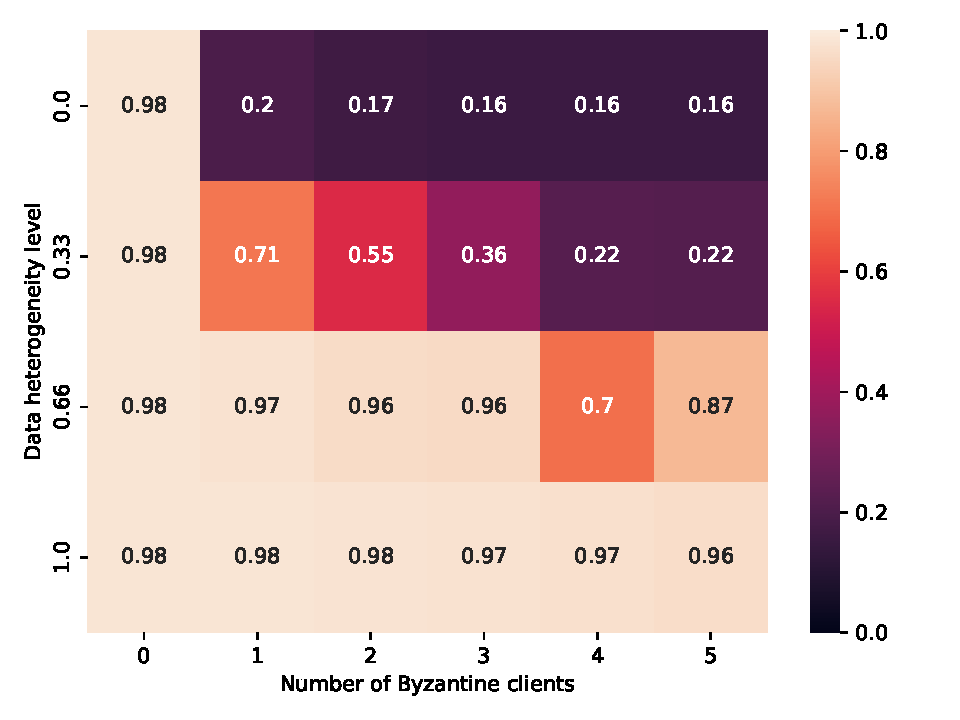
\includegraphics[width=\textwidth]{../plots/mnist_clipping_heatmaps/cnn_mnist/test_mnist_cnn_mnist_gamma_similarity_niid_NNM_ARC_MultiKrum_nb_honest_clients_10_tolerated_f_equal_real.pdf}
        \caption{CNN ReLU (No Clip)}
        \label{fig:mk_worst_case_noclip}
    \end{subfigure}
    \hfill
    \begin{subfigure}[b]{0.24\textwidth}
        \centering
        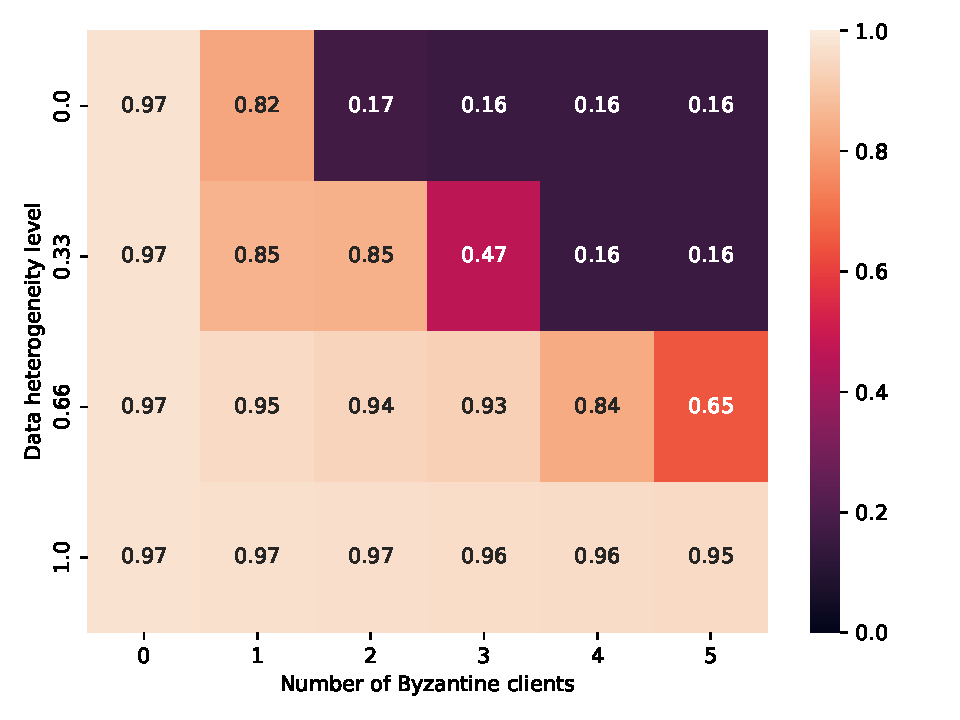
\includegraphics[width=\textwidth]{../plots/mnist_clipping_heatmaps/cnn_mnist_clipping_1/test_mnist_cnn_mnist_clipping_1_gamma_similarity_niid_NNM_ARC_MultiKrum_nb_honest_clients_10_tolerated_f_equal_real.pdf}
        \caption{CNN ReLU (Clip $=1$)}
        \label{fig:mk_worst_case_clip1}
    \end{subfigure}
    \hfill
    \begin{subfigure}[b]{0.24\textwidth}
        \centering
        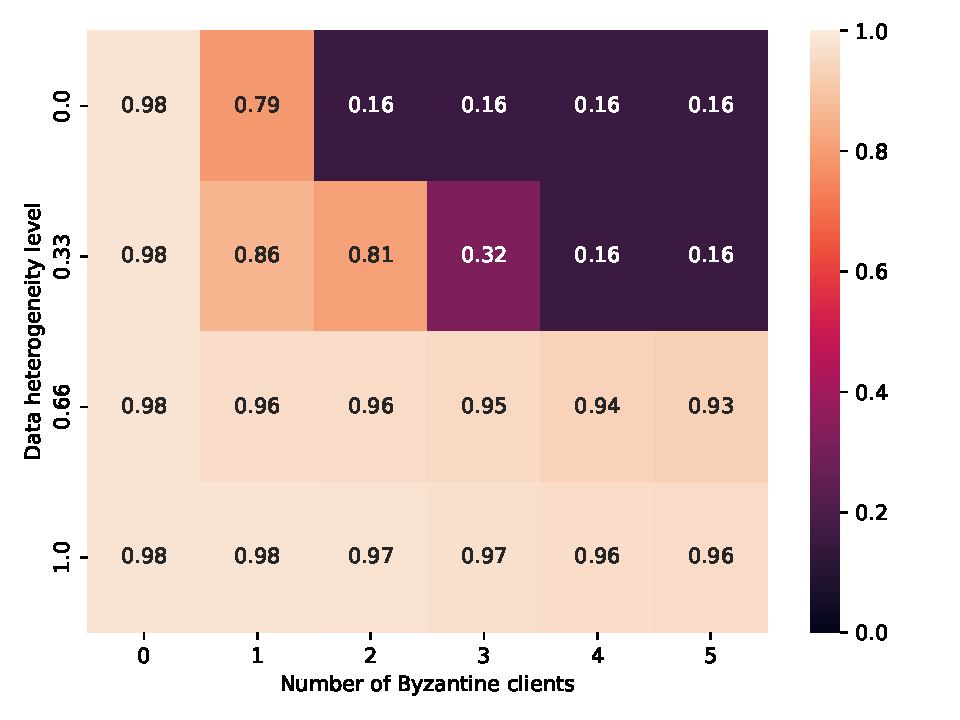
\includegraphics[width=\textwidth]{../plots/mnist_clipping_heatmaps/cnn_mnist_clipping_2/test_mnist_cnn_mnist_clipping_2_gamma_similarity_niid_NNM_ARC_MultiKrum_nb_honest_clients_10_tolerated_f_equal_real.pdf}
        \caption{CNN ReLU (Clip $=2$)}
        \label{fig:mk_worst_case_clip2}
    \end{subfigure}
    \vspace{0.3cm}
    \begin{subfigure}[b]{0.24\textwidth}
        \centering
        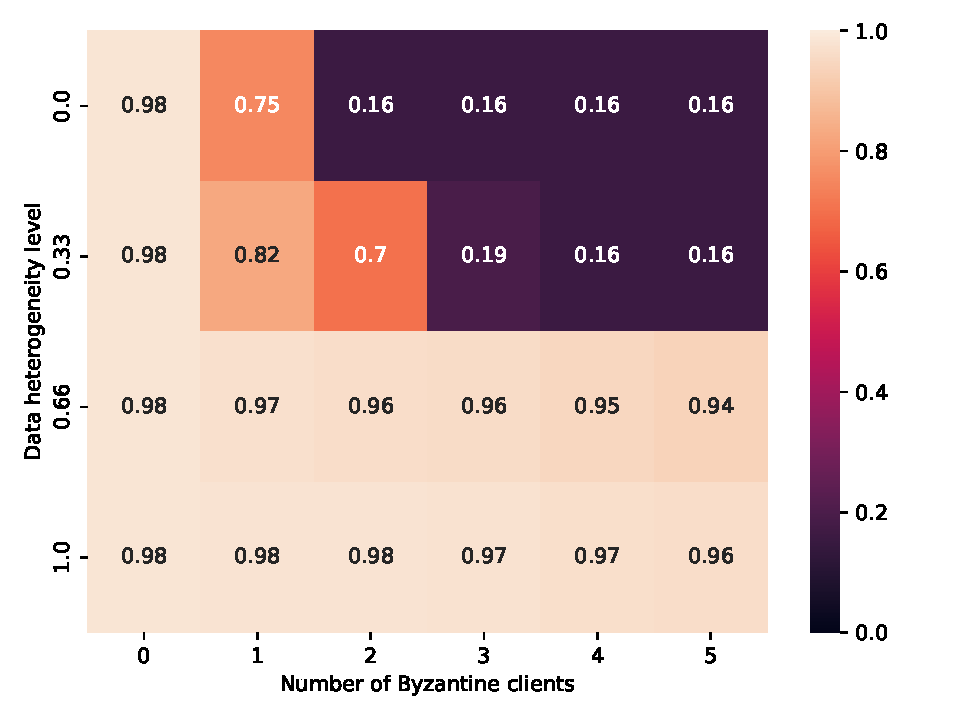
\includegraphics[width=\textwidth]{../plots/mnist_clipping_heatmaps/cnn_mnist_clipping_4/test_mnist_cnn_mnist_clipping_4_gamma_similarity_niid_NNM_ARC_MultiKrum_nb_honest_clients_10_tolerated_f_equal_real.pdf}
        \caption{CNN ReLU (Clip $=4$)}
        \label{fig:mk_worst_case_clip4}
    \end{subfigure}
    \hfill
    \begin{subfigure}[b]{0.24\textwidth}
        \centering
        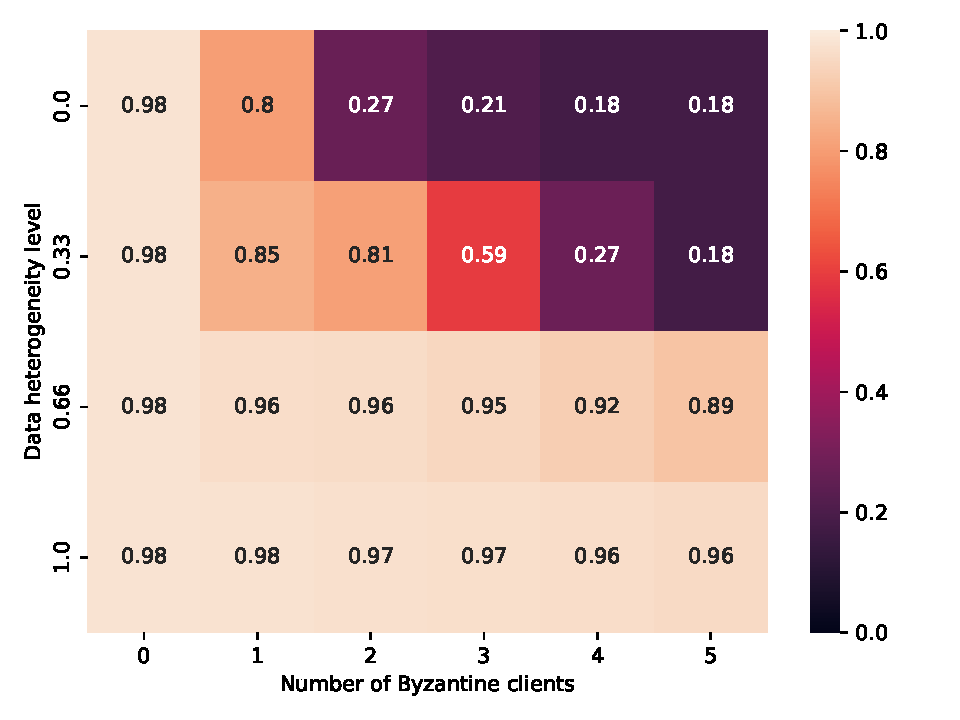
\includegraphics[width=\textwidth]{../plots/cnn_tanh_heatmaps/test_mnist_cnn_mnist_tanh_gamma_similarity_niid_NNM_ARC_MultiKrum_nb_honest_clients_10_tolerated_f_equal_real.pdf}
        \caption{CNN Tanh}
        \label{fig:mk_worst_case_tanh}
    \end{subfigure}
    \caption{Multi-Krum (MK) under Worst-Case across all Attacks.}
    \label{fig:mk_worst_case_grid}
\end{figure}
\clearpage
\subsubsection{MK under ALIE}
\begin{figure}[htbp]
    \centering
    \begin{subfigure}[b]{0.24\textwidth}
        \centering
        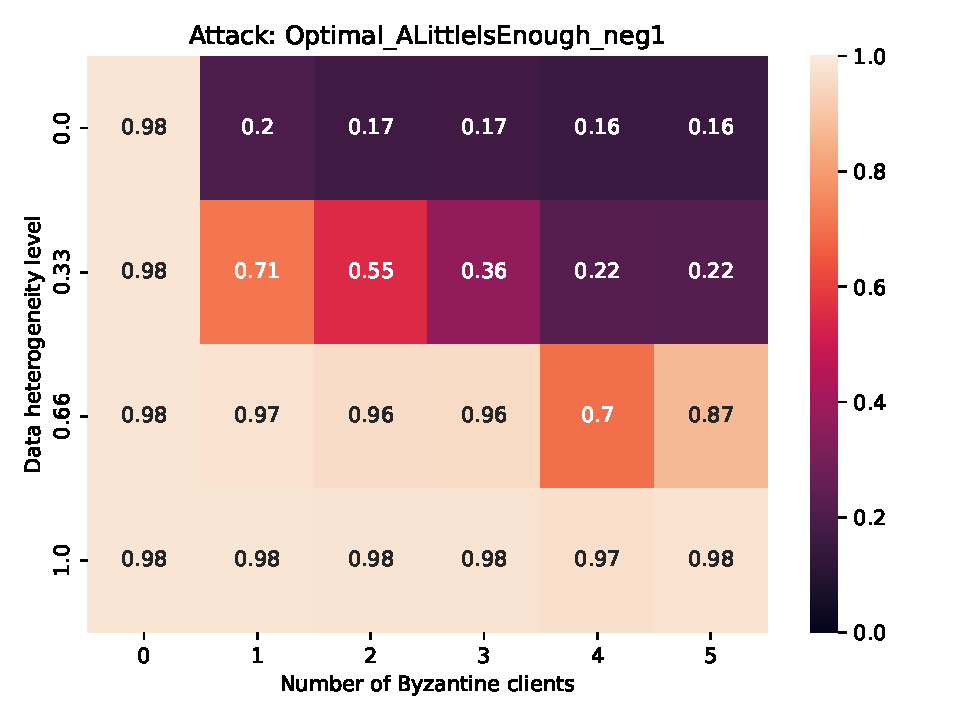
\includegraphics[width=\textwidth]{../plots/mnist_clipping_heatmaps/cnn_mnist/test_Optimal_ALittleIsEnough_neg1_mnist_cnn_mnist_gamma_similarity_niid_NNM_ARC_MultiKrum_nb_honest_clients_10_tolerated_f_equal_real.pdf}
        \caption{CNN ReLU (No Clip)}
        \label{fig:mk_alie_noclip}
    \end{subfigure}
    \hfill
    \begin{subfigure}[b]{0.24\textwidth}
        \centering
        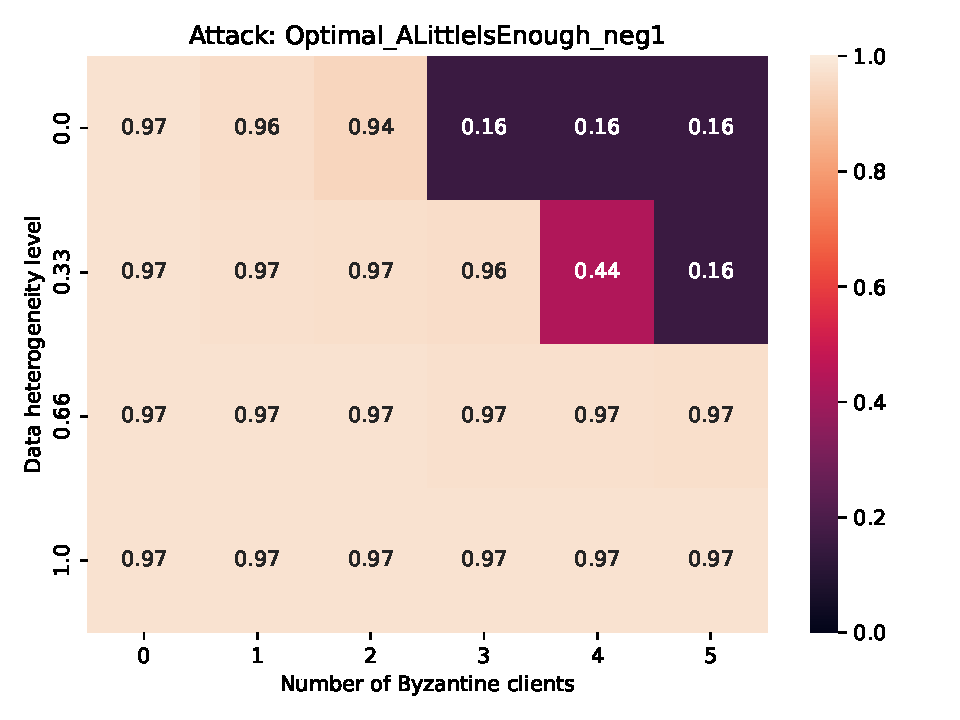
\includegraphics[width=\textwidth]{../plots/mnist_clipping_heatmaps/cnn_mnist_clipping_1/test_Optimal_ALittleIsEnough_neg1_mnist_cnn_mnist_clipping_1_gamma_similarity_niid_NNM_ARC_MultiKrum_nb_honest_clients_10_tolerated_f_equal_real.pdf}
        \caption{CNN ReLU (Clip $=1$)}
        \label{fig:mk_alie_clip1}
    \end{subfigure}
    \hfill
    \begin{subfigure}[b]{0.24\textwidth}
        \centering
        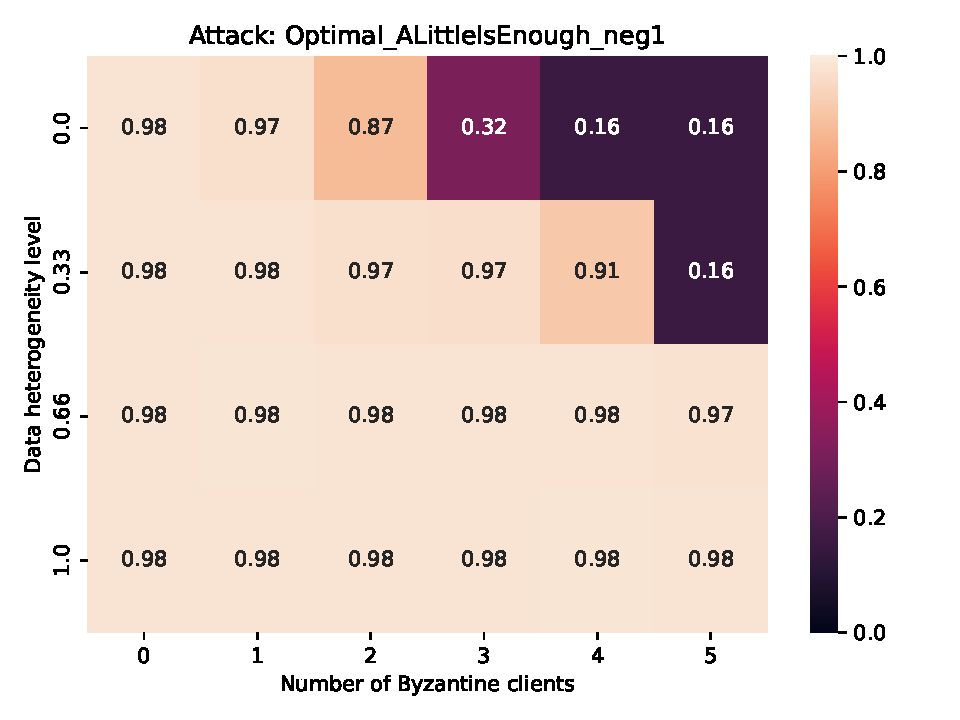
\includegraphics[width=\textwidth]{../plots/mnist_clipping_heatmaps/cnn_mnist_clipping_2/test_Optimal_ALittleIsEnough_neg1_mnist_cnn_mnist_clipping_2_gamma_similarity_niid_NNM_ARC_MultiKrum_nb_honest_clients_10_tolerated_f_equal_real.pdf}
        \caption{CNN ReLU (Clip $=2$)}
        \label{fig:mk_alie_clip2}
    \end{subfigure}
    \vspace{0.3cm}
    \begin{subfigure}[b]{0.24\textwidth}
        \centering
        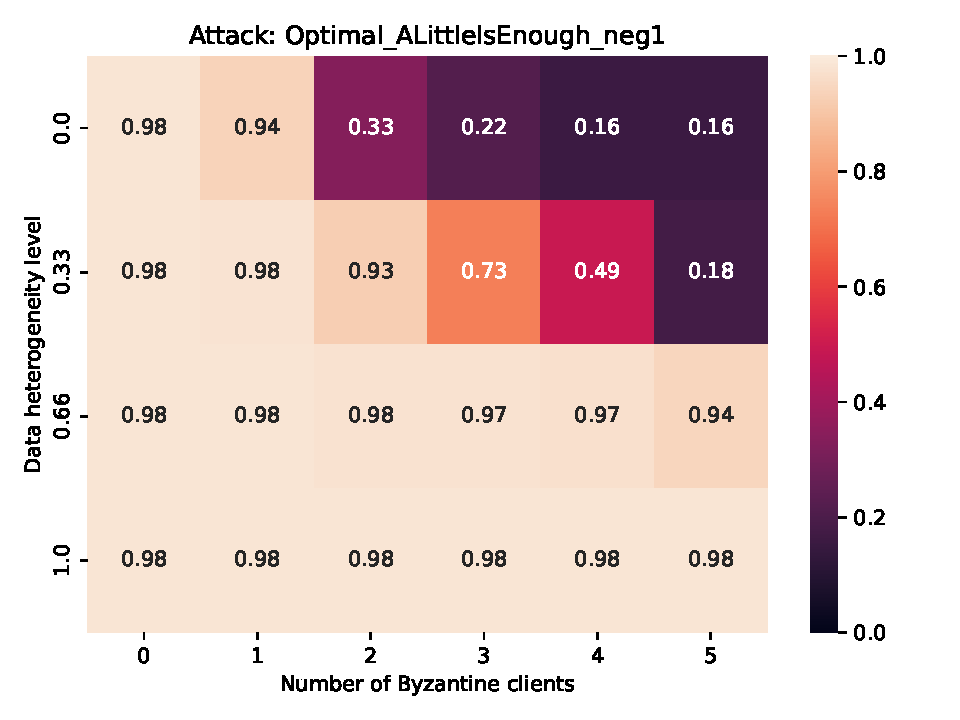
\includegraphics[width=\textwidth]{../plots/mnist_clipping_heatmaps/cnn_mnist_clipping_4/test_Optimal_ALittleIsEnough_neg1_mnist_cnn_mnist_clipping_4_gamma_similarity_niid_NNM_ARC_MultiKrum_nb_honest_clients_10_tolerated_f_equal_real.pdf}
        \caption{CNN ReLU (Clip $=4$)}
        \label{fig:mk_alie_clip4}
    \end{subfigure}
    \hfill
    \begin{subfigure}[b]{0.24\textwidth}
        \centering
        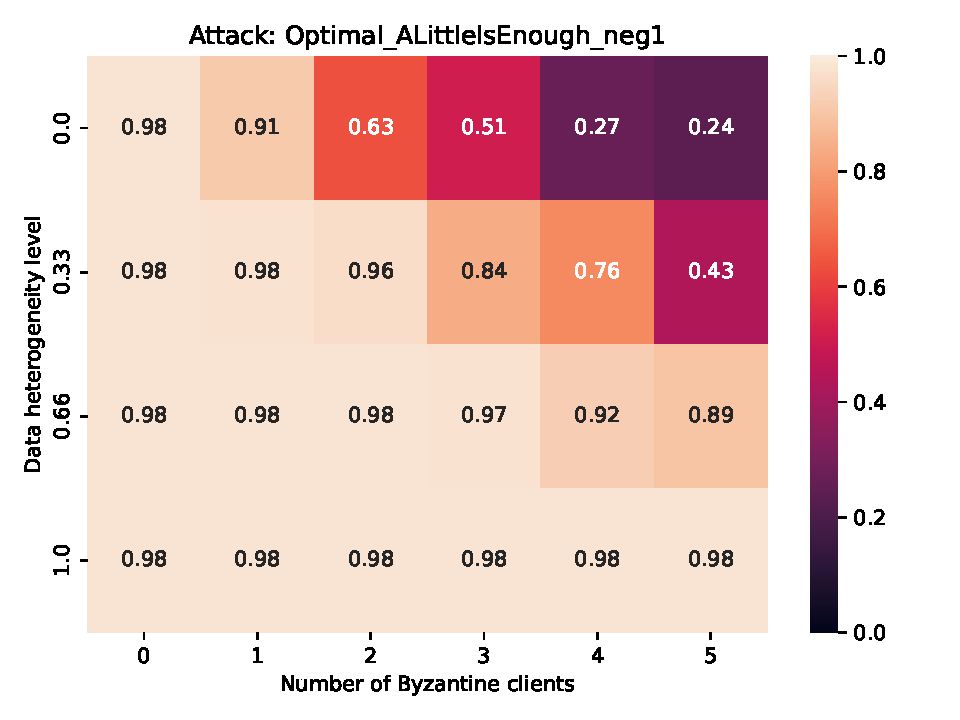
\includegraphics[width=\textwidth]{../plots/cnn_tanh_heatmaps/test_Optimal_ALittleIsEnough_neg1_mnist_cnn_mnist_tanh_gamma_similarity_niid_NNM_ARC_MultiKrum_nb_honest_clients_10_tolerated_f_equal_real.pdf}
        \caption{CNN Tanh}
        \label{fig:mk_alie_tanh}
    \end{subfigure}
    \caption{Multi-Krum (MK) under Optimal ALIE Attack.}
    \label{fig:mk_alie_grid}
\end{figure}
\clearpage
\subsubsection{MK under SF}
\begin{figure}[htbp]
    \centering
    \begin{subfigure}[b]{0.24\textwidth}
        \centering
        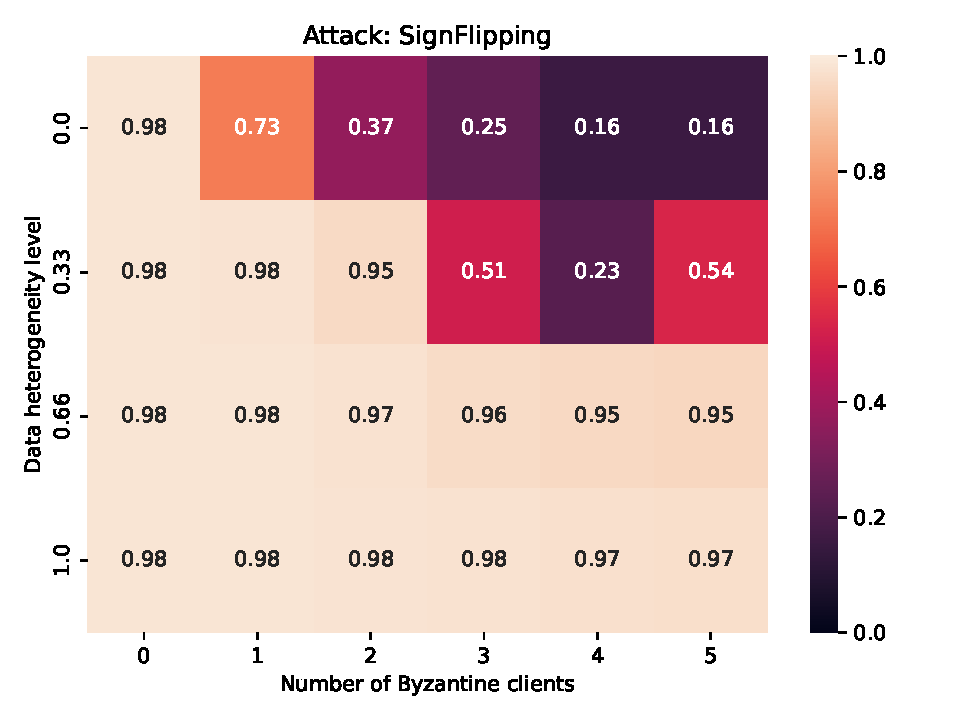
\includegraphics[width=\textwidth]{../plots/mnist_clipping_heatmaps/cnn_mnist/test_SignFlipping_mnist_cnn_mnist_gamma_similarity_niid_NNM_ARC_MultiKrum_nb_honest_clients_10_tolerated_f_equal_real.pdf}
        \caption{CNN ReLU (No Clip)}
        \label{fig:mk_sf_noclip}
    \end{subfigure}
    \hfill
    \begin{subfigure}[b]{0.24\textwidth}
        \centering
        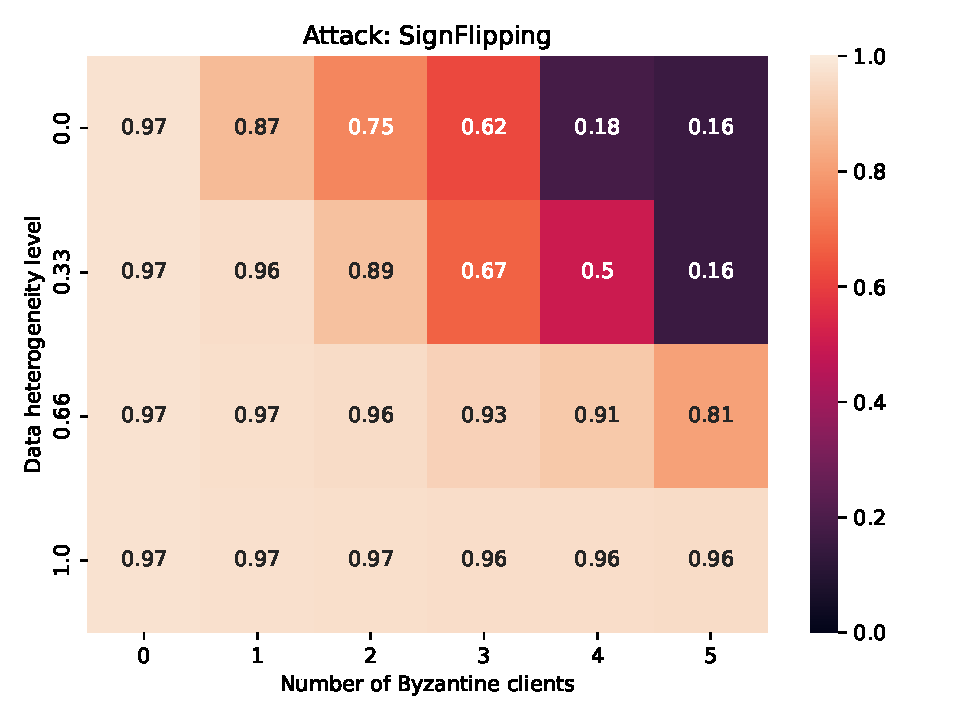
\includegraphics[width=\textwidth]{../plots/mnist_clipping_heatmaps/cnn_mnist_clipping_1/test_SignFlipping_mnist_cnn_mnist_clipping_1_gamma_similarity_niid_NNM_ARC_MultiKrum_nb_honest_clients_10_tolerated_f_equal_real.pdf}
        \caption{CNN ReLU (Clip $=1$)}
        \label{fig:mk_sf_clip1}
    \end{subfigure}
    \hfill
    \begin{subfigure}[b]{0.24\textwidth}
        \centering
        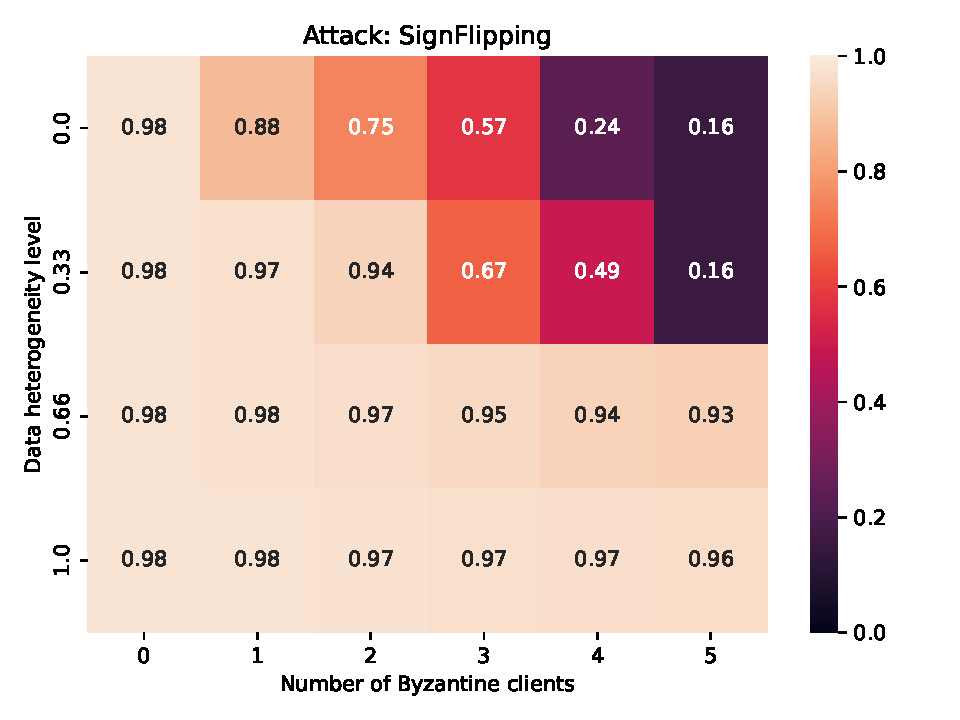
\includegraphics[width=\textwidth]{../plots/mnist_clipping_heatmaps/cnn_mnist_clipping_2/test_SignFlipping_mnist_cnn_mnist_clipping_2_gamma_similarity_niid_NNM_ARC_MultiKrum_nb_honest_clients_10_tolerated_f_equal_real.pdf}
        \caption{CNN ReLU (Clip $=2$)}
        \label{fig:mk_sf_clip2}
    \end{subfigure}
    \vspace{0.3cm}
    \begin{subfigure}[b]{0.24\textwidth}
        \centering
        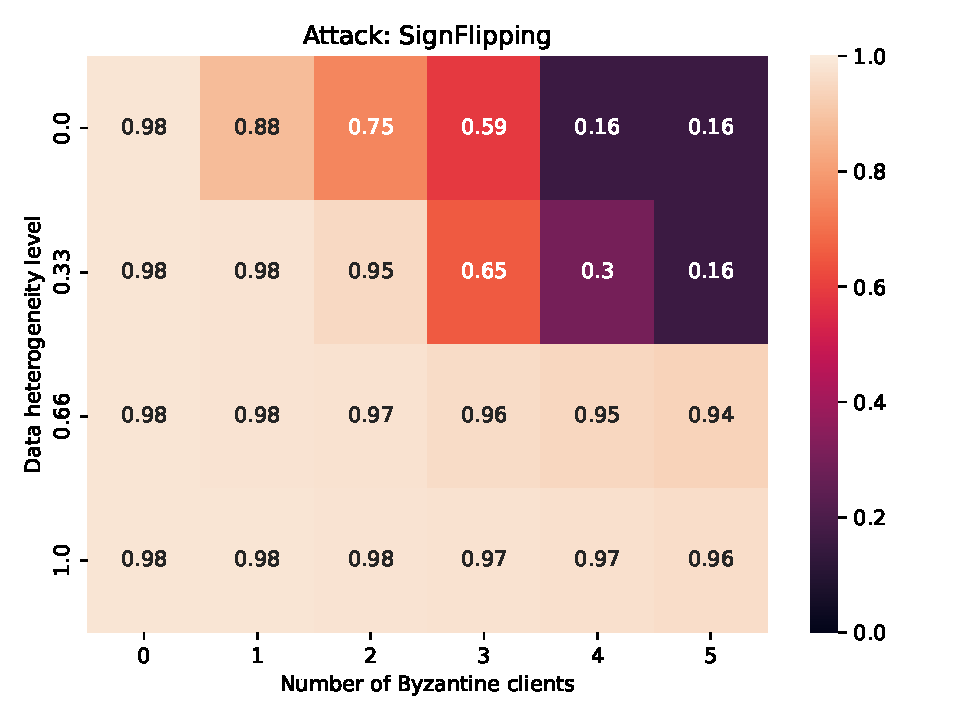
\includegraphics[width=\textwidth]{../plots/mnist_clipping_heatmaps/cnn_mnist_clipping_4/test_SignFlipping_mnist_cnn_mnist_clipping_4_gamma_similarity_niid_NNM_ARC_MultiKrum_nb_honest_clients_10_tolerated_f_equal_real.pdf}
        \caption{CNN ReLU (Clip $=4$)}
        \label{fig:mk_sf_clip4}
    \end{subfigure}
    \hfill
    \begin{subfigure}[b]{0.24\textwidth}
        \centering
        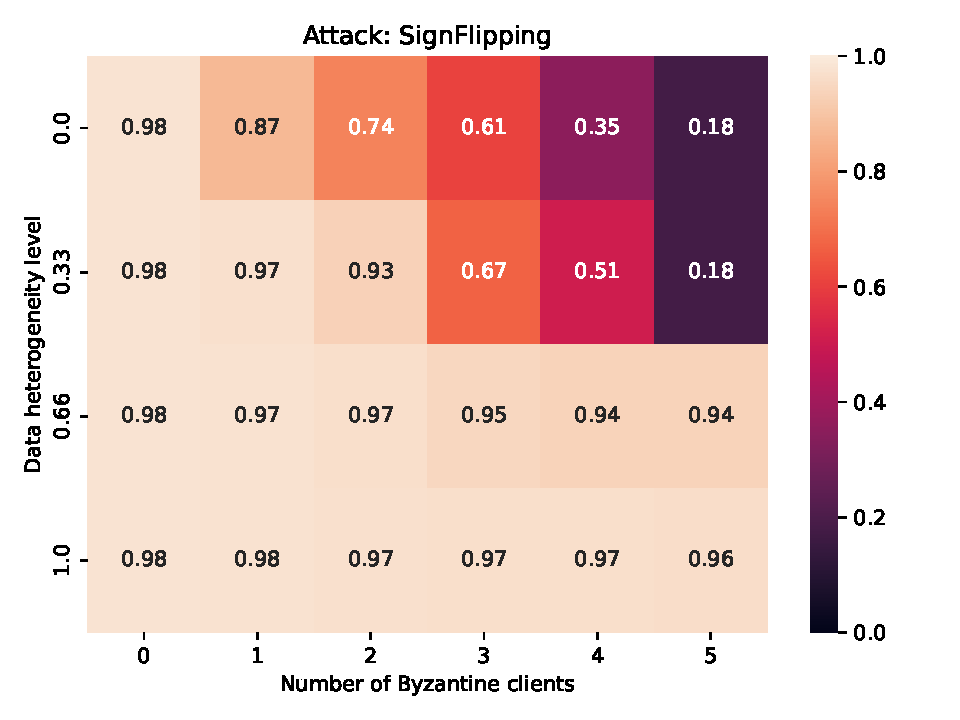
\includegraphics[width=\textwidth]{../plots/cnn_tanh_heatmaps/test_SignFlipping_mnist_cnn_mnist_tanh_gamma_similarity_niid_NNM_ARC_MultiKrum_nb_honest_clients_10_tolerated_f_equal_real.pdf}
        \caption{CNN Tanh}
        \label{fig:mk_sf_tanh}
    \end{subfigure}
    \caption{Multi-Krum (MK) under Sign Flipping Attack.}
    \label{fig:mk_sf_grid}
\end{figure}
\clearpage
\subsubsection{MK under IPM}
\begin{figure}[htbp]
    \centering
    \begin{subfigure}[b]{0.24\textwidth}
        \centering
        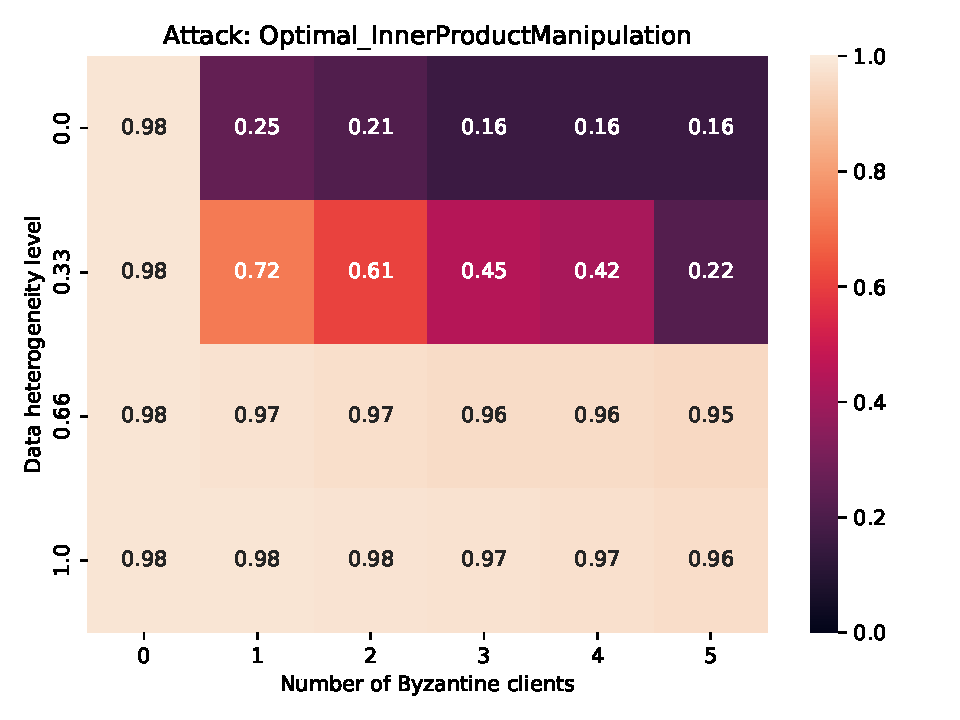
\includegraphics[width=\textwidth]{../plots/mnist_clipping_heatmaps/cnn_mnist/test_Optimal_InnerProductManipulation_mnist_cnn_mnist_gamma_similarity_niid_NNM_ARC_MultiKrum_nb_honest_clients_10_tolerated_f_equal_real.pdf}
        \caption{CNN ReLU (No Clip)}
        \label{fig:mk_ipm_noclip}
    \end{subfigure}
    \hfill
    \begin{subfigure}[b]{0.24\textwidth}
        \centering
        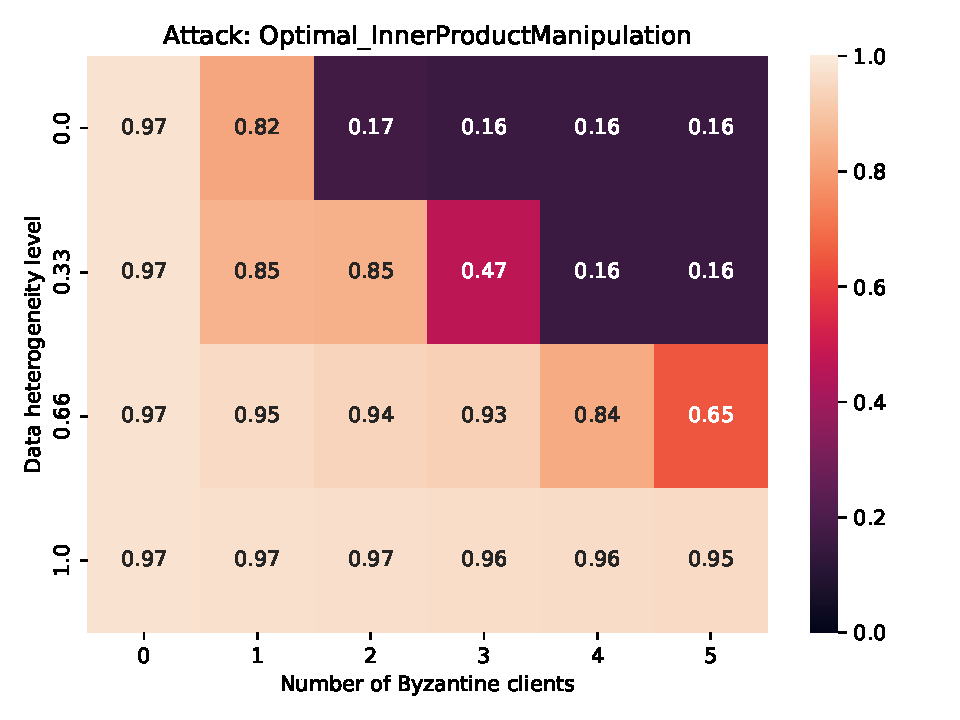
\includegraphics[width=\textwidth]{../plots/mnist_clipping_heatmaps/cnn_mnist_clipping_1/test_Optimal_InnerProductManipulation_mnist_cnn_mnist_clipping_1_gamma_similarity_niid_NNM_ARC_MultiKrum_nb_honest_clients_10_tolerated_f_equal_real.pdf}
        \caption{CNN ReLU (Clip $=1$)}
        \label{fig:mk_ipm_clip1}
    \end{subfigure}
    \hfill
    \begin{subfigure}[b]{0.24\textwidth}
        \centering
        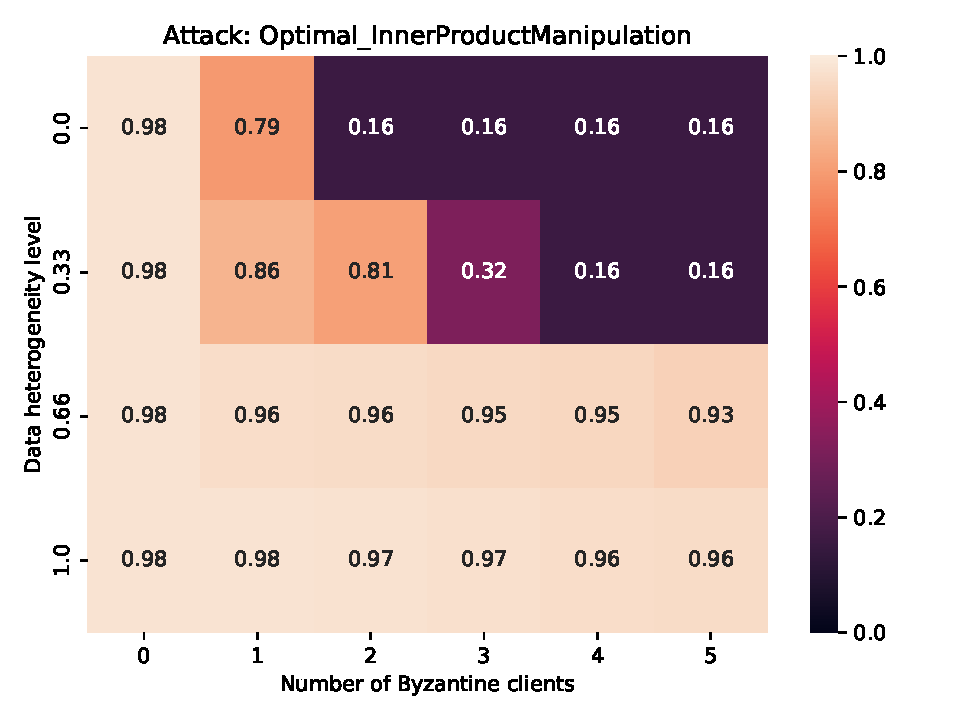
\includegraphics[width=\textwidth]{../plots/mnist_clipping_heatmaps/cnn_mnist_clipping_2/test_Optimal_InnerProductManipulation_mnist_cnn_mnist_clipping_2_gamma_similarity_niid_NNM_ARC_MultiKrum_nb_honest_clients_10_tolerated_f_equal_real.pdf}
        \caption{CNN ReLU (Clip $=2$)}
        \label{fig:mk_ipm_clip2}
    \end{subfigure}
    \vspace{0.3cm}
    \begin{subfigure}[b]{0.24\textwidth}
        \centering
        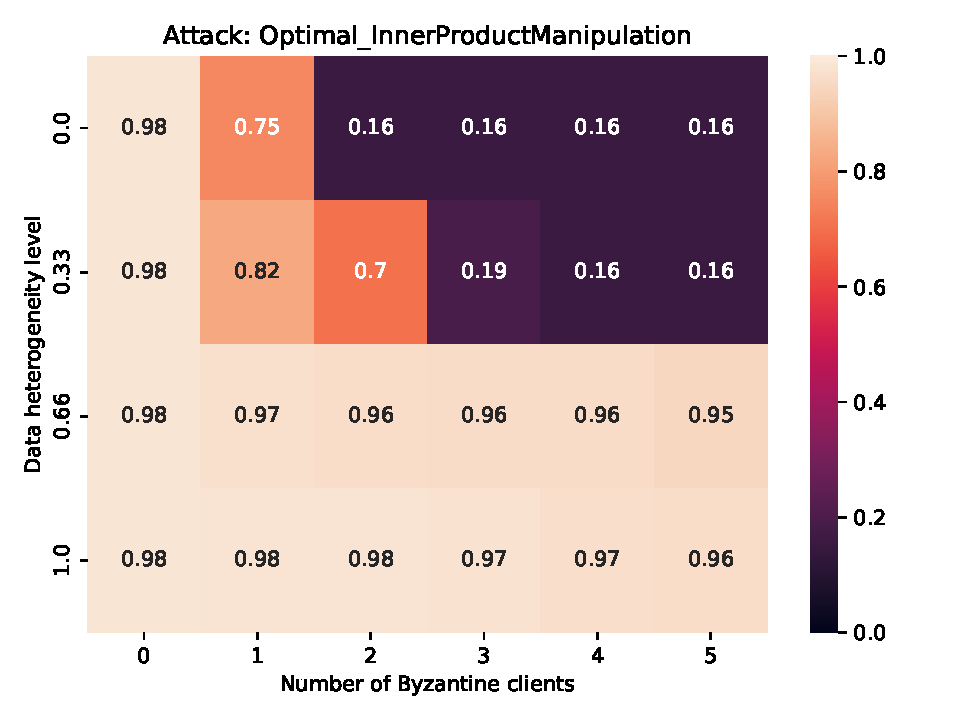
\includegraphics[width=\textwidth]{../plots/mnist_clipping_heatmaps/cnn_mnist_clipping_4/test_Optimal_InnerProductManipulation_mnist_cnn_mnist_clipping_4_gamma_similarity_niid_NNM_ARC_MultiKrum_nb_honest_clients_10_tolerated_f_equal_real.pdf}
        \caption{CNN ReLU (Clip $=4$)}
        \label{fig:mk_ipm_clip4}
    \end{subfigure}
    \hfill
    \begin{subfigure}[b]{0.24\textwidth}
        \centering
        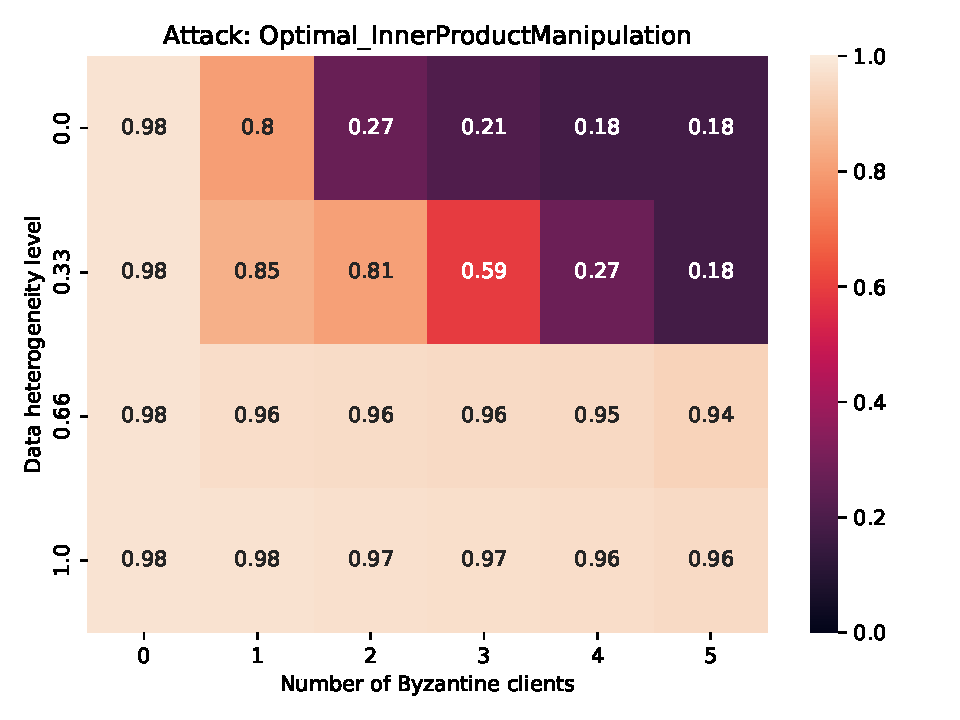
\includegraphics[width=\textwidth]{../plots/cnn_tanh_heatmaps/test_Optimal_InnerProductManipulation_mnist_cnn_mnist_tanh_gamma_similarity_niid_NNM_ARC_MultiKrum_nb_honest_clients_10_tolerated_f_equal_real.pdf}
        \caption{CNN Tanh}
        \label{fig:mk_ipm_tanh}
    \end{subfigure}
    \caption{Multi-Krum (MK) under Optimal IPM Attack.}
    \label{fig:mk_ipm_grid}
\end{figure}
\clearpage
\subsection{Trimmed Mean (TM)}
\subsubsection{TM under Worst-Case across all Attacks}
\begin{figure}[htbp]
    \centering
    \begin{subfigure}[b]{0.24\textwidth}
        \centering
        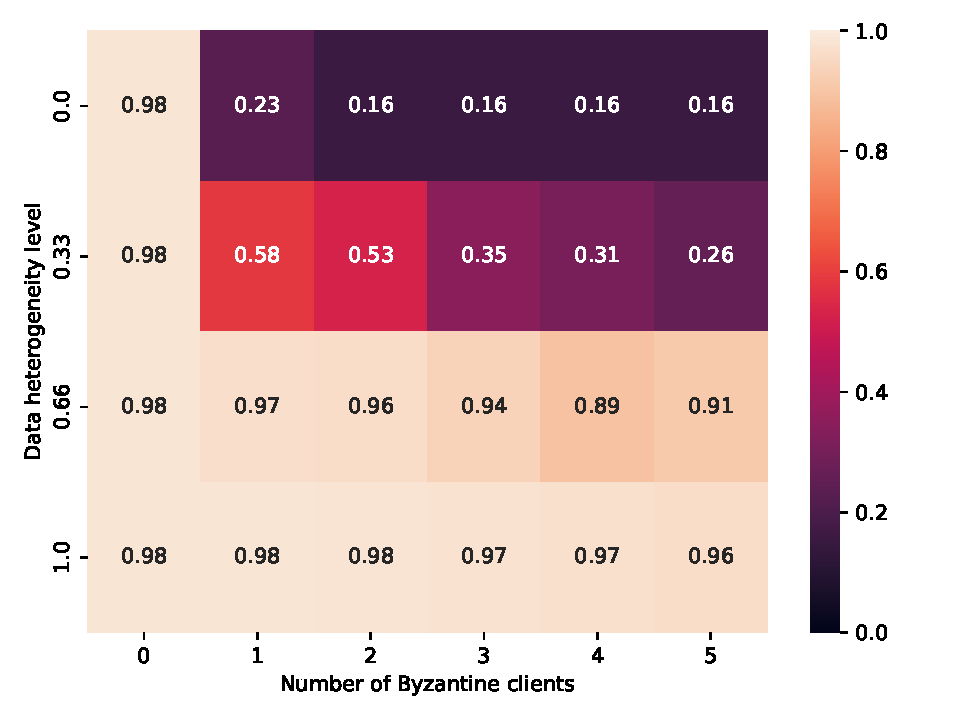
\includegraphics[width=\textwidth]{../plots/mnist_clipping_heatmaps/cnn_mnist/test_mnist_cnn_mnist_gamma_similarity_niid_NNM_ARC_TrMean_nb_honest_clients_10_tolerated_f_equal_real.pdf}
        \caption{CNN ReLU (No Clip)}
        \label{fig:tm_worst_case_noclip}
    \end{subfigure}
    \hfill
    \begin{subfigure}[b]{0.24\textwidth}
        \centering
        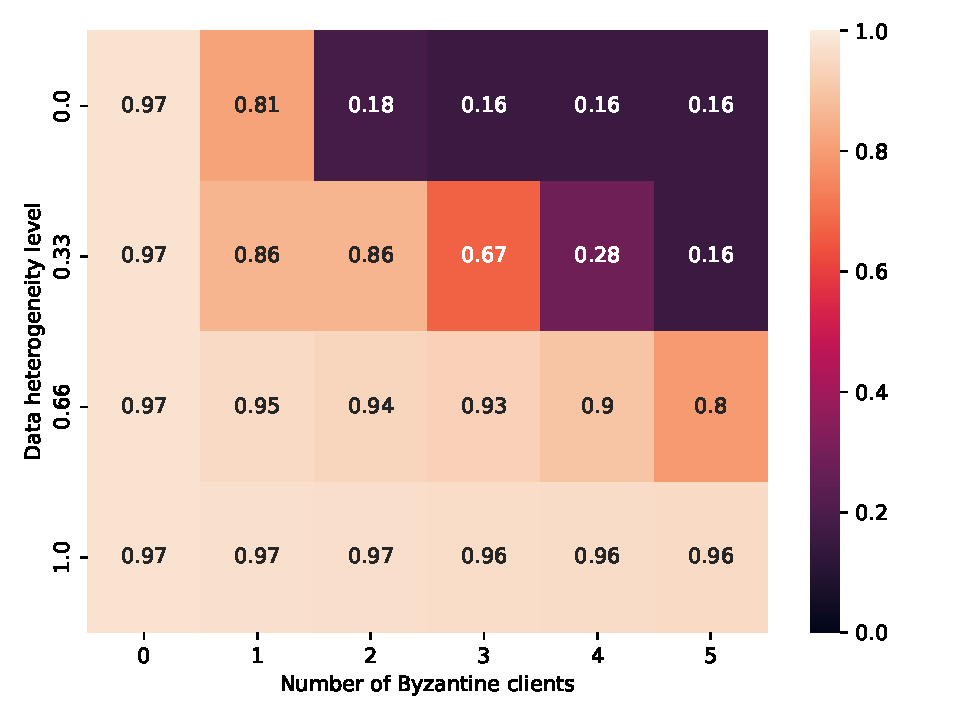
\includegraphics[width=\textwidth]{../plots/mnist_clipping_heatmaps/cnn_mnist_clipping_1/test_mnist_cnn_mnist_clipping_1_gamma_similarity_niid_NNM_ARC_TrMean_nb_honest_clients_10_tolerated_f_equal_real.pdf}
        \caption{CNN ReLU (Clip $=1$)}
        \label{fig:tm_worst_case_clip1}
    \end{subfigure}
    \hfill
    \begin{subfigure}[b]{0.24\textwidth}
        \centering
        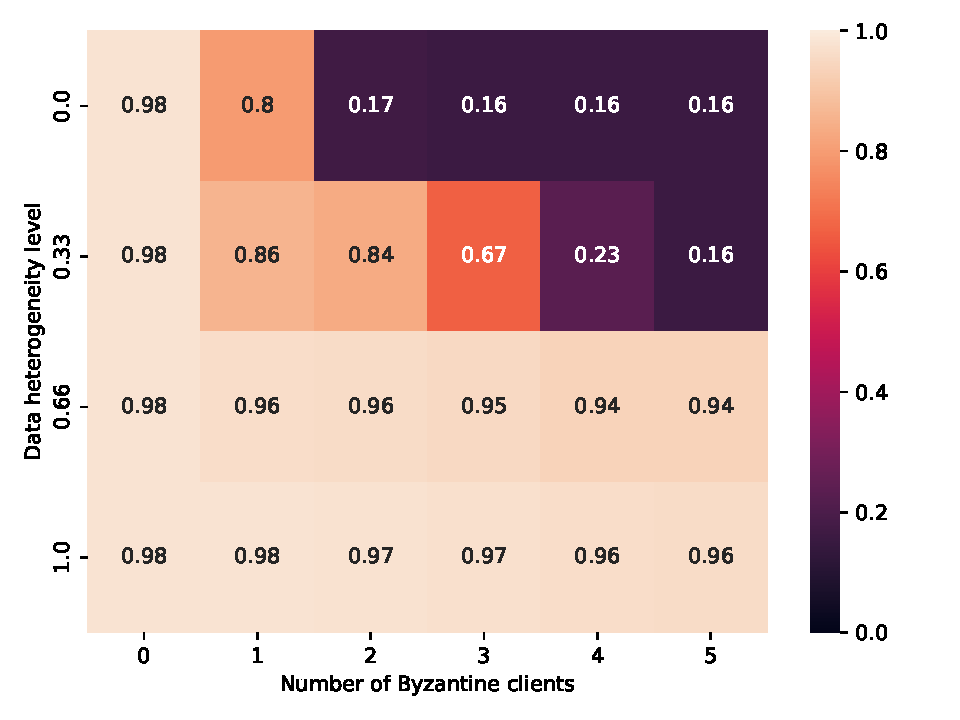
\includegraphics[width=\textwidth]{../plots/mnist_clipping_heatmaps/cnn_mnist_clipping_2/test_mnist_cnn_mnist_clipping_2_gamma_similarity_niid_NNM_ARC_TrMean_nb_honest_clients_10_tolerated_f_equal_real.pdf}
        \caption{CNN ReLU (Clip $=2$)}
        \label{fig:tm_worst_case_clip2}
    \end{subfigure}
    \vspace{0.3cm}
    \begin{subfigure}[b]{0.24\textwidth}
        \centering
        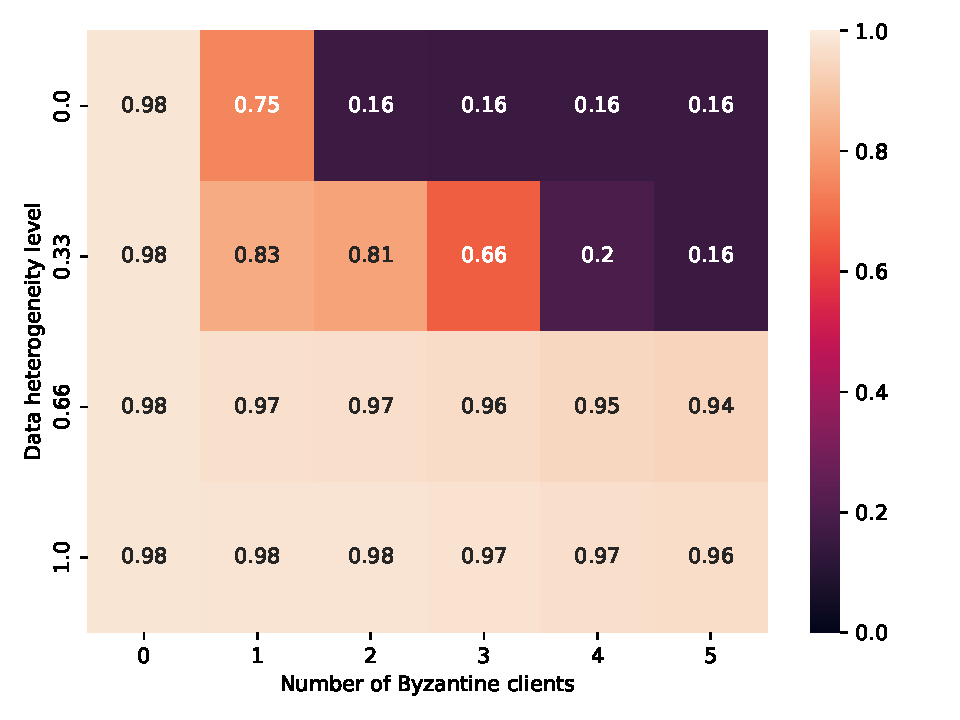
\includegraphics[width=\textwidth]{../plots/mnist_clipping_heatmaps/cnn_mnist_clipping_4/test_mnist_cnn_mnist_clipping_4_gamma_similarity_niid_NNM_ARC_TrMean_nb_honest_clients_10_tolerated_f_equal_real.pdf}
        \caption{CNN ReLU (Clip $=4$)}
        \label{fig:tm_worst_case_clip4}
    \end{subfigure}
    \hfill
    \begin{subfigure}[b]{0.24\textwidth}
        \centering
        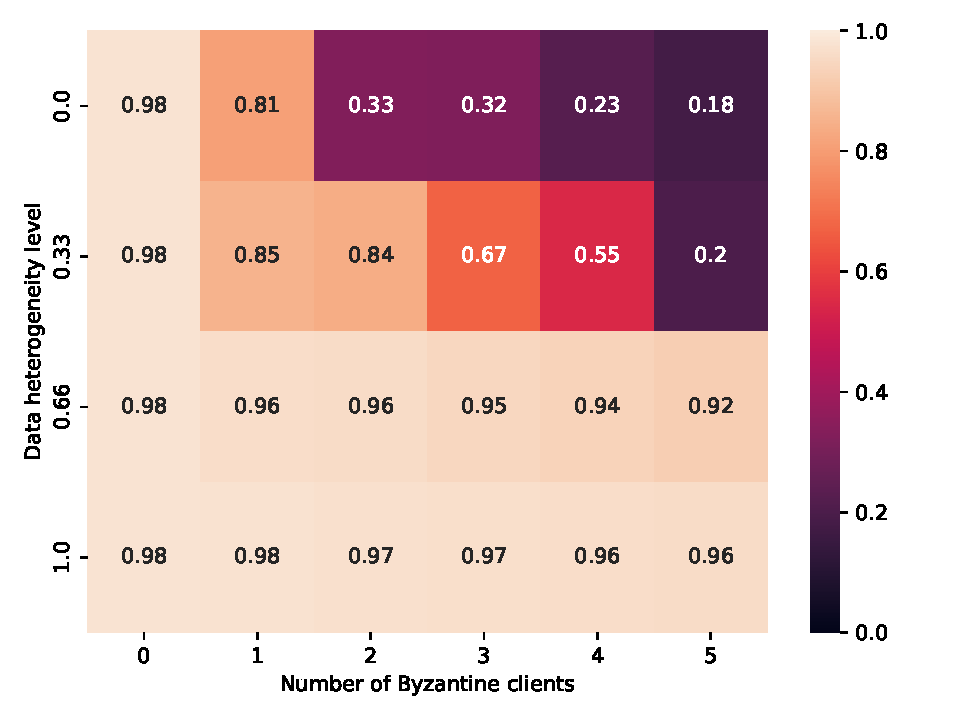
\includegraphics[width=\textwidth]{../plots/cnn_tanh_heatmaps/test_mnist_cnn_mnist_tanh_gamma_similarity_niid_NNM_ARC_TrMean_nb_honest_clients_10_tolerated_f_equal_real.pdf}
        \caption{CNN Tanh}
        \label{fig:tm_worst_case_tanh}
    \end{subfigure}
    \caption{Trimmed Mean (TM) under Worst-Case across all Attacks.}
    \label{fig:tm_worst_case_grid}
\end{figure}
\clearpage
\subsubsection{TM under ALIE}
\begin{figure}[htbp]
    \centering
    \begin{subfigure}[b]{0.24\textwidth}
        \centering
        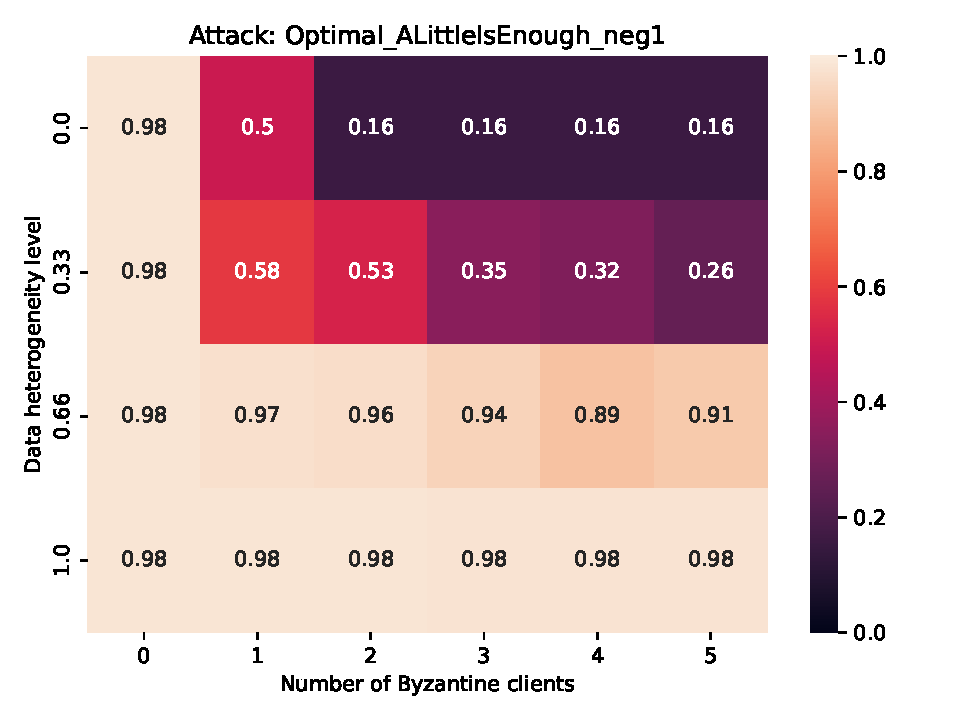
\includegraphics[width=\textwidth]{../plots/mnist_clipping_heatmaps/cnn_mnist/test_Optimal_ALittleIsEnough_neg1_mnist_cnn_mnist_gamma_similarity_niid_NNM_ARC_TrMean_nb_honest_clients_10_tolerated_f_equal_real.pdf}
        \caption{CNN ReLU (No Clip)}
        \label{fig:tm_alie_noclip}
    \end{subfigure}
    \hfill
    \begin{subfigure}[b]{0.24\textwidth}
        \centering
        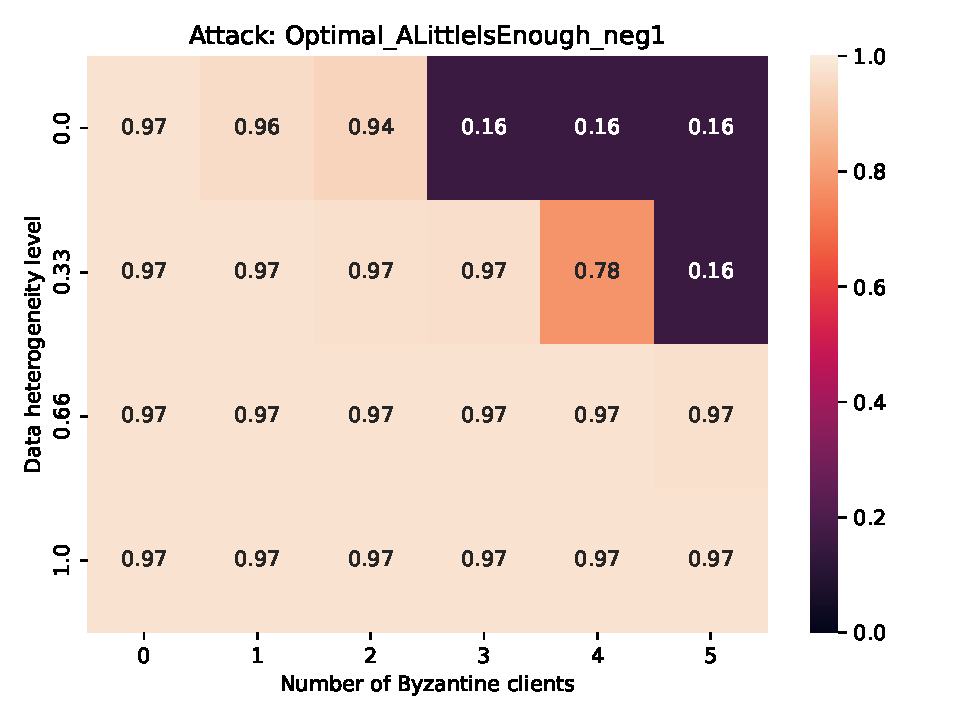
\includegraphics[width=\textwidth]{../plots/mnist_clipping_heatmaps/cnn_mnist_clipping_1/test_Optimal_ALittleIsEnough_neg1_mnist_cnn_mnist_clipping_1_gamma_similarity_niid_NNM_ARC_TrMean_nb_honest_clients_10_tolerated_f_equal_real.pdf}
        \caption{CNN ReLU (Clip $=1$)}
        \label{fig:tm_alie_clip1}
    \end{subfigure}
    \hfill
    \begin{subfigure}[b]{0.24\textwidth}
        \centering
        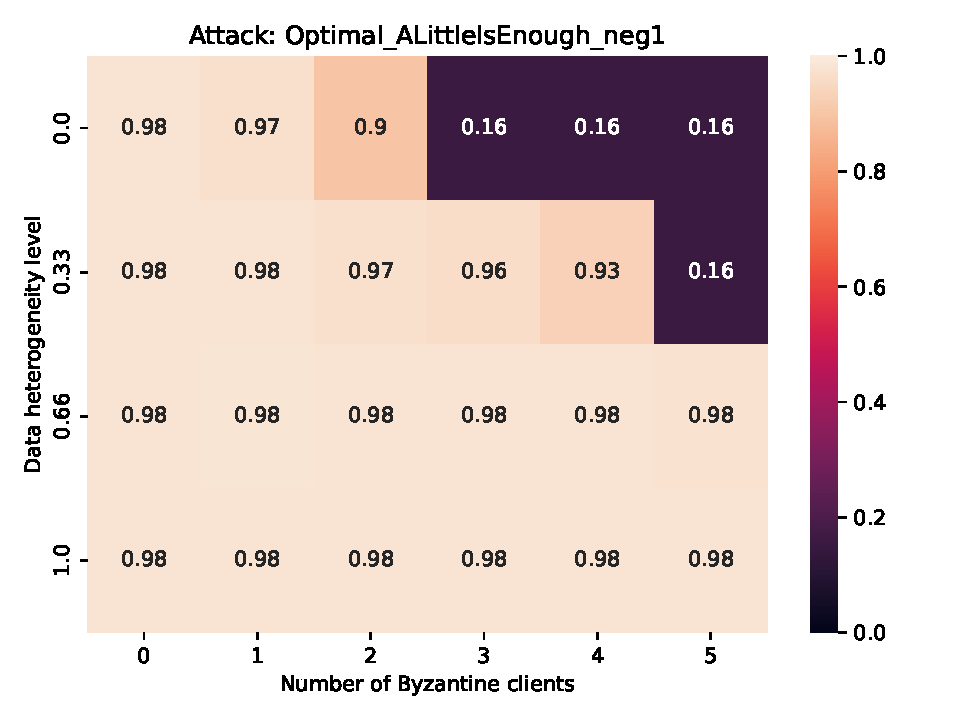
\includegraphics[width=\textwidth]{../plots/mnist_clipping_heatmaps/cnn_mnist_clipping_2/test_Optimal_ALittleIsEnough_neg1_mnist_cnn_mnist_clipping_2_gamma_similarity_niid_NNM_ARC_TrMean_nb_honest_clients_10_tolerated_f_equal_real.pdf}
        \caption{CNN ReLU (Clip $=2$)}
        \label{fig:tm_alie_clip2}
    \end{subfigure}
    \vspace{0.3cm}
    \begin{subfigure}[b]{0.24\textwidth}
        \centering
        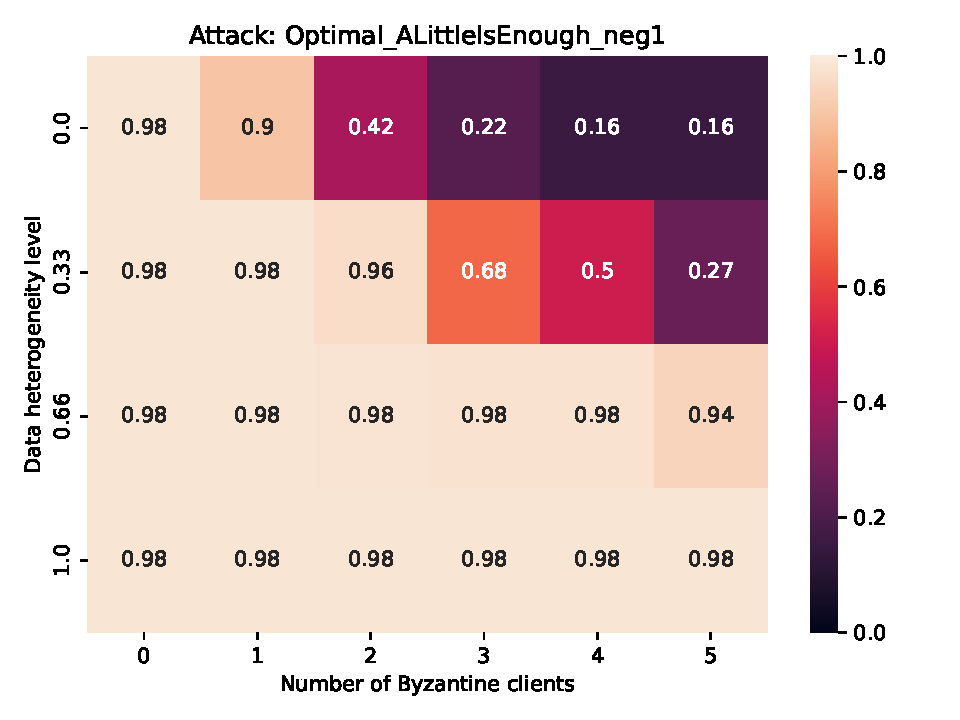
\includegraphics[width=\textwidth]{../plots/mnist_clipping_heatmaps/cnn_mnist_clipping_4/test_Optimal_ALittleIsEnough_neg1_mnist_cnn_mnist_clipping_4_gamma_similarity_niid_NNM_ARC_TrMean_nb_honest_clients_10_tolerated_f_equal_real.pdf}
        \caption{CNN ReLU (Clip $=4$)}
        \label{fig:tm_alie_clip4}
    \end{subfigure}
    \hfill
    \begin{subfigure}[b]{0.24\textwidth}
        \centering
        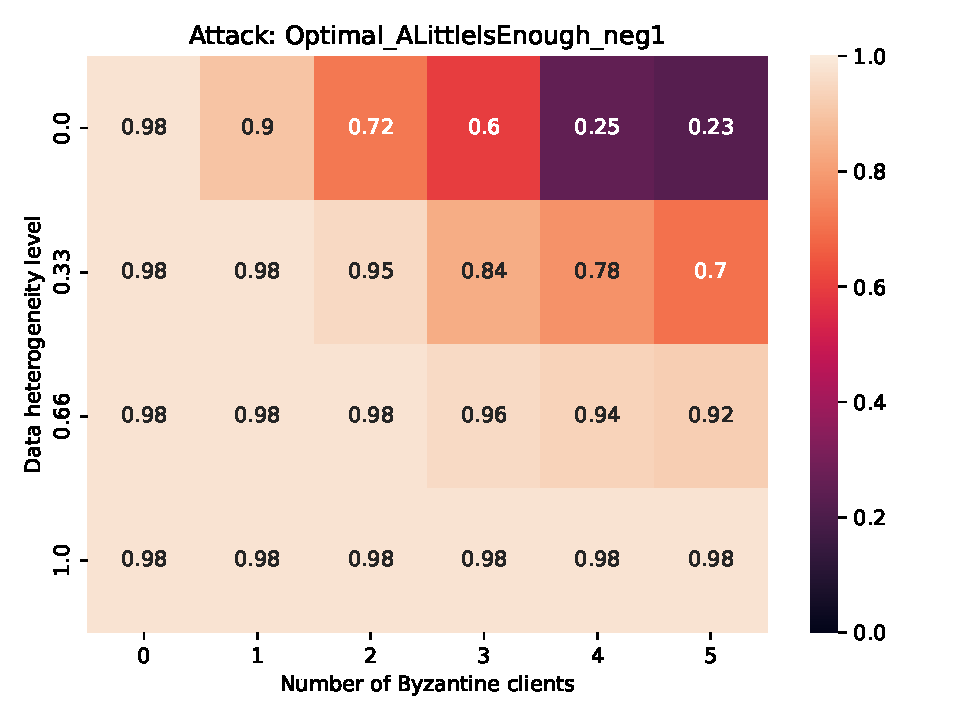
\includegraphics[width=\textwidth]{../plots/cnn_tanh_heatmaps/test_Optimal_ALittleIsEnough_neg1_mnist_cnn_mnist_tanh_gamma_similarity_niid_NNM_ARC_TrMean_nb_honest_clients_10_tolerated_f_equal_real.pdf}
        \caption{CNN Tanh}
        \label{fig:tm_alie_tanh}
    \end{subfigure}
    \caption{Trimmed Mean (TM) under Optimal ALIE Attack.}
    \label{fig:tm_alie_grid}
\end{figure}
\clearpage
\subsubsection{TM under SF}
\begin{figure}[htbp]
    \centering
    \begin{subfigure}[b]{0.24\textwidth}
        \centering
        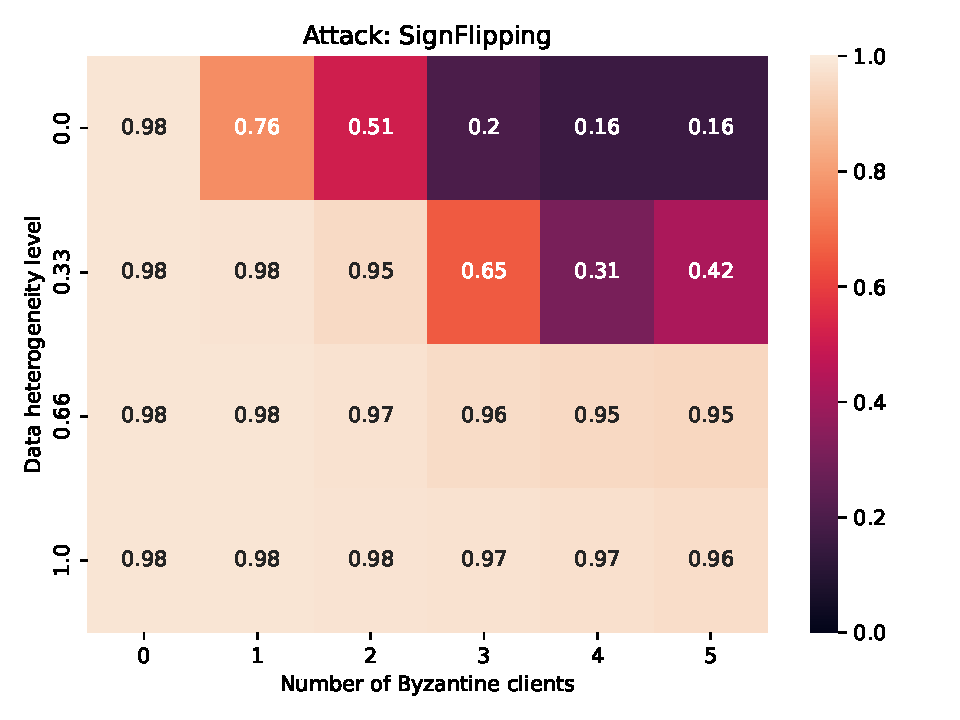
\includegraphics[width=\textwidth]{../plots/mnist_clipping_heatmaps/cnn_mnist/test_SignFlipping_mnist_cnn_mnist_gamma_similarity_niid_NNM_ARC_TrMean_nb_honest_clients_10_tolerated_f_equal_real.pdf}
        \caption{CNN ReLU (No Clip)}
        \label{fig:tm_sf_noclip}
    \end{subfigure}
    \hfill
    \begin{subfigure}[b]{0.24\textwidth}
        \centering
        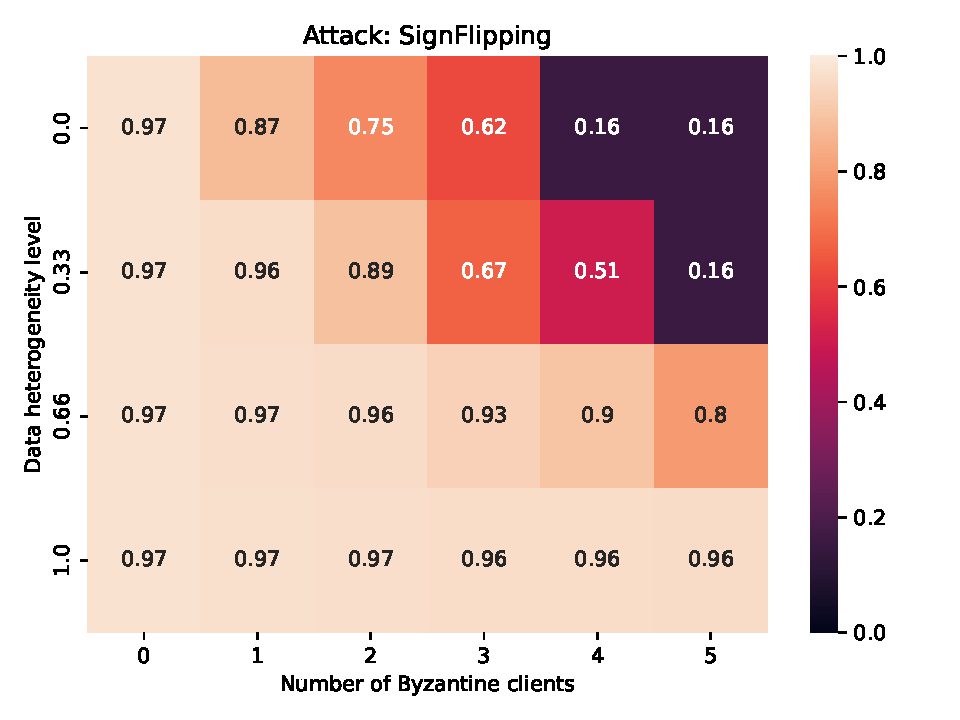
\includegraphics[width=\textwidth]{../plots/mnist_clipping_heatmaps/cnn_mnist_clipping_1/test_SignFlipping_mnist_cnn_mnist_clipping_1_gamma_similarity_niid_NNM_ARC_TrMean_nb_honest_clients_10_tolerated_f_equal_real.pdf}
        \caption{CNN ReLU (Clip $=1$)}
        \label{fig:tm_sf_clip1}
    \end{subfigure}
    \hfill
    \begin{subfigure}[b]{0.24\textwidth}
        \centering
        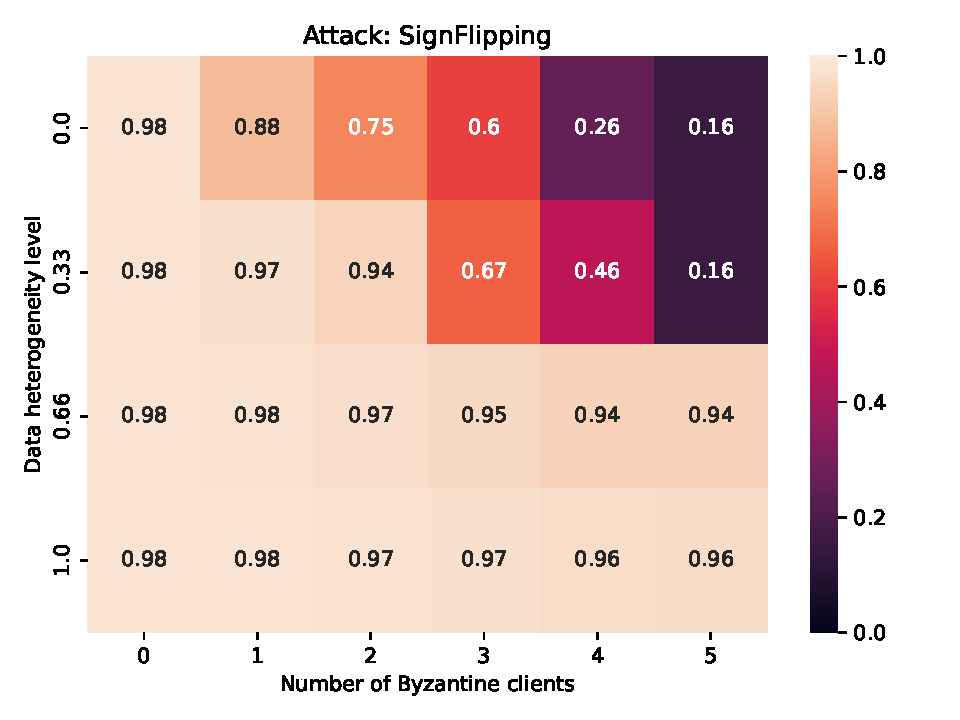
\includegraphics[width=\textwidth]{../plots/mnist_clipping_heatmaps/cnn_mnist_clipping_2/test_SignFlipping_mnist_cnn_mnist_clipping_2_gamma_similarity_niid_NNM_ARC_TrMean_nb_honest_clients_10_tolerated_f_equal_real.pdf}
        \caption{CNN ReLU (Clip $=2$)}
        \label{fig:tm_sf_clip2}
    \end{subfigure}
    \vspace{0.3cm}
    \begin{subfigure}[b]{0.24\textwidth}
        \centering
        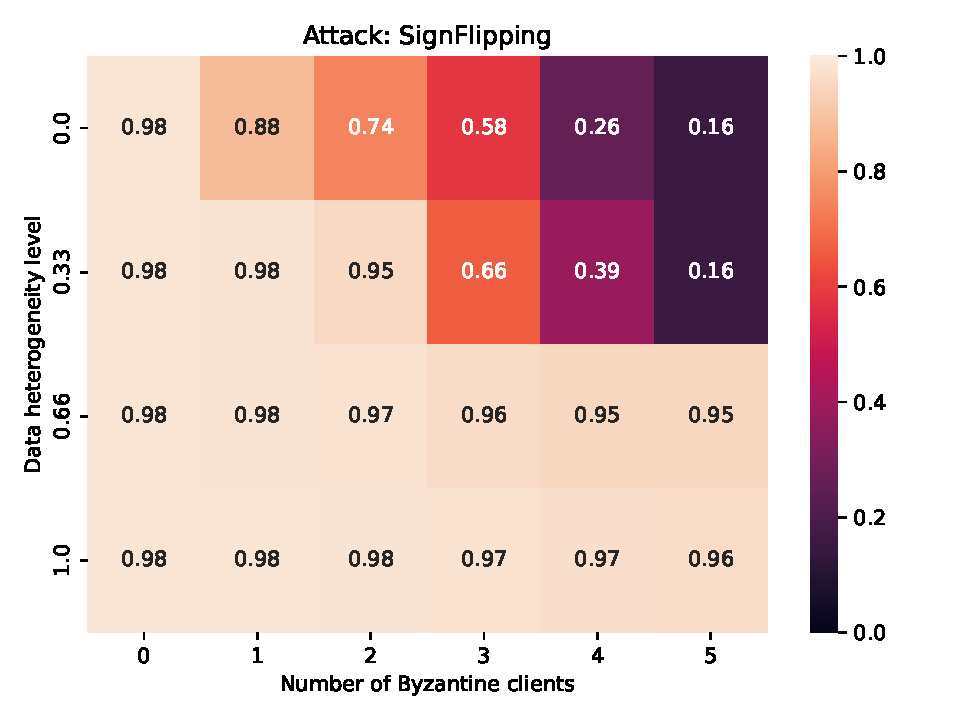
\includegraphics[width=\textwidth]{../plots/mnist_clipping_heatmaps/cnn_mnist_clipping_4/test_SignFlipping_mnist_cnn_mnist_clipping_4_gamma_similarity_niid_NNM_ARC_TrMean_nb_honest_clients_10_tolerated_f_equal_real.pdf}
        \caption{CNN ReLU (Clip $=4$)}
        \label{fig:tm_sf_clip4}
    \end{subfigure}
    \hfill
    \begin{subfigure}[b]{0.24\textwidth}
        \centering
        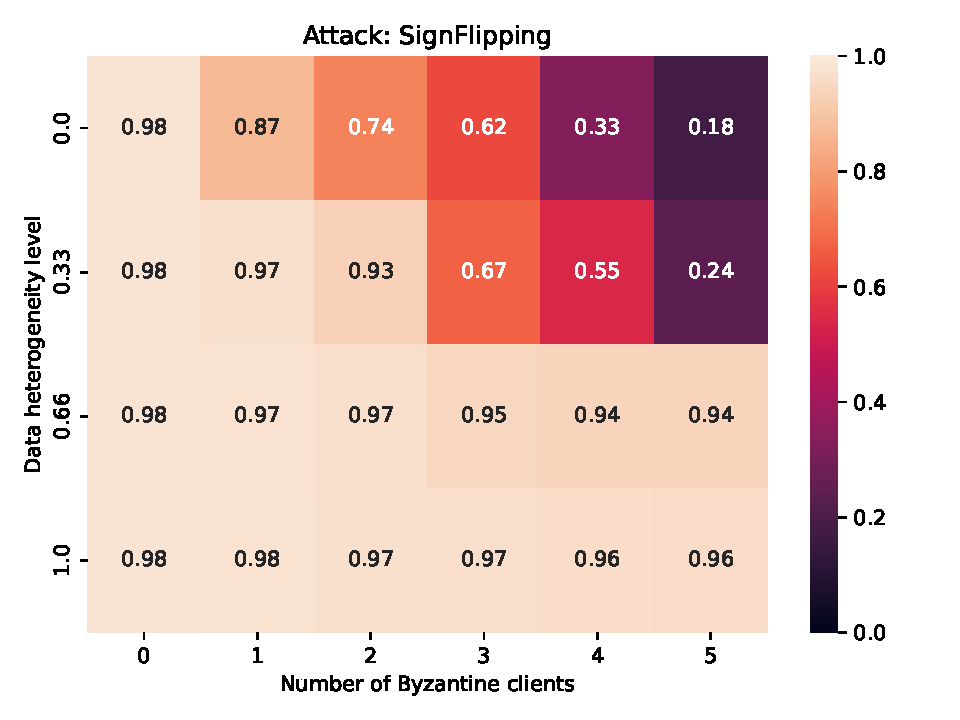
\includegraphics[width=\textwidth]{../plots/cnn_tanh_heatmaps/test_SignFlipping_mnist_cnn_mnist_tanh_gamma_similarity_niid_NNM_ARC_TrMean_nb_honest_clients_10_tolerated_f_equal_real.pdf}
        \caption{CNN Tanh}
        \label{fig:tm_sf_tanh}
    \end{subfigure}
    \caption{Trimmed Mean (TM) under Sign Flipping Attack.}
    \label{fig:tm_sf_grid}
\end{figure}
\clearpage
\subsubsection{TM under IPM}
\begin{figure}[htbp]
    \centering
    \begin{subfigure}[b]{0.24\textwidth}
        \centering
        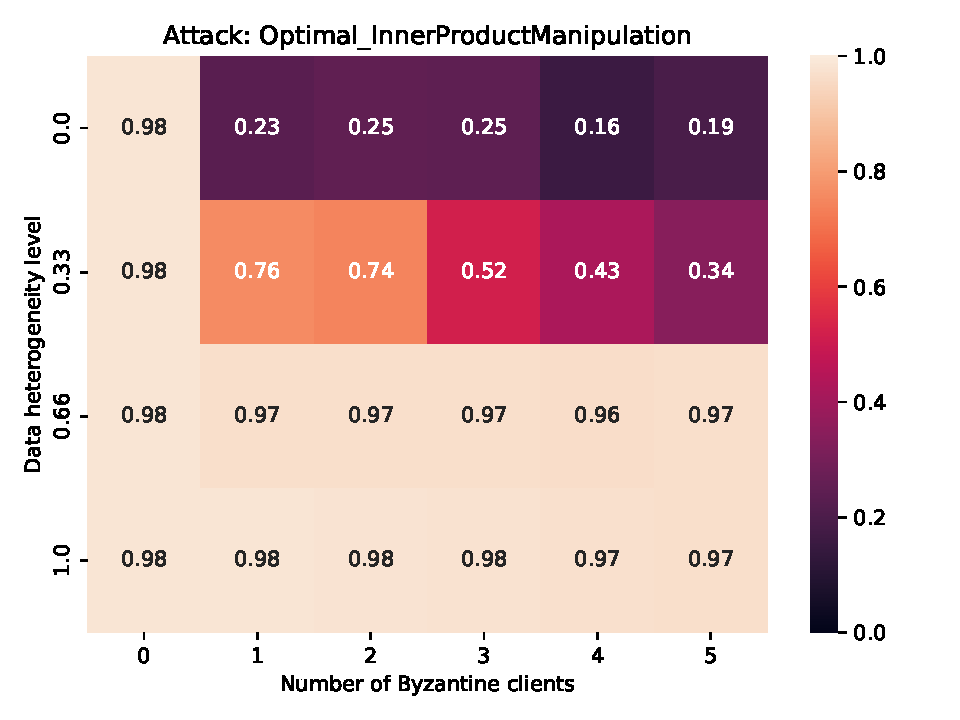
\includegraphics[width=\textwidth]{../plots/mnist_clipping_heatmaps/cnn_mnist/test_Optimal_InnerProductManipulation_mnist_cnn_mnist_gamma_similarity_niid_NNM_ARC_TrMean_nb_honest_clients_10_tolerated_f_equal_real.pdf}
        \caption{CNN ReLU (No Clip)}
        \label{fig:tm_ipm_noclip}
    \end{subfigure}
    \hfill
    \begin{subfigure}[b]{0.24\textwidth}
        \centering
        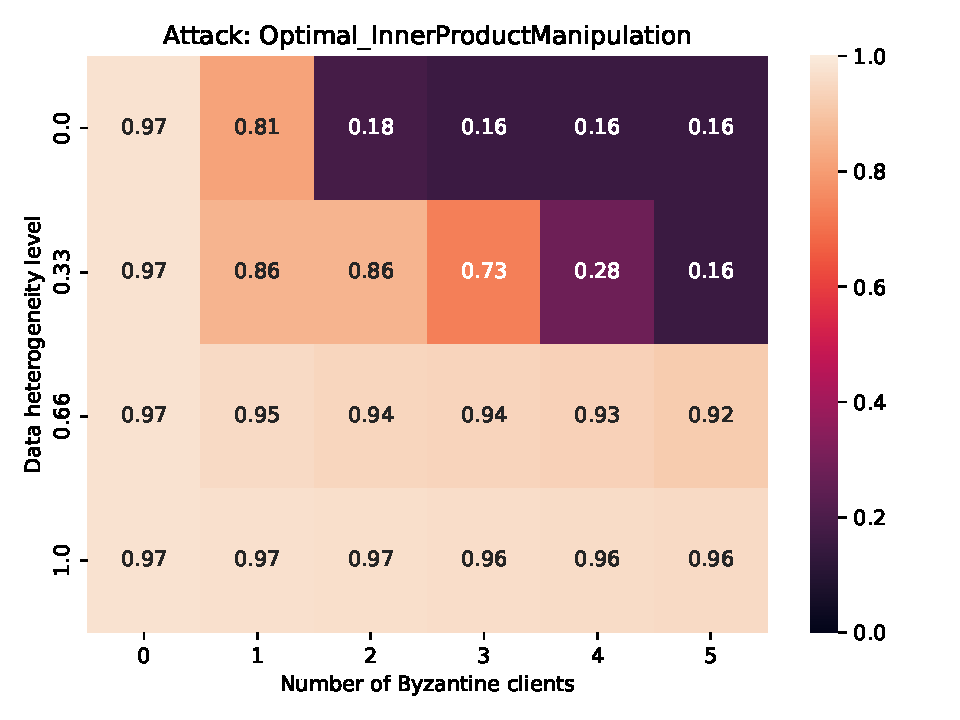
\includegraphics[width=\textwidth]{../plots/mnist_clipping_heatmaps/cnn_mnist_clipping_1/test_Optimal_InnerProductManipulation_mnist_cnn_mnist_clipping_1_gamma_similarity_niid_NNM_ARC_TrMean_nb_honest_clients_10_tolerated_f_equal_real.pdf}
        \caption{CNN ReLU (Clip $=1$)}
        \label{fig:tm_ipm_clip1}
    \end{subfigure}
    \hfill
    \begin{subfigure}[b]{0.24\textwidth}
        \centering
        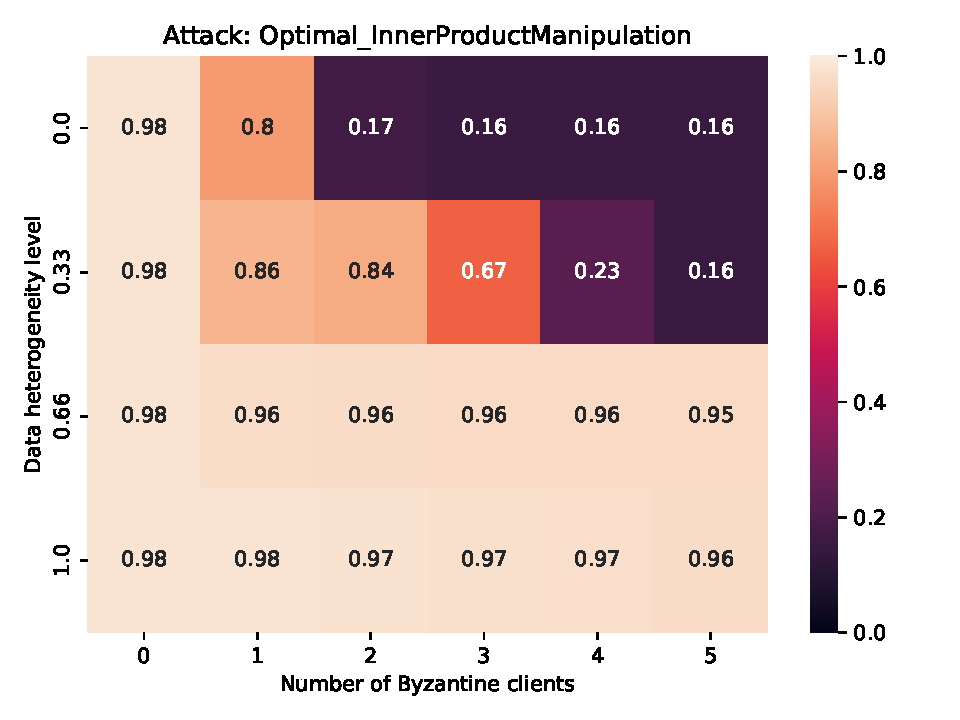
\includegraphics[width=\textwidth]{../plots/mnist_clipping_heatmaps/cnn_mnist_clipping_2/test_Optimal_InnerProductManipulation_mnist_cnn_mnist_clipping_2_gamma_similarity_niid_NNM_ARC_TrMean_nb_honest_clients_10_tolerated_f_equal_real.pdf}
        \caption{CNN ReLU (Clip $=2$)}
        \label{fig:tm_ipm_clip2}
    \end{subfigure}
    \vspace{0.3cm}
    \begin{subfigure}[b]{0.24\textwidth}
        \centering
        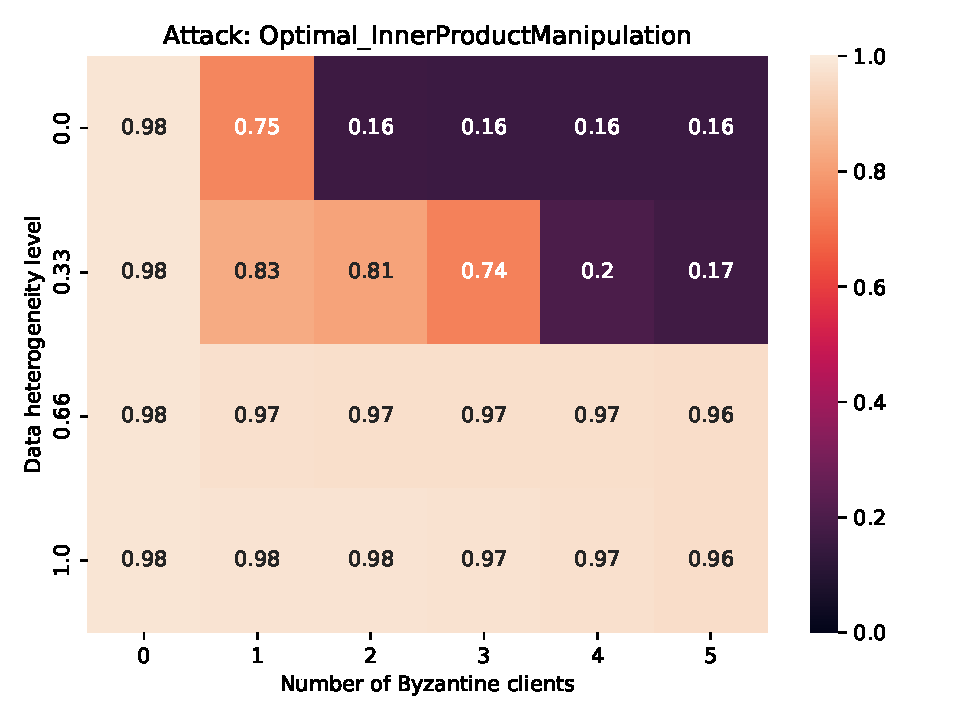
\includegraphics[width=\textwidth]{../plots/mnist_clipping_heatmaps/cnn_mnist_clipping_4/test_Optimal_InnerProductManipulation_mnist_cnn_mnist_clipping_4_gamma_similarity_niid_NNM_ARC_TrMean_nb_honest_clients_10_tolerated_f_equal_real.pdf}
        \caption{CNN ReLU (Clip $=4$)}
        \label{fig:tm_ipm_clip4}
    \end{subfigure}
    \hfill
    \begin{subfigure}[b]{0.24\textwidth}
        \centering
        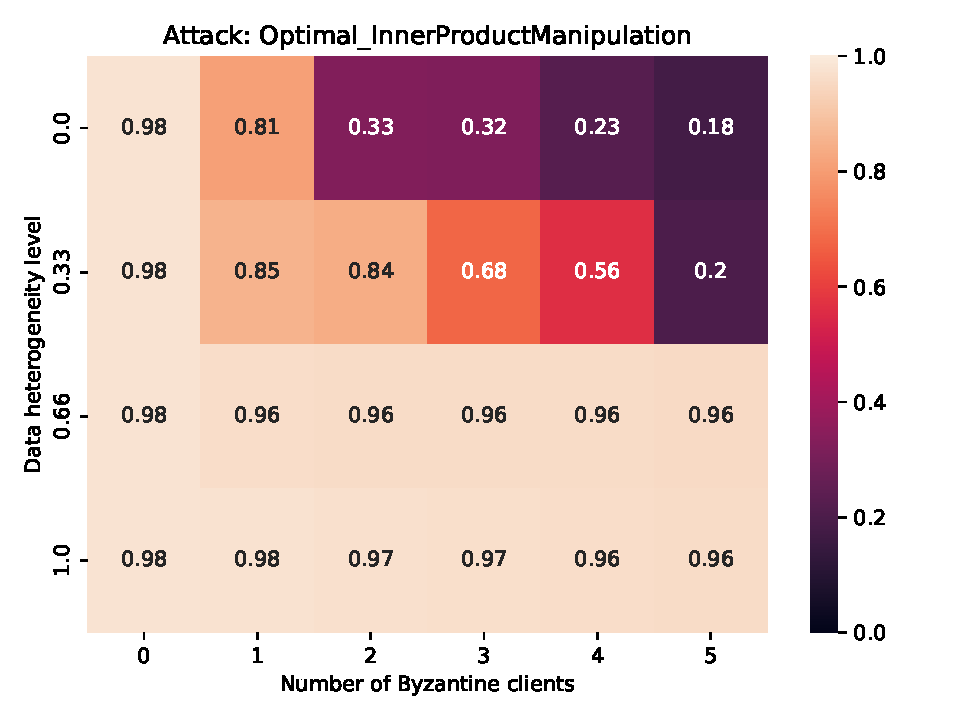
\includegraphics[width=\textwidth]{../plots/cnn_tanh_heatmaps/test_Optimal_InnerProductManipulation_mnist_cnn_mnist_tanh_gamma_similarity_niid_NNM_ARC_TrMean_nb_honest_clients_10_tolerated_f_equal_real.pdf}
        \caption{CNN Tanh}
        \label{fig:tm_ipm_tanh}
    \end{subfigure}
    \caption{Trimmed Mean (TM) under Optimal IPM Attack.}
    \label{fig:tm_ipm_grid}
\end{figure}
\clearpage

\end{document}
